% ==============================================================================
%  $RCSfile: handbuch.tex,v $, $Revision: 1.5 $
%  $Date: 2003/07/06 13:49:09 $
%  $Author: birdy $
%
%  Description: Master Datei des Handbuchs
%
%  Last-Ispelled-Revision:
%
% ==============================================================================

\documentclass[a4paper,titlepage,11pt,german,twoside]{scrbook}


\makeatletter

%koma uses \chapter*, but we want to use \chapter
%  changed srcbook.cls-commands
\renewcommand\idx@heading{%
  \twocolumn
  \chapter{\indexname}\@mkboth{\indexname}{\indexname}
}

%Nummerierung soll net so eng aneinanderhaengen
\renewcommand*\l@section{\@dottedtocline{1}{1.5em}{3em}}

\makeatother


\usepackage{../styles/common}

\usepackage{handbuch}

\usepackage{makeidx}
\makeindex

% subsubsections nummerieren
\setcounter{secnumdepth}{3}

\newcommand\version{Version 1.0\xspace}
%\newcommand\version{\today\xspace}

%\graphicspath{{gui-pictures/}} %OK: it MAY work with graphics. With graphicx, it surely doesn't

% header
\fancyhead{}
\fancyhead[LE,RO]{\slshape \company}
\fancyhead[LO,RE]{\slshape \leftmark}
\fancyfoot[LE,RO]{\thepage{}}
\fancyfoot[LO,RE]{\version}

\begin{document}

% title page
\thispagestyle{empty}
\hfill
\parbox{5.5cm}
{Universit�t Stuttgart\\
Studienprojekt A -- IML Browser\\
\company}

\vspace{3cm}

\begin{center}
  \Huge
  \textsf{Handbuch}\\
  \vspace{.5cm}
  {\Large\version}\\
  \vspace{3cm}
  
\includegraphics[scale=.78]{../logo}
\end{center}
\newpage

%**\section*{Versionsgeschichte}

\begin{itemize}

\item Version 1.0 (08.04.2003)

  Diese Version wurde dem Kunden zur Pr�fung 
  im Kundenreview (14.04.2003 - 16.04.2003) vorgelegt.


\item Version 1.1 (22.04.2003)

  Die Korrekturen gem�� dem Kundenreview vom 14.04.2003 bis
  zum 16.04.2003 wurden eingearbeitet.\\
  Die Spezifikation der GSL (in Version 1.0 noch GQSL) wurde in 
  ein separates Dokument ausgelagert (siehe Kapitel 
  \ref {GIANT Scripting Language}).\\
  Diese Version der Spezifikation ging am 22.04.2003 
  zur Abnahme an den Kunden.

\end{itemize}

%%% Local Variables: 
%%% TeX-master: "spec"
%%% End: 


%===============================================================================
%
% ToDo - Aus fertigem Dokument entferenen
%
% \chapter*{ToDo -- nicht in fertiger Spez.}

% Hier Sachen beschreiben, die irgendwie beim Erstellen der Spez.\ 
% beachtet werden sollen.

% % ==============================================================================
%  $RCSfile: todo_spec.tex,v $ 
%  $Date: 2003/02/04 16:59:34 $
%  $Author: schwiemn $ 
%
%  Description: ToDo File f�r die Spezifikation
%
% ==============================================================================

%===============================================================================
%
% Anforderungen des Kunden
%
\section {Anforderungen des Kunden}
Anbei die Anforderungen des Kunden gem�� der Email vom 30.01.2003

\begin{itemize}

\item Form: DIN A4, gen�gend Platz f�r Korrektur und handschriftliche 
Anmerkungen


\item Gedruckte Dokumentation + PDF

\item Versionierung: Jedes Dokument erh�lt eine Revisionsnummer, 
Erstellungsdatum wird vermerkt

\item Inhaltliche Form: Jedes Dokument verf�gt �ber ein Inhaltsverzeichnis,
Index ist erw�nscht, Seitenzahlen


\item Referenzen: Konsistente globale Nummerierung f�r alle Dokumente
(lebenslang und f�r immer und ewig)

\item Querverweise (nat�rlich innerhalb des selben Dokuments), 
Referenzen auf weitere Dokumente �ber Seite + Abschnitt

\item Inhalt: Begriffslexikon, Konzepte der GUI, 
Erkl�rungen der GUI zum Beispiel anhand abstrakter Bilder,
Usecases mit Zielsetzung spezifizieren

\item vollst�ndige Abdeckung der Anforderungen an das Produkt

\item pr�zise, knapp

\item Traceability: \\
Spezifikation ist der erste Schritt auf dem langen
(und beschwerlichen) Weg zum fertigen Software-Produkt und
dient als Grundlage f�r das weitere Vorgehen.\\
Entwurf, Implementierung und Test referenzieren sie.
Testf�lle f�r den Systemtest sollen aus der Spezifikation
ableitbar sein.


\item Sprache:\\
Wenn Deutsch als Sprache gew�hlt wird, sollten englische Fach-Begriffe
verwendet werden. (Die selben Begriffe werden in Spezifikation
und Implementierung verwendet.)\\
Keine Eindeutschung.\\
Einheitliche Rechtschreibung.

\end{itemize}


%=============================================================================
%
% Mit Kunden zu kl�ren
%
\section {Mit Kunden zu kl�rende Punkte}
Alles was noch offen ist.

\begin{itemize}

\item Interaktionssprache von GIANT (insbeondere der GUI und gegebenfalls innerhalb der Konfigurationsdateien) mit Kunden kl�ren (Deutsch oder Englisch).


\end{itemize}

%===============================================================================
%
% Inhaltsverzeichnis
%
\setcounter{tocdepth}{1}
\tableofcontents

%===============================================================================
%
% Einleitung
%
\chapter{Einleitung}
% ==============================================================================
%  $RCSfile: intro.tex,v $, $Revision: 1.2 $
%  $Date: 2003/07/06 13:39:08 $
%  $Author: birdy $
%
%  Description:
%
%  Last-Ispelled-Revision:
%
% ==============================================================================


\section{�ber dieses Dokument}

Dieses Handbuch beschreibt die Installation und Benutzung des graphischen
IML-Browsers GIANT (Graphical IML Analysis Navigation Tool).

\section{�ber GIANT -- Graphical IML Analysis Navigation Tool}
\index{GIANT}
\index{IML-Browser}

GIANT ist ein Werkzeug, welches an der Universit�t Stuttgart von der 
CodeFabrik@Stuttgart im Rahmen des Studienprojektes A IML-Browser 
des Studiengangs Softwaretechnik entwickelt wurde.\\
Ziel dieser Entwicklung war es, die bereits bestehende HTML-basierte L�sung 
der Bauhaus Reengineering GmbH \index{Bauhaus-Reengineering GmbH}
f�r IML-Graphen durch ein komfortables graphisches Werkzeug zu erg�nzen. 
GIANT erm�glicht es dem Kunden, Teile von gro�en IML-Graphen zu
visualisieren. 
Durch die Unterscheidung der verschiedenen Kanten- und Knotenklassen werden
dar�ber hinaus auch im IML-Graphen enthaltene Analyseergebnisse �bersichtlich
dargestellt.\\

\section{Aufbau dieses Dokuments}

In den ersten Kapiteln dieses Handbuches wird beschrieben, wie Anwender
mit GIANT anhand einiger Beispiele Analysen durchf�hren k�nnen.
Dies wird anhand einer Art Tutorials beschrieben. Dies erm�glicht
erfahrenen Anwendern einen schnellen Start (\gq{Top-Down}) mit GIANT.

In den sp�teren Kapiteln wird GIANT Fenster f�r Fenster und Men�punkt
f�r Men�punkt genau erkl�rt (\gq{Bottom-Up}). Dies erm�glicht auch das
Nachschlagen von Details zu einzelnen Funktionen.



%===============================================================================
%
% Produkt�bersicht
%
\chapter{Produkt�bersicht}

In diesem Kapitel werden einige grundlegende Konzepte und
M�glichkeiten von GIANT vorgestellt und kurz beschrieben.

% ==============================================================================
%  $RCSfile: product.tex,v $, $Revision: 1.34 $
%  $Date: 2003/03/31 22:02:25 $
%  $Author: squig $
%
%  Description: Beschreibung des Produktes. �bersicht �ber die Funktionen
%               und allgemeine Bedienkonzepte.
%
%  Last-Ispelled-Revision: 1.32
%
% ==============================================================================


% ==============================================================================
\section{GIANT Projekte} \index{Projekte} \index{Persistenz}

Innerhalb eines Projektes fasst GIANT Informationen, 
wie erzeugte Anzeigefenster und
erzeugte IML-Teilgraphen f�r einen vorgegebenen IML-Graphen, zusammen
und speichert diese persistent. Die Zusammenfassung zu Projekten soll der 
�bersicht dienen und den Austausch von Teilergebnissen, 
wie z.B. einzelner Anzeigefenster, erleichtern.\\
F�r weitere Informationen zu Projekten siehe 
Kapitel \ref{GIANT Projektverwaltung}.


% ==============================================================================
\section{IML-Teilgraphen und Selektionen}
Hinsichtlich der logischen Zusammenfassung von Knoten und Kanten unterscheidet
GIANT IML-Teilgraphen und Selektionen.

  \subsection{IML-Teilgraphen} \index{IML-Teilgraphen}
  \index{Graph-Knoten} \index{Graph-Kanten} \index{hervorheben} Ein
  IML-Teilgraph beschreibt eine Knoten- und Kantenmenge aus dem
  IML-Graphen bei der jede Kante einen Start- und einen Zielknoten hat
  -- die sogenannten Graph-Knoten und Graph-Kanten.  Die Graph-Knoten
  und Graph-Kanten von IML-Teilgraphen k�nnen in Anzeigefenstern
  hervorgehoben werden. Desweiteren k�nnen die Graph-Knoten und
  Graph-Kanten von IML-Teilgraphen als Fenster-Knoten und
  Fenster-Kanten in Anzeigefenster eingef�gt und layoutet werden.  Die
  IML-Teilgraphen sind aber v�llig unabh�ngig von den Anzeigefenstern
  und enthalten insbesondere keine Layoutinformationen.

  \subsection{Selektionen} \index{Selektionen}
  Selektionen stellen die lokale Variante von Knoten- und Kantenmengen dar.
  Sie sind immer einem festen Anzeigefenster zugeordnet.
  Selektionen k�nnen beliebige Knoten und Kanten umfassen, ohne dass diese 
  einen Teilgraphen bilden m�ssen.
  Jeder Knoten und jede Kante einer Selektion muss auch im Anzeigefenster
  als Fenster-Knoten oder Fenster-Kante vorhanden sein.

% ==============================================================================
\section{Anzeigefenster} \index{Anzeigefenster}
Anzeigefenster sind die Fenster von GIANT, in denen eine benutzerdefinierte
Auswahl von Knoten und Kanten visualisiert wird. Es kann beliebig viele
Anzeigefenster geben und jedes Anzeigefenster kann beliebig viele Selektionen
haben.

  \subsection{Pins} \index{Anzeigefenster!Pins} \index{Pins}
  Da bei gro�en Graphen selten alle zu einem Anzeigeinhalt 
  geh�renden Fenster-Knoten und Fenster-Kanten gemeinsam auf dem Bildschirm
  sichtbar dargestellt werden k�nnen, kann sich der
  Benutzer zu jedem Anzeigefenster eine Liste von Pins anlegen. In den Pins wird
  jeweils die Position des sichtbaren Anzeigeinhaltes und die Zoomstufe
  \index{Zoomstufe}
  gespeichert, so dass zu beliebigen Zeitpunkten die Position des sichtbaren
  Anzeigeinhalts rekonstruiert werden kann.

  \subsection{Visualisierungsstile} \index{Visualisierungsstile}
  Mittels sogenannter Visualisierungsstile kann der Benutzer die
  Darstellung von Fenster-Kanten und Fenster-Knoten auch w�hrend der
  Laufzeit von GIANT beeinflussen.  Da �ber entsprechende XML-Dateien
  verschiedene Visualisierungsstile definiert werden k�nnen, kann
  GIANT so
  an spezifische Problemstellungen angepasst werden.\\
  Weitere Informationen hierzu sind unter Abschnitt \ref{Config
    Visualisierungsstile} verf�gbar.

\section{Knoten-Annotationen} \index{Knoten-Annotationen}
Jeder Knoten kann mit einer textuellen Annotation versehen werden. Diese
Annotation kann in einem Fenster au�erhalb des Anzeigefensters
zur Anzeige gebracht und bearbeitet werden.\\
F�r weitere Informationen hierzu siehe Abschnitt
\ref{Project Persistenz von Knoten-Annotationen}.


% ==============================================================================
\section{Anfragen} \index{GQSL} \index{Anfragesprache}
Eine vielseitige Anfragesprache -- die GIANT Query and Scripting Language GQSL --
stellt nahezu die gesamte Funktionalit�t von GIANT zur Verf�gung und kann 
insbesondere auch zum Aufruf via Kommandozeile
genutzt werden. Die drei Schritte des anschlie�end beschriebenen 
\gq{Drei-Stufen-Konzeptes} k�nnen �ber diese Anfragesprache auch \gq{auf 
einen Schlag} erledigt werden.\\
Die GQSL ist unter Kapitel \ref {GIANT Query Skripting Language} im
Detail spezifiziert.


% ==============================================================================
\section{Drei-Stufen-Konzept} \index{Drei-Stufen-Konzept}

Die im Folgenden beschriebenen drei Schritte sollen dem Benutzer die M�glichkeit
bieten, von den Knoten und Kanten des IML-Graphen ausgehend geeignete
Teilgraphen in Anzeigefenstern zu visualisieren. Von der
Gestaltung der UseCases her, werden diese drei Schritte sequentiell nacheinander
ausgef�hrt, dies ist aber nicht zwingend n�tig.


\begin {enumerate}
  \item Erzeugen geeigneter IML-Teilgraphen, d.h.\ Auswahl geeigneter Knoten 
        und Kanten aus dem IML-Graphen mittels der Anfragesprache.
  
  \item Einf�gen dieser IML-Teilgraphen in ein Anzeigefenster unter Anwendung
  eines Layoutalgorithmus \index{Layoutalgorithmen}. 
  
  \item Weitere Bearbeitung der Fenster-Knoten und Fenster-Kanten (wie z.B.
  Verschieben, Annotieren und Erzeugen von Selektionen).
  
\end {enumerate}








%===============================================================================
% 
% Technische Produktumgebung
%
\chapter{Technische Produktumgebung}

Hier wird die zum Betrieb von GIANT n�tige Hardware 
und die n�tige Software beschrieben.

% ==============================================================================
%  $RCSfile: technical.tex,v $, $Revision: 1.6 $
%  $Date: 2003/09/23 19:33:38 $
%  $Author: birdy $
%
%  Description: Hier sind die Anforderungen an die Programmumgebung 
%  spezifiziert. Dazu geh�ren die verwendete Hard- und Software, sowie
%  Schnittstellen zu anderen Produkten.
%
%  Last-Ispelled-Revision:
%
% ==============================================================================

\section{Software}

\index{Anforderungen!an die Software}

Zum Betrieb von GIANT wird folgende Hardware und Software ben�tigt:
\begin{itemize}
  \item Sun Solaris, Linux oder Windows Betriebssystem
  \item Emacs oder vi Texteditor f�r die Anzeige vom Sourcecode
  \item GTK 2.0 oder h�her
  \item GTKAda 2.2
\end{itemize}


\section{Hardware}

\index{Anforderungen!an die Hardware}
Das Programm l�uft auf SPARC Workstations und x86 kompatiblen PCs.
Im Folgenden sind die minimalen Hardwareanforderungen zur Arbeit mit kleinen 
und mittleren Projekten beschrieben. 
Bei gro�en Projekten ist ein Speicherausbau
von 2 GB und mehr empfehlenswert.

\subsection{Hardwareanforderungen SPARC}

\begin{itemize}
  \item UltraSPARC-II 300 MHz
  \item 512 MB Hauptspeicher
  \item 8 Bit Grafik mit einer min. Aufl�sung von 1024*786
  \item Maus mit mindestens zwei Tasten
\end{itemize}

\subsection{Hardwareanforderungen x86}
\begin{itemize}
  \item Pentium III 600 MHz
  \item 512 MB Hauptspeicher
  \item 8 Bit Grafik mit einer min. Aufl�sung von 1024*786
  \item Maus mit mindestens zwei Tasten
\end{itemize}

\section{Installation}

Die Giant-Installation unter Linux geht folgenderma�en vonstatten:\\

Zun�chst mu� das Installationsarchiv (welches sich im Userverzeichnis,
z.B. /home/sysop befindet), entpackt werden. Bei der GIANT-Version
1.1 ist das entpackte Distributions-Archiv ca. 450 MB gro�.\\

Entpacken des gzip-Archives:

�cd /home/sysop�\\

�gzip -d giant-1.1.0.tar.gz�\\

Entpacken des darin befindlichen Tar-Archives:

�tar xf giant-1.1.0.tar�\\

Im nun existierenden Verzeichnis giant-1.1.0 kann
GIANT mit ./giant gestartet werden.

\section{Compilieren}

GIANT kann durch Ausf�hren von �make� im Verzeichnis
src compiliert werden.




%===============================================================================
%
% Konzepte und Begriffe
%
\chapter{Konzepte und Begriffe}

Dieses Kapitel beschreibt wichtige Begriffe, die f�r das Arbeiten mit
GIANT und das Verst�ndnis dieser Anleitung wichtig sind.

% ==============================================================================
%  $RCSfile: konzepteundbegriffe.tex,v $, $Revision: 1.4 $
%  $Date: 2003/08/05 16:30:52 $
%  $Author: birdy $
%
%  Description:
%
%  Last-Ispelled-Revision:
%
% ==============================================================================


\section{�ber dieses Kapitel}

Dieses Kapitel f�hrt die f�r das Verst�ndnis dieses Handbuches und die
Benutzung von GIANT wichtigen Begriffe ein.
Eine tabellarische Beschreibung der einzelnen Begriffe findet sich
in der Spezifikation von GIANT, Kapitel Begriffslexikon.

\section{Begriffe}

Eine Anfrage (Query) beschreibt einen Vorgang, bei dem
�ber geeignete Kriterien IML-Knoten und IML-Kanten aus dem IML-Graphen
oder aus IML-Teilgraphen ausgew�hlt werden.
GIANT greift �ber eine Schnittstelle, das Reflection Model von Bauhaus
Reengineering, auf den IML-Graphen zu.\\

Die Visualisierung des Graphen erfolgt in Anzeigefenstern.

Mit GIANT k�nnen Teilmengen des IML-Graphen gebildet werden, diese
hei�en IML-Teilgraphen.

In dieser Anleitung weden f�r Knoten und Kanten des Graphen die Begriffe
Fenster-Knoten und Fenster-Kante verwendet, wenn diese in einem Anzeigefenster
sichtbar sind, oder allgemein IML-Knoten bzw. IML-Kante.
Die Namen Graph-Knoten und Graph-Kante werden verwendet, wenn Knoten bzw.
Kante Bestandteil eines IML-Teilgraphen sind.
    

Der Begriff Kantenklasse (Edge Class) bezeichnet die Einteilung der
IML-Kanten des IML-Graphen in verschiedene Klassen, wie sie sich aus der
IML-Graph-Bibliothek von Bauhaus ergibt.\\

Die Zuordnung einer IML-Kante zu einer Kantenklasse wird durch die Knotenklasse
des Start-Knotens und den Namen des Attributes (aus dem Bauhaus-IML-Graphen),
welches die IML-Kante beschreibt, festgelegt. Jede vorkommende Kombination aus
der Knoten-Klasse eines Start-Knotens und dem Namen eines Attributes,
welches eine Kante beschreibt, ist somit eine eigene Kantenklasse.\\

Eine Knotenklasse (Node Class) ergibt sich aus der Einteilung der IML-Knoten
des IML-Graphen in verschiedene Klassen, wie sie sich aus der
IML-Graph-Bibliothek von Bauhaus ergibt.\\

Eine Klassenmenge (Class Set) ist eine durch die IML-Graph Bibliothek
vorgegebene Zusammenfassung von Kantenklassen und Knotenklassen.
Es kann mehrere Klassenmengen geben. Die selben Knotenklassen und 
Kantenklassen k�nnen gleichzeitig zu mehreren Klassenmengen geh�ren.\\

Eine Knoten-Annotationen (Node Annotation ist eine eine textuelle
Beschreibung zu einem bestimmten Knoten des IML-Graphen, die der Nutzer
hinzuf�gen kann.\\
    
Die zweidimensionale r�umliche Anordnung von
Fenster-Knoten und Fenster-Kanten innerhalb eines Anzeigefensters
auf dem sogenannten Anzeigeinhalt wird Layout genannt.\\
  
Eine Auswahl von Fenster-Knoten und Fenster-Kanten 
eines visualisierten Teilgraphen des IML-Graphen innerhalb eines
Anzeigefensters. hei�t Selektion (Selection).\\
  
Selektieren (to select) beschreibt einen Vorgang �ber den der Benutzer, z.B.
durch Anklicken von Fenster-Knoten oder Fenster-Kanten mit der Maus,
eine Selektion aufbaut.
  


  
Der Nutzer kann in GIANT-Anzeigefenster zoomen, d.h. die Zoomstufe
(Zoom Level) jedes Fensters ver�ndern.  Dieser Faktor beschreibt die Gr��e des
sichtbaren Anzeigeinhaltes.  Bei einer sehr niedrigen Zoomstufe
(auch: weit weg gezoomt) ist ein gr��erer Teil des im
Anzeigefenster visualisierten IML-Graphen sichtbar als bei einer
hohen Zoomstufe (auch: sehr nach heran gezoomt).\\
  
Hervorheben von Knoten bedeutet, dass in einem
Anzeigefenster visualisierte Fenster-Knoten oder Fenster-Kanten
z.B. durch eine farbige Umrahmung von anderen Fenster-Knoten oder
Fenster-Kanten unterscheidbar gemacht werden.\\
    
\section{Bezeichnertypen} \label{afa Bezeichnertypen}
 Hier werden Bezeichnertypen, also von GIANT als f�r z.B. Fensternamen zul�ssig akzeptierte
 Folgen von Ziffern, Buchstaben und Sonderzeichen definiert.

    \begin {enumerate}
  
      \item
      Die lateinischen Gro�- und Kleinbuchstaben; nicht zul�ssig sind
      Umlaute und das Zeichen ''"s''. Zul�ssig sind also nur die 
      ASCII-Zeichen 65 bis 90 und 97 bis 122 (gem�� Spezifikation
      der ISO-8859-Zeichens�tze).
   
      \item
      Die Ziffern ''0'' bis ''9'' (ASCII-Zeichen 48 bis 57)
    
      \item
      Das Zeichen ''\_'' (ASCII-Zeichen 95).
     
    \end {enumerate}

\section {Allgemeine Bedienkonzepte} \index{Bedienkonzepte}
Hier werden grundlegende Konzepte der Bedienung von GIANT beschrieben.

  \subsection {Selektieren von Fenster-Knoten und Fenster-Kanten in 
               Anzeigefenstern}
  \label {Selektieren von Fenster-Knoten und Fenster-Kanten in 
               Anzeigefenstern} 

  \index{Selektieren}
  
  Hier werden die Abl�ufe zur Selektion und Deselektion einzelner
  Fenster-Knoten und Fenster-Kanten mittels der Maus und
  Tastatur aufgez�hlt.\\
  Die so erzielte Auswahl bezieht sich immer auf die aktuelle
  Selektion (siehe Selektionsauswahlliste im Fenster).
    
  Allgemein gilt: Selektiert werden kann mit der Maus durch Klick
  mit der linken Maustaste oder Aufziehen eines Rahmens mittels der
  gedr�ckten linken Maustaste.
    
  Falls w�hrend des Selektierens mit der Maus (beide Methoden) die Shift-Taste
  auf der Tastatur gedr�ckt gehalten wird, so werden die markierten
  Knoten und Kanten der bisherigen Selektion hinzugef�gt, bzw. entfernt, wenn diese
  schon hinzugef�gt waren.
  Wird w�hrend des Aufziehens eines Rahmens mit der linken Maustaste
  die Control-Taste auf der Tastatur niedergedr�ckt gehalten, so
  werden alle Knoten und Kanten innerhalb des Rahmens hinzugef�gt, egal,
  ob diese schon markiert waren.
    
  \begin{enumerate}

   \item Alle selektierten Fenster-Knoten und Fenster-Kanten deselektieren.\\
   Wird mit der linken Maustaste auf einen Punkt des sichtbaren Anzeigeinhaltes
   geklickt, unter dem sich keine Fenster-Knoten bzw. Fenster-Kanten befinden,
   so werden alle bis dahin selektierten Fenster-Knoten und Fenster-Kanten
   deselektiert.
  
   \item Selektieren durch Anklicken mit linker Maustaste.\\
   Nur der angeklickte Fenster-Knoten oder die angeklickte Fenster-Kante 
   wird selektiert. 
   Andere bis dahin selektierte Fenster-Knoten und Fenster-Kanten 
   werden deselektiert.
   
   \item Selektieren durch Anklicken mittels Shift + linke Maustaste.\\
   Falls noch nicht selektiert wird der angeklickte Fenster-Knoten oder die
   angeklickte Fenster-Kante zu der aktuellen Selektion hinzugef�gt.
   Falls bereits selektiert, wird der Fenster-Knoten oder die Fenster-Kante 
   aus der aktuellen Selektion entfernt.
   
   \index{Rahmen}
   \item Selektieren durch Aufziehen eines Rahmens mittels gedr�ckter 
   linker Maustaste.\\
   Alle Fenster-Knoten und Fenster-Kanten innerhalb des Rahmens werden 
   selektiert, alle Fenster-Knoten und Fenster-Kanten au�erhalb des 
   Rahmens werden deselektiert.
   
   \item Selektieren durch Aufziehen eines Rahmens mittels 
   Shift + gedr�ckte linke Maustaste.\\
   Alle Fenster-Knoten und Kanten innerhalb des Rahmens, 
   die noch nicht selektiert sind, werden der aktuellen Selektion 
   hinzugef�gt.\\
   Alle Fenster-Knoten und Kanten innerhalb des Rahmens, 
   die bereits selektiert
   sind, werden aus der aktuellen Selektion entfernt.

   \item Selektieren durch Aufziehen eines Rahmens mittels 
   Control + gedr�ckte linke Maustaste.\\
   Alle Fenster-Knoten und Fenster-Kanten innerhalb des Rahmens, 
   die noch nicht selektiert sind, werden der aktuellen Selektion 
   hinzugef�gt. Fenster-Knoten und Kanten innerhalb und au�erhalb 
   des Rahmens, die bereits selektiert sind, bleiben selektiert.
  
  \end{enumerate}

  Der Nutzer kann z.B. 

  \subsection{Standard-Selektion}
  \label{Standard-Selektion}
  \index{Standard-Selektion}
 
  Jedes Anzeigefenster hat genau eine Standard-Selektion. Diese
  Selektion wird bei der Erzeugung des Fensters angelegt und ist zu
  Anfang leer. Die Standard-Selektion kann nicht gel�scht
  werden. Abgesehen davon verh�lt sich die Standard-Selektion wie vom
  Benutzer angelegte Selektionen.
    
  \subsection {Aktuelle Selektion} 
               \label{Aktuelle Selektion vs Selektionen}

  \index{Aktuelle Selektion}
               
  \begin{enumerate}
  
  \item Es gibt zu jedem Anzeigefenster beliebig viele Selektionen
    (mindestens aber eine -- die Standard-Selektion),
    davon ist immer eine die aktuelle Selektion.
    
    \item 
    Das oben beschriebene Selektieren mittels der linken Maustaste 
    und weiterer Funktionstasten (siehe 
    \ref{Selektieren von Fenster-Knoten und Fenster-Kanten in Anzeigefenstern}) 
    betrifft immer nur die aktuelle Selektion. \\
    Alle anderen Selektionen k�nnen zwar hervorgehoben werden, aber nicht 
    durch das Selektieren mittels linker Maustaste etc. ge�ndert werden.
      
    \item
    Der Benutzer kann jederzeit mittels Kontextmen� bestimmen, welche der
    Selektionen eines Anzeigefensters die aktuelle Selektion ist.
    
    \item 
    Die aktuelle Selektion wird immer hervorgehoben. 
  
  \end {enumerate}
  
  
  
\section {Verhalten beim Einf�gen von IML-Teilgraphen und Selektionen
in Anzeigefenster}
  \label{Verhalten beim Einf�gen von IML-Teilgraphen und Selektionen
         in Anzeigefenster}

  \index{IML-Teilgraphen!Einf�gen in Anzeigefenster}
  \index{Selektionen!Einf�gen in Anzeigefenster}
  
  In diesem Abschnitt wir der Einf�gevorgang von IML-Teilgraphen und
  Selektionen in Anzeigefenster spezifiziert.

   \subsection {Vorgabe der Zielposition} \index{Zielposition}
     \label{Vorgabe der Zielposition}
   F�r bestimmte Funktionen muss der Benutzer manuell Zielpositionen
   innerhalb eines zu bestimmenden Anzeigefensters ausw�hlen. An dieser
   Zielposition werden dann z.B. neue Fenster-Knoten eingef�gt. Ablauf:
   
   \begin {enumerate}
   
     \item
     Der Benutzer w�hlt das entsprechende Anzeigefenster aus
     (dadurch dass er ihm je nach Betriebssystemkonvention den
     Fokus gibt). Hierbei k�nnen nur bereits ge�ffnete Anzeigefenster
     des Projektes ausgew�hlt werden.
     
     \item
     Befindet sich die Maus �ber dem Bereich des Anzeigefensters, wo
     der IML-Graph visualisiert wird, so wird anstatt des
     Mauszeigers ein Fadenkreuz (siehe auch \ref{Fadenkreuzcursor}) angezeigt.
     
     \item
     Durch Klicken mit der linken Maustaste wird dann �ber das Fadenkreuz die
     Zielposition vorgegeben.
     
   \end{enumerate}
   
   
   \subsection {Automatisches Erzeugen neuer Selektionen im Zielfenster}
   S�mtliche Fenster-Knoten und Fenster-Kanten, die in einem Schritt in
   ein Anzeigefenster eingef�gt werden, werden dort automatisch
   zur Standard-Selektion, der alte Inhalt der Standard-Selektion geht 
   dabei verloren und die Standard-Selektion bekommt den Status der 
   aktuellen Selektion.
    
   \subsection{Einf�gen von Selektionen in Anzeigefenster}
      \label{Einf�gen von Selektionen in Anzeigefenster}

   \index{Selektionen!Einf�gen in Anzeigefenster}

   Hier wird das grundlegende Verhalten beim Einf�gen von Selektionen
   in Anzeigefenster (Kopieren einer Selektion aus einem Anzeigefenster
   in ein anderes) beschrieben.
   
   \begin{enumerate}
   
     \item
     Das Layout der Selektion wird beim Einf�gen in ein Anzeigefenster
     �bernommen.
     
     \item
     Die Position von Fenster-Knoten der einzuf�genden Selektion, 
     die bereits in dem Anzeigefenster visualisiert sind,
     bleibt, falls nicht an entsprechender Stelle anders
     spezifiziert, unver�ndert.
     
     \item
     Fenster-Kanten der Selektion werden nur eingef�gt, 
     falls ihr Start- und ihr Zielknoten
     ebenfalls Bestandteil der Selektion sind oder bereits im Anzeigefenster
     visualisiert sind. 
     
     \item
     Die neu eingef�gte Selektion ist in dem entsprechenden 
     Anzeigefenster (dort wo sie eingef�gt wurde) als Standard-Selektion 
     vorhanden, der alte Inhalt der Standard-Selektion wird �berschrieben.
   
   \end{enumerate}
     
  
   \subsection{Einf�gen von IML-Teilgraphen in Anzeigefenster}
     \label{Einf�gen von IML-Teilgraphen in Anzeigefenster}
   \index{IML-Teilgraphen!Einf�gen in Anzeigefenster}

   Hier wird das grundlegende Verhalten des Systems 
   beim Einf�gen von IML-Teilgraphen in Anzeigefenster beschrieben.
   
   \begin{enumerate}
   
     \item
     Das Layout f�r den IML-Teilgraphen wird vor dem Einf�gen gem�� eines
     vom Benutzer vorgegebenen Layoutalgorithmus berechnet.
     
     \item
     Die Graph-Knoten und Graph-Kanten des IML-Teilgraphen werden dann
     analog zu  \ref{Einf�gen von Selektionen in Anzeigefenster} 
     als Fenster-Knoten und Fenster-Kanten in das Anzeigefenster eingef�gt
       
   \end{enumerate} 
  
  
% ==============================================================================  
\section {Verhalten bei Umwandeln von Selektionen und IML-Teilgraphen}
  \label{Verhalten bei Umwandeln von Selektionen und IML-Teilgraphen}

  \index{Umwandeln von Selektionen und IML-Teilgraphen}


  Dieser Abschnitt beschreibt grundlegende Konventionen f�r die
  Umwandlung von IML-Teilgraphen in Selektionen und umgekehrt.


  \subsection {Selektion aus IML-Teilgraphen ableiten}
    \label{Selektion aus IML-Teilgraphen ableiten}

  \index{Selektionen!Ableiten aus IML-Teilgraphen}

  \begin {enumerate}
  
    \item
    Der IML-Teilgraph bleibt unver�ndert.
  
    \item
    Im zu bestimmenden Anzeigefenster wird eine neue Selektion erzeugt,
    die alle Graph-Knoten und Graph-Kanten des IML-Teilgraphen umfasst, 
    welche bereits
    als Fenster-Knoten und Fenster-Kanten im Anzeigefenster vorhanden sind.
    
    \item
    Knoten und Kanten des IML-Teilgraphen, die nicht als Fenster-Knoten und
    Fenster-Kanten im entsprechenden Anzeigefenster vorhanden sind, werden
    ignoriert.
 
  \end {enumerate}
  
    
  \subsection {IML-Teilgraph aus Selektion ableiten}
    \label{IML-Teilgraphen aus Selektion ableiten}

   \index{IML-Teilgraphen!Ableiten aus Selektionen}

  \begin {enumerate}
  
    \item
    Die Selektion bleibt unver�ndert.
    
    \item
    Es wird ein neuer IML-Teilgraph erzeugt. Dieser umfasst alle Knoten 
    und Kanten der Selektion, welche einen g�ltigen Teilgraphen bilden.
    Kanten der Selektion, deren Start- und Zielknoten nicht ebenfalls
    Bestandteil der Selektion sind, werden ignoriert.
 
  \end {enumerate}
  

\section {Verhalten beim Entfernen von Fenster-Knoten und Fenster-Kanten}
  \label{Verhalten beim Entfernen von Fenster-Knoten und Fenster-Kanten}

  \index{Fenster-Knoten!entfernen}
  \index{Fenster-Kanten!entfernen}

  
  Beim Entfernen von Fenster-Knoten und Fenster-Kanten aus einem
  Anzeigefenster werden nur die graphischen Repr�sentationen der IML-Knoten und
  IML-Kanten des Bauhaus-IML-Graphen in dem betroffenen Anzeigefenster 
  gel�scht.
  Graph-Knoten und Graph-Kanten von IML-Teilgraphen bleiben davon unber�hrt.
 
  \subsection {Entfernen aller Knoten und Kanten einer Selektion}
    \label {Entfernen aller Knoten und Kanten einer Selektionen}

    \index{Selektionen!Entfernen von Knoten und Kanten}

  Beim Entfernen aller Fenster-Knoten und Fenster-Kanten einer Selektion
  gelten die folgenden Konventionen:
  
  \begin {enumerate}
  
    \item
    Alle Fenster-Knoten und Fenster-Kanten der Selektion werden aus dem
    Anzeigefenster entfernt.
    
    \item
    Fenster-Kanten im Anzeigefenster, deren Start- oder Zielknoten
    entfernt wird, werden ebenfalls entfernt (auch wenn sie nicht
    zur entsprechenden Selektion geh�ren).
            
    \item 
    Andere Selektionen des Anzeigefensters werden entsprechend aktualisiert, 
    die betroffenen Fenster-Knoten und Fenster-Kanten werden auch aus 
    diesen Selektionen entfernt.

  \end{enumerate}



\section {Auseinanderschieben von Fenster-Knoten}
  \label {Auseinanderschieben von Fenster-Knoten}

  \index{Fenster-Knoten!auseinanderschieben}
  \index{auseinanderschieben}
  
Sollen Fenster-Knoten auf dem Anzeigeinhalt automatisch
auseinandergeschoben werden, so geschieht dies nach dem hier beschriebenen
Modus.
GIANT stellt diese Funktionalit�t dem Benutzer �ber einen
UseCase zur manuellen Ausf�hrung zur Verf�gung. Ein automatisches 
\gq{Auseinanderschieben von Fenster-Knoten} durch GIANT selbst ist
nicht vorgesehen, der Entwurf wird aber eine einfache Erweiterbarkeit
von GIANT diesbez�glich unterst�tzen.

\begin {enumerate}

  \item
  Es gibt einen fixen Punkt, von dem aus alle Fenster-Knoten weggeschoben
  werden.
  
  \item 
  Die Fenster-Knoten werden immer entlang einer Strecke von diesem 
  Punkt durch den jeweiligen Fenster-Knoten verschoben.
  
  \item
  Jeder Fenster-Knoten wird um einen konstanten Betrag (kann vom Benutzer 
  eingegeben werden) von dem Punkt weggeschoben.
 
\end {enumerate}


%===============================================================================
% 
% Tutorial
%
\chapter{Tutorial}
\label{Tutorial}

Dieses Kapitel beschreibt einige h�ufig vorkommende Analysen mit GIANT
und wie sie vom Benutzer ausgef�hrt werden k�nnen.

%**% =============================================================================
%  $RCSfile: fa.tex,v $, $Revision: 1.7 $
%  $Date: 2003/02/19 10:55:17 $
%  $Author: schwiemn $
%
%  Description:
%
% =============================================================================

\section{Der Aktor \gq{Benutzer}}
Aktor im Sinne der anschlie�end spezifizierten UseCases ist immmer die 
menschliche Person, die den IML-Browser GIANT gerade benutzt, also der 
\gq{Benutzer}. Da GIANT keinen Mehrbenutzerbetrieb vorsieht, ist dies immer 
eine einzige Person. 
Neben dem \gq{Benutzer} sind keine weiteren Aktoren vorgesehen.\\


  \subsection{Anforderungen an den Aktor \gq{Benutzer}}
  GIANT ist eine Profi-Werkzeug. Weder das System noch das Handbuch richten 
  sich an unerfahrene Benutzer. Zur Bedienung muss der Benutzer daher 
  zwingend �ber die folgenden Kenntnisse verf�gen:

  \begin{itemize}
    \item Erfahrung im Umgang mit grafischen GUIs und 
          dem entsprechenden Betriebssystem.
  
    \item Grundkenntnisse in XML 
          (nur f�r das Editieren der Konfigurationsdateien).

    \item Erfahrung im Bereich Reengineering.

    \item Kenntnisse �ber Struktur und Aufbau des IML-Graphen. 

  \end{itemize}


% =============================================================================
\section{Starten von GIANT}

Der Benutzer startet das Programm GIANT durch ausf�hren der entsprechenden
Programmdatei. Hierbei hat er bez�glich eventueller Kommandozeilenparameter
die folgenden Optionen. 

  \subsubsection {M�gliche Parameter}
  \begin {enumerate}
    
    \item loadiml=''Pfad''\\
    Angabe des Pfades zu einer existierenden IML-Graph Datei.
      
    \item loadproject=''Pfad''\\
    Angabe des Pfades zu einer existierenden Projektdatei.
      
    \item executequery=''Anfrage''\\
    Eingabe eines Wortes der Anfragespreche als String.
     
    \item loadquery=''Pfad''\\
    Pfad zu einer Datei in der ein Wort der Anfragespreche gespeichert ist.
      
  \end {enumerate}
      
  \subsection {M�gliche Aufrufe}

  \begin {enumerate}
  
    \item Eingabe von: <giant>\\
    GIANT startet und ziegt das Main Window an. 
    Es ist noch kein Projekt geladen.
    
    \item Eingabe von: <giant -loadiml=''my\_iml\_file''>\\
    Neues Projekt (erh�lt einen Default-Namen) wird ge�ffnet.
    Dieses Projekt ist noch nicht persistent gespeichert.
    \label{Kommandozeile_neus}

    \item Eingabe von: <giant -loadproject=''my\_project\_file''>\\
    Das angegebene Projekt wird ge�ffnet.
    \label{Kommandozeile_altes}
    
    \item
    Bei \ref{Kommandozeile_neus} und \ref{Kommandozeile_altes}
    kann zus�tzlich entweder der Parameter\\
    <... -executequery''my\_query\_string''> oder der Parameter\\
    <... -loadquery''my\_query\_file''> eingegeben werden.\\
    In diesem Falle wird dann die �bergebene Anfrage ausgef�hrt.
    Die Ergebnisse werden dem neuen oder dem bestehenden Projekt 
    hinzugef�gt, sind aber noch nicht persistent gespeichert.


  \end {enumerate}
  
% ==============================================================================
\section{Beenden von GIANT}
Giant kann durch Schlie�en des HAUPTFENSTERS oder durch Auswahl 
des entsprechenden Eintages im Hauptmen� oder durch ALT+F4 beendet werden.\\
Ablauf:

\begin {enumerate}
  \item Der Benutzer gibt das Kommando zum Beenden von GIANT.
  \item GIANT fragt nach, ob das Projekt gespeichert werden soll.
  (PROJEKT SPEICHERN) (ENTSPRCHENDER DIALOG MUSS IN DIE GUI)
\end {enumerate}
  



% =============================================================================
% Use Cases
  
% ==============================================================================
%  $RCSfile: load_store.tex,v $, $Revision: 1.24 $
%  $Date: 2003/04/19 17:40:56 $
%  $Author: birdy $
%
%  Description: UseCases f�r Lade- und Speicherfunktionalit�t
%
%  Last-Ispelled-Revision: 1.12
%
% ==============================================================================

\begin{uc}[Neues Projekt]{UC: Neues Projekt}
\index{Projekte!neues Projekt erstellen}
  Erstellt ein neues GIANT Projekt. Ein eventuell bereits ge�ffnetes
  Projekt wird dabei geschlossen, wobei �nderungen auf Nachfrage 
  vorher gespeichert werden.
  Weitere wichtige Informationen, die in engem Zusammenhang mit 
  diesem UseCase stehen, sind unter dem Abschnitt 
  \ref{Project Persistenz der Projekte} zu finden.\\
  Zul�ssige Namen f�r Projekte sind unter Abschnitt 
  \ref{afa Zulaessige Namen} spezifiziert.
  
  
  \begin{precond}
    \cond Das Programm ist gestartet.
  \end{precond}

  \begin{postsuccess}
    \cond Ein neues GIANT Projekt mit dem eingegebenen Namen 
          ist erstellt und geladen.   

    \cond Eine IML-Datei ist geladen.

    \cond Das angegebene Projektverzeichnis ist gegebenenfalls 
          (falls es noch nicht vorhanden war) erstellt 
          worden (siehe \ref {Project Das Projektverzeichnis}).

    \cond Die neu erstellte Projektdatei 
          (siehe \ref{Project Die Projektdatei})
          liegt im Projektverzeichnis.
 
    \cond Ein eventuell zuvor ge�ffnetes Projekt ist geschlossen.
          �nderungen an dem eventuell zuvor ge�ffneten Projekt sind je
          nach Entscheidung des Benutzers bei der entsprechenden 
          Sicherheitsabfrage gespeichert oder verworfen.

  \end{postsuccess}

  \begin{postfail}
    \cond Das System bleibt im bisherigen Zustand, falls der
          Benutzer den UseCase mit Cancel abgebrochen hat.

    \cond Tritt w�hrend des Erstellens des neuen Projektes,
          nachdem das eventuell zuvor ge�ffnete Projekt
          geschlossen wurde, ein Fehler auf, so bleibt das Verhalten
          des Systems unspezifiziert.

  \end{postfail}
  
  \begin{proc}
    \step[1]
    Der Benutzer startet den UseCase �ber das Men� Project
    (siehe \ref{Main-Window-Project}) durch Auswahl von \gq{New Project}.

    \step[2]
    GIANT zeigt den Standard-Filechooser-Dialog und fordert den
    Benutzer auf eine vorhandene IML-Graph Datei auszuw�hlen.
  
    \step[3] Der Benutzer w�hlt im Standard-Filechooser-Dialog
    eine IML-Datei aus und best�tigt
    seine Eingabe mit OK (siehe \ref{Standard-Filechooser-Dialog}).
    
    \step[4]
    GIANT zeigt erneut den Standard-Filechooser-Dialog und fordert den
    Benutzer zur Eingabe des Namens der Projektdatei auf.

    \step[5] Der Benutzer gibt im Standard-Filechooser-Dialog
    den Pfad und den Namen der Projektdatei (\gq{Please select Project
    Path and Project File Name}) ein, die Dateiendung wird sp�ter
    von GIANT automatisch gesetzt. Der Name der Projektdatei ist
    automatisch auch der Name f�r das Projekt. Das Verzeichnis der
    Projektdatei wird automatisch zum Projektverzeichnis.

    \step[6]
    Der Benutzer best�tigt er seine Eingabe mit OK.\\
    Existiert die eingegebene Projektdatei bereits, 
    erscheint eine Fehlermeldung gem�� den unter Abschnitt 
    \ref{afa Fehlerverhalten} beschriebenen Konventionen.\\
    Existiert in dem Projektverzeichnis bereits eine andere Projektdatei, so 
    erscheint ebenfalls eine Fehlermeldung.\\
    
    \step[7] Falls noch ein Projekt ge�ffnet ist, erscheint eine 
    Sicherheitsabfrage (siehe \ref{Sicherheitsabfrage})
    ob dieses gespeichert werden soll.    
    Entscheidet der Benutzer sich f�r Speichern, so wird
    die unter \ref{Alles Speichern} beschriebene Funktionalit�t 
    ausgef�hrt. Lehnt der Benutzer dies ab, gehen
    alle nicht gespeicherten Informationen verloren.\\
     
    \step[8]
    GIANT schlie�t das aktuell ge�ffnete Projekt (falls eines ge�ffnet war), 
    legt, falls noch nicht vorhanden, ein neues Projektverzeichnis an,
    erzeugt ein neues Projekt und �ffnet dieses.
       
  \end{proc}

  \begin{aproc}
    \astep{3} Der Benutzer bricht die Verarbeitung mit Cancel ab.  
    \astep{5} Der Benutzer bricht die Verarbeitung mit Cancel ab.
  \end{aproc}
\end{uc}

% ==============================================================================

\begin{uc}[Projekt �ffnen]{UC: Projekt �ffnen}
\index{Projekte!�ffnen}
  �ffnet ein GIANT Projekt. Ein eventuell bereits ge�ffnetes
  Projekt wird dabei geschlossen, wobei �nderungen auf Nachfrage 
  vorher gespeichert werden. \\ 
  Sollte der Benutzer die XML-Dateien 
  innerhalb des Projektverzeichnisses (siehe 
  \ref{Project Das Projektverzeichnis}) manuell modifiziert haben, so
  dass diese von den durch GIANT automatisch erstellten Dateien
  abweichen, wird keinerlei Garantie f�r das korrekte �ffnen
  des Projektes �bernommen. Das Verhalten
  bez�glich eventuell auftretender Fehler ist undefiniert.

  \begin{precond}
    \cond Das Programm ist gestartet.
  \end{precond}

  \begin{postsuccess}
    \cond Das gew�nschte GIANT Projekt ist geladen.
    \cond Die zugeh�rige IML-Datei ist geladen.
    \cond �nderungen an einem eventuell zuvor ge�ffneten Projekt sind 
          je nach Wahl des Benutzers bei der Sicherheitsabfrage gespeichert
          oder verworfen.

  \end{postsuccess}

  \begin{postfail}
    \cond Hat der Benutzer den UseCase mit Cancel abgebrochen, 
          bleibt das System im bisherigen Zustand.

    \cond Muss der UseCase w�hrend des Ladens des neuen Projektes
          aufgrund eines Fehlers abgebrochen werden, so 
          kehrt das System falls m�glich in einen Zustand zur�ck,
          der dem Start des Systems ohne �ffnen eines Projektes
          entspricht.

    
  \end{postfail}
  
  \begin{proc}    
    \step[1]
    Der Benutzer startet den UseCase �ber das Men� Project
    (siehe \ref{Main-Window-Project} Men�) durch Auswahl von \gq{Load Project}.
    GIANT zeigt daraufhin den Standard-Filechooser-Dialog und fordert
    den Benutzer zur Auswahl eines zu �ffnenden Projektes auf.
    
    \step[2] 
    Der Benutzer w�hlt aus dem Standard-Filechooser-Dialog (siehe 
    \ref {Standard-Filechooser-Dialog})
    eine vorhandene GIANT Projektdatei (siehe \ref{Project Die Projektdatei}) 
    aus und best�tigt mit OK.
    
    \step[3] Falls bereits ein Projekt ge�ffnet ist, erscheint eine 
    Sicherheitsabfrage (siehe \ref{Sicherheitsabfrage})
    ob dieses gespeichert werden soll.     
    Entscheidet der Benutzer sich f�r Speichern, so wird
    die unter \ref{Alles Speichern} beschriebene Funktionalit�t 
    ausgef�hrt. Lehnt der Benutzer dies ab, gehen
    alle nicht gespeicherten Informationen verloren.\\

    
    \step[4]
    GIANT schlie�t das alte Projekt (falls eines ge�ffnet war)
    und l�dt das angegebene neue Projekt.

  \end{proc}

  \begin{aproc}
    \astep{2} Der Benutzer bricht die Verarbeitung mit Cancel ab.
  \end{aproc}
\end{uc}

% ==============================================================================

\begin{uc}[Projekt speichern]{UC: Projekt speichern}  
\index{Projekte!speichern}
  Speichert alle �nderungen an einem Projekt. Der Zustand der
  entsprechenden Verwaltungsdateien im Projektverzeichnis entspricht
  nach erfolgreicher Ausf�hrung dieses UseCases exakt dem aktuellen
  Zustand des ge�ffneten Projektes. Alle Konventionen zur
  Persistenz von Projekten sind im Abschnitt 
  \ref{Project Persistenz der Projekte} exakt spezifiziert.

  \begin{precond}
    \cond Das Programm ist gestartet.

    \cond Ein Projekt ist ge�ffnet. 

  \end{precond}

  \begin{postsuccess}
    \cond Die Informationen des Projekts 
    (einschlie�lich aller m�glichen �nderungen) sind persistent in die
    Verwaltungsdateien geschrieben.
 
  \end{postsuccess}

  \begin{postfail}
    \cond Das System bleibt im bisherigen Zustand.
  \end{postfail}
   
  \begin{proc}    
    \step[1]
    Der Benutzer startet den UseCase �ber das Men� Project
    (siehe \ref{Main-Window-Project}) durch Auswahl von \gq{Save Project}.
      
    \step[2]
    GIANT f�hrt die unter \ref{Alles Speichern} beschriebene Funktionalit�t 
    aus und speichert alle Informationen zu dem Projekt in der zugeh�rigen
    Projektdatei.
  \end{proc}

\end{uc}



% ==============================================================================

\begin{uc}[Projekt speichern unter]{UC: Projekt speichern unter}
\index{Projekte!unter neuem Namen speichern}
Speichert alle Informationen zu einem Projekt in eine neue Projektdatei
(entsprechende Verwaltungsdateien werden ebenfalls dupliziert).


  \begin{precond}
    \cond Das Programm ist gestartet.
    \cond Ein Projekt ist ge�ffnet (entweder ein neu erzeugtes oder ein
          geladenes).
  \end{precond}

  \begin{postsuccess}
    \cond Eine neue Projektdatei ist erzeugt worden.

    \cond Das angegebene Projektverzeichnis ist, falls es noch
          nicht vorhanden war, erstellt worden.

    \cond Die Daten des Projekts sind persistent in die 
          neuen Verwaltungsdateien im Projektverzeichnis 
          der neuen Projektdatei geschrieben (siehe auch
          \ref{Project Persistenz der Projekte}).
        
    \cond Das aktuell ge�ffnete Projekt bleibt in GIANT ge�ffnet, 
          zuk�nftiges Speichern
          (siehe \ref{Projekt speichern}) betrifft nur die 
          Verwaltungsdateien im neu erzeugten Projekt.

    \cond Die alte Projektdatei und alle zugeh�rigen Verwaltungsdateien 
          bleiben unver�ndert.
    
 
  \end{postsuccess}

  \begin{postfail}
    \cond Das System bleibt im bisherigen Zustand.
  \end{postfail}
  
  \begin{proc}    
    \step[1]
    Der Benutzer startet den UseCase �ber das Men� Project
    (siehe \ref{Main-Window-Project}) durch Auswahl von \gq{Save Project As...}.
    Daraufhin zeigt GIANT den Standard-Filechooser-Dialog und fordert
    den Benutzer auf den Namen und den Ort (Pfad) der neuen Projektdatei
    einzugeben.

     
    \step[2] Der Benutzer gibt im Standard-Filechooser-Dialog 
             (siehe \ref {Standard-Filechooser-Dialog}) 
             das neue Projektverzeichnis 
             (siehe \ref{Project Das Projektverzeichnis})
             und den Namen f�r die neue Projektdatei
             (siehe \ref{Project Die Projektdatei}) ein, die Dateiendung 
             wird sp�ter von GIANT automatisch gesetzt. \\
    Der Name der Projektdatei ist automatisch auch der Name f�r das Projekt.
    Zul�ssige Namen sind unter Abschnitt \ref{afa Zulaessige Namen}
    spezifiziert. \\ Das Verzeichnis, welches f�r die Projektdatei 
    angebenen wurde, wird automatisch zum Projektverzeichnis. 
  
    \step[3]  
    Der Benutzer best�tigt seine Eingabe mit OK.\\
    Existiert die eingegebene Datei schon, erscheint eine Fehlermeldung.\\
    Existiert in dem angegebenen Projektverzeichnis 
    bereits eine andere Projektdatei, so erscheint eine entsprechende 
    Fehlermeldung.\\

    \step[4]
    GIANT speichert das alte Projekt in der neuen Projektdatei,
    falls noch nicht vorhanden wird auch das neue Projektverzeichnis
    angelegt. Alle Verwaltungsdateien werden ebenfalls im neuen
    Projektverzeichnis gespeichert.
  
  \end{proc}


 \begin{aproc}
    \astep{2} Der Benutzer bricht die Verarbeitung mit Cancel ab.  
 \end{aproc}
\end{uc}







% ==============================================================================
%  $RCSfile: gui_window.tex,v $, $Revision: 1.34 $
%  $Date: 2003/04/05 21:08:37 $
%  $Author: squig $
%
%  Description: UseCases f�r die Fensterfunktionalit�t der GUI
%
%  Last-Ispelled-Revision: 1.25
%
% ==============================================================================

\begin{uc}[Leeres Anzeigefenster erzeugen]{UC: Leeres Anzeigefenster erzeugen}
\index{Anzeigefenster!erzeugen}

�ber diesen UseCase kann der Benutzer neue Anzeigefenster innerhalb eines
Projektes anlegen.

  \begin{precond}
    \cond Ein Projekt ist geladen.
  \end{precond}

  \begin{postsuccess}
    \cond Das neue, leere Anzeigefenster ist ge�ffnet.
    \cond Das neue Anzeigefenster ist Bestandteil des Projektes.
  \end{postsuccess}

  \begin{postfail}
    \cond Das System bleibt im bisherigen Zustand.
  \end{postfail}
  
  \begin{proc}    
    \step[1] 
    Der Benutzer startet den UseCase �ber das Popup Men�
    \ref{WINDOW-LIST-POPUP} durch Auswahl von \gq{New Window}.        
    
    \step[2]
    GIANT erzeugt ein neues Anzeigefenster (siehe  \ref{GUI Anzeigefenster})
    mit einem Namen nach dem Schema ,,Unknown\_??'' und �ffnet dies.
  \end{proc}

  \begin{aproc}
    \ageneral Es sind keine alternativen Abl�ufe vorgesehen.
  \end{aproc}
\end{uc}


% ==============================================================================
\begin{uc}[Anzeigefenster �ffnen]{UC: Anzeigefenster �ffnen}
\index{Anzeigefenster!�ffnen}

Dient zum �ffnen eines Anzeigefensters des Projektes.

  \begin{precond}
    \cond Ein Projekt mit mindestens einem Anzeigefenster ist geladen.
    \cond Es gibt mindestens ein nicht ge�ffnetes Anzeigefenster.
  \end{precond}

  \begin{postsuccess}
    \cond Das Anzeigefenster ist ge�ffnet.
  \end{postsuccess}

  \begin{proc}    
    \step[1]
    Der Benutzer f�hrt einen Doppelklick auf ein nicht ge�ffnetes
    Anzeigefenster in der Liste �ber die Anzeigefenster
    (siehe \ref{WINDOW-LIST}) durch, oder w�hlt im zugeh�hrigen Popup Men�
    \ref{WINDOW-LIST-POPUP} den Eintrag ,,Open'' aus.
   
    \step[2]
    GIANT �ffnet das entsprechende Anzeigefenster.
  \end{proc}  

\end{uc}

% ==============================================================================
\begin{uc}[Anzeigefenster umbenennen]{UC: Anzeigefenster umbenennen}
\index{Anzeigefenster!umbenennen}

Dient zum Umbenennen eines Anzeigefensters des Projektes.

  \begin{precond}
    \cond Ein Projekt mit mindestens einem Anzeigefenster ist geladen.
  \end{precond}

  \begin{postsuccess}
    \cond Das Anzeigefenster hat einen neuen Namen.
  \end{postsuccess}

  \begin{postfail}
    \cond Es sind keine Fehlerf�lle vorgesehen.
  \end{postfail}

  \begin{proc}    
    \step[1]
    Der Benutzer f�hrt einen Rechtsklick auf ein Anzeigefenster in der Liste
    �ber die Anzeigefenster (siehe \ref{WINDOW-LIST}) durch und w�hlt im
    Popup Men� \ref{WINDOW-LIST-POPUP} den Eintrag ,,Rename'' aus.

    \step[2] 
    GIANT �ffnet den allgemeinen Texteingabedialog 
    \gq{Enter Name For Window} (siehe \ref{DIALOG-WINDOW}).

    \step[3]
    Der Benutzer gibt dort einen zul�ssigen Namen f�r das Anzeigefenster ein
    und best�tigt seine Eingabe mit OK.
    
    \step[4]
    GIANT benennt das Anzeigefenster (siehe \ref{GUI Anzeigefenster}) um.
  \end{proc}  

  \begin{aproc}
    \ageneral Es sind keine alternativen Abl�ufe vorgesehen.
  \end{aproc}
\end{uc}


% ==============================================================================
\begin{uc}[Anzeigefenster speichern]{UC: Anzeigefenster speichern}
\index{Anzeigefenster!speichern}

Mit diesem UseCase wird ein Anzeigefenster gespeichert.
N�heres zur Persistenz von Anzeigefenstern ist unter Abschnitt
\ref{Project Persistenz der Projekte} spezifiziert.

  \begin{precond}
    \cond Ein Projekt mit mindestens einem Anzeigefenster ist geladen.
  \end{precond}

  \begin{postsuccess}  
    \cond Nach dem letzten Speichern am Anzeigefenster vorgenommene
    Modifikationen (neue Knoten eingef�gt etc.) sind in der Verwaltungsdatei
    (siehe \ref {Project Verwaltungsdateien f�r Anzeigefenster}) gespeichert.
  \end{postsuccess}  

  \begin{postfail}
    \cond Es sind keine Fehlerf�lle vorgesehen.
  \end{postfail}

  \begin{proc}
    \step[1]
    Der Benutzer f�hrt einen Rechtsklick auf ein Anzeigefenster in der Liste
    �ber die Anzeigefenster (siehe \ref{WINDOW-LIST}) durch und w�hlt im
    Popup Men� \ref{WINDOW-LIST-POPUP} den Eintrag ,,Save'' aus.
    
    \step[2]
    GIANT schreibt alle �nderungen in die Verwaltungsdatei des Anzeigefensters.
  \end{proc}  

  \begin{aproc}
    \ageneral
    Es sind keine alternativen Abl�ufe vorgesehen.
  \end{aproc}
\end{uc}


% ==============================================================================
\begin{uc}[Anzeigefenster schliessen]{UC: Anzeigefenster schlie\ss en}
\index{Anzeigefenster!schlie\ss en}

Mit diesem UseCase wird ein ge�ffnetes Anzeigefenster geschlossen.
N�heres zur Persistenz von Anzeigefenstern ist unter Abschnitt
\ref{Persistenz!Anzeigefenster} spezifiziert.

  \begin{precond}
    \cond Ein Projekt mit mindestens einem Anzeigefenster ist geladen.
    \cond Es gibt mindestens ein ge�ffnetes Anzeigefenster.
  \end{precond}

  \begin{postsuccess}  
    \cond Das Anzeigefenster ist geschlossen.    
    \cond Nach dem letzten Speichern am Anzeigefenster vorgenommene
    Modifikationen (neue Knoten eingef�gt etc.) sind in der Verwaltungsdatei
    (siehe \ref {Project Verwaltungsdateien f�r Anzeigefenster})
    gespeichert oder nicht.
  \end{postsuccess}  

  \begin{postfail}
    \cond Es sind keine Fehlerf�lle vorgesehen.
  \end{postfail}

  \begin{proc}    
    \step[1]
    Der Benutzer schlie�t das Anzeigefenster (durch klicken auf das ''X''
    Symbol rechts oben in der Titelleiste des Anzeigefensters).\\
    Alternativ kann er das Anzeigefenster �ber das entsprechende
    Popup-Men� \ref{WINDOW-LIST-POPUP} in der Liste �ber die
    Anzeigefenster des Projektes (siehe \ref{WINDOW-LIST}) schlie�en.
         
    \step[2]
    GIANT zeigt die allgemeine Sicherheitsabfrage 
    (siehe \ref{Sicherheitsabfrage}) und fragt nach, ob eventuelle
    �nderungen im Anzeigefenster gespeichert werden sollen oder nicht
    \gq{The content has changed. Do you want to save the changes?}.
    
    \step[3]
    Best�tigt der Benutzer mit YES, werden die �nderungen in die 
    Verwaltungsdatei geschrieben. Anderenfalls gehen s�mtliche 
    nicht gespeicherten �nderungen am Anzeigefenster verloren.
    
    \step[4]
    GIANT schlie�t das Anzeigefenster.
  \end{proc}  

  \begin{aproc}
    \ageneral
    Es sind keine alternativen Abl�ufe vorgesehen.
  \end{aproc}
\end{uc}


% ==============================================================================
\begin{uc}[Anzeigefenster l�schen]{UC: Anzeigefenster l�schen}
\index{Anzeigefenster!l�schen}

Mit diesem UseCase werden bestehende Anzeigefenster aus dem Projekt entfernt
und gel�scht. Alle Informationen zu dem Anzeigefenster gehen hierbei
unwiederbringlich verloren.

  \begin{precond}
    \cond Ein Projekt mit mindestens einem Anzeigefenster ist geladen.
  \end{precond}

  \begin{postsuccess}
    \cond 
    Das gel�schte Anzeigefenster ist nicht mehr Bestandteil des Projektes.
    
    \cond
    Die Verwaltungsdatei f�r das Anzeigefenster (siehe   
    \ref {Project Verwaltungsdateien f�r Anzeigefenster}) 
    wurde ebenfalls gel�scht.
 
  \end{postsuccess}

  \begin{postfail}
    \cond Das System bleibt im bisherigen Zustand.
  \end{postfail}
  
  \begin{proc}    
    \step[1]
    Der Benutzer startet den UseCase �ber das
    Popup-Men� \ref{WINDOW-LIST-POPUP}.
    
    \step[2] 
    GIANT zeigt die allgemeine Sicherheitsabfrage (siehe 
    \ref{Sicherheitsabfrage}) und fragt nach, ob das Anzeigefenster wirklich
    gel�scht werden soll. \gq{Do you really want to delete the selected window?}
      
    \step[3] 
    Der Benutzer best�tigt mit YES.
    
    \step[4]
    GIANT entfernt das Anzeigefenster aus dem Projekt und l�scht die 
    zugeh�rige Verwaltungsdatei (siehe auch   
    \ref {Project Verwaltungsdateien f�r Anzeigefenster}).
  \end{proc}

  \begin{aproc}
    \astep{3} Der Benutzer bricht die Verarbeitung mit NO ab.
  \end{aproc}
\end{uc}


% ==============================================================================
\begin{uc}[IML-Teilgraph in Anzeigefenster einf�gen]
          {UC: IML-Teilgraph in Anzeigefenster einf�gen}
\index{IML-Teilgraphen!in Anzeigefenster einf�gen}

Mit diesem UseCase k�nnen die Graph-Kanten und Graph-Knoten 
von IML-Teilgraphen in Anzeigefenster eingef�gt werden.
Siehe auch   
\ref{Verhalten beim Einf�gen von IML-Teilgraphen und Selektionen 
in Anzeigefenster} und
insbesondere \ref{Einf�gen von IML-Teilgraphen in Anzeigefenster}.
          

  \begin{precond}
    \cond Ein Projekt mit mindestens einem ge�ffneten 
          Anzeigefenster ist geladen.
    
    \cond Es gibt mindestens einen IML-Teilgraphen.
    
  \end{precond}

  \begin{postsuccess}
    
    \cond 
    Alle Knoten und Kanten des IML-Teilgraphen sind in das Anzeigefenster
    entsprechend dem gew�hlten Layout an der vorgegebenen Position
    eingef�gt.
    
    \cond
    In dem Anzeigefenster gibt es eine neue aktuelle Selektion, 
    die die neu eingef�gten Knoten und Kanten umfasst.
   
  \end{postsuccess}

  \begin{postfail}
    \cond Hat der Benutzer den UseCase an irgendeinem Punkt abgebrochen,
    kehrt das System zu dem Zustand zur�ck, in dem es vor dem Start des
    UseCase war.
  \end{postfail}
  
  \begin{proc}    
    \step[1]
    Der Benutzer startet den UseCase �ber das Popup-Men� 
    \ref{SUBGRAPH-LIST-POPUP}
    im Hauptfenster \gq{Insert IML Subgraph}.
    Hierdurch wird der einzuf�gende IML-Teilgraph bestimmt (immer
    der IML-Teilgraph, auf dem der Rechtsklick ausgef�hrt wurde).
    
    \step[2] 
    GIANT zeigt in der Statuszeile im Hauptfenster 
    \gq{Select Position In Display Window
    For Insertion Of IML Subgraph} an.
    Der Benutzer w�hlt das entsprechende Anzeigefenster aus und
    gibt �ber das Fadenkreuz (siehe \ref{Fadenkreuzcursor}) die Position vor, 
    an der die neuen
    Fenster-Knoten und Fenster-Kanten eingef�gt werden sollen.
    Die Statuszeile im Hauptfenster schaltet auf Normalmodus zur�ck.
    
    \step[3]
    GIANT zeigt den Dialog zur Auswahl von Layoutalgorithmen
    (siehe \ref{Layoutalgorithmen-Dialog}).
    
    \step[4] Der Benutzer w�hlt einen der vorgegebenen
    Layoutalgorithmen aus. Bei semantischen Layouts gibt er �ber den
    Layoutalgorithmen Dialog (siehe \ref{Layoutalgorithmen-Dialog})
    auch die Kantenklassen vor, die f�r das Layout ber�cksichtigt
    werden sollen (siehe Kapitel \ref{Layoutalgorithmen} f�r Details
    zu Layoutalgorithmen).
           
    \step[5]
    Der Benutzer best�tigt mit OK.
          
    \step[6] GIANT berechnet das entsprechende Layout und zeigt einen
    Dialog an, der den Benutzer �ber den Fortschritt der Berechnung
    informiert (siehe \ref{Progressbar-Modale}).\\
    W�hrend der Berechnung des Layouts kann das System GIANT nicht
    bedient werden. Zug�nglich ist nur der Button zum Abbruch des
    Algorithmus (siehe \ref{Progressbar-Modale-Cancel}).
    
    \step[7]
    Nach Abschluss der Berechnung f�gt GIANT die Fenster-Knoten und 
    Fenster-Kanten in das entsprechende Anzeigefenster ein.
   
   
  
  \end{proc}

  \begin{aproc}
    \astep{4} Der Benutzer bricht den UseCase mit Cancel ab.
    \astep{6} Der Benutzer bricht die Berechnung des Layouts ab.  
  \end{aproc}



\end{uc}

% ==============================================================================
\begin{uc}[Selektion in Anzeigefenster einf�gen]
          {UC: Selektion in Anzeigefenster einf�gen}
\index{Selektionen!in Anzeigefenster einf�gen}
          
Mit diesem UseCase kann eine Selektion aus einem Quell-Anzeigefenster in ein
Ziel-Anzeigefenster unter Beibehaltung des Layouts kopiert werden
(siehe \ref{Verhalten beim Einf�gen von IML-Teilgraphen und
  Selektionen in Anzeigefenster} und \ref{Einf�gen von Selektionen in
  Anzeigefenster}).

  \begin{precond}
    \cond Ein Projekt mit mindestens zwei ge�ffneten 
          Anzeigefenstern ist geladen.
    
    \cond Es gibt mindestens eine Selektion.
    
  \end{precond}

  \begin{postsuccess}
    
    \cond
    Das Position von Fenster-Knoten, die vor dem Einf�gen bereits im
    Ziel-Anzeigefenster vorhanden waren, bleibt 
    je nach Wahl des Benutzers unver�ndert oder wird ebenfalls ge�ndert.
    
    \cond
    Die kopierte Selektion existiert auch im Ziel-Anzeigefenster
    als Ziel-Selektion und tr�gt dort ebenfalls den Namen der Selektion. 

    \cond
    Im Ziel-Anzeigefenster gibt es keine Knoten mit der selben ID
    mehrfach. 

  \end{postsuccess}

 
  \begin{proc}    
    \step[1]
    Der Benutzer startet den UseCase �ber das Popup-Men�
    \ref{Popup-Men� Subgraph List} in der Subgraph Liste im Hauptfenster.
    Durch Auswahl eines der beiden Men�eintr�ge 
    \gq{Copy Selection keep existing layout} oder 
    \gq{Copy Selection change existing layout}.
    Hierdurch wird automatisch die Selektion bestimmt (immer
    die Selektion, auf der der Rechtsklick ausgef�hrt wurde).
    
    \step[2] 
    Der Benutzer w�hlt das entsprechende Ziel-Anzeigefenster aus.
    Das Ziel-Anzeigefenster darf nicht das Quell-Anzeigefenster sein,
    sonst wird eine Fehlermeldung ausgegeben.
    GIANT zeigt in der Statuszeile im Hauptfenster 
    \gq{Select Position in Display Window
    for Insertion of copied IML Subgraph}.
    Der Benutzer gibt �ber das Fadenkreuz die Position vor, 
    an der die neuen Fenster-Knoten und Fenster-Kanten eingef�gt werden 
    sollen (siehe auch \ref{Fadenkreuzcursor}).
    
    \step[3]
    GIANT kopiert die Knoten und Kanten der 
    Selektion in das Ziel-Anzeigefenster.
    Je nachdem, welchen Eintrag der Benutzer im Popup-Men� ausgew�hlt hat,
    geschieht mit den bereits im Ziel-Anzeigefenster vorhandenen 
    Fenster-Knoten der Selektion folgendes:
    \begin {enumerate}
       \item
       Falls \gq{Copy Selection keeping existing layout} gew�hlt wurde, wird
       ihre Position im Ziel-Anzeigefenster nicht ver�ndert.
       
       \item 
       Falls \gq{Copy Selection changing existing layout} gew�hlt wurde,
       ihre Position im Zielanzeigefenster gem�� dem Layout der
       Selektion ver�ndert.
        
    \end {enumerate}
      
  \end{proc}


\end{uc}

% ==============================================================================
\begin{uc}[Fenster-Knoten und Fenster-Kanten einer Selektion aus 
           Anzeigefenster l�schen]
      {UC: Fenster-Knoten und Fenster-Kanten einer Selektion aus 
           Anzeigefenster l�schen}
\index{Fenster-Knoten!l�schen}
\index{Fenster-Kanten!l�schen}
                  
Mittels dieses UseCases k�nnen alle Fenster-Knoten und Fenster-Kanten
einer Selektion aus einem Anzeigefenster gel�scht werden
(siehe auch \ref{Verhalten beim Entfernen von Fenster-Knoten und 
Fenster-Kanten}).

 
  \begin{precond}
    \cond Ein Projekt mit mindestens einem ge�ffneten 
          Anzeigefenster ist geladen.
    
    \cond Es gibt eine Selektion.
    
  \end{precond}

  \begin{postsuccess}
    
    \cond
    Die Selektion ist aus dem Anzeigefenster gel�scht.
    
    \cond 
    Alle betroffenen Fenster-Knoten und Fenster-Kanten sind gem��
    der unter 
    \ref{Verhalten beim Entfernen von Fenster-Knoten und Fenster-Kanten}
    beschriebenen Konvention aus dem Anzeigefenster entfernt.

    \cond
    Alle anderen Selektionen des Anzeigefensters wurden aktualisiert.
 
   
  \end{postsuccess}

  \begin{postfail}
    \cond Hat der Benutzer den UseCase abgebrochen,
    kehrt das System zu dem Zustand zur�ck, in dem es vor dem Start des
    UseCase war.
  \end{postfail}
  
  \begin{proc}    
  
    \step[1]
    Der Benutzer f�hrt einen Rechtsklick auf die entsprechende Selektion in der
    Selektionsauswahlliste durch (siehe \ref{Selektionsauswahlliste})
    und w�hlt im entsprechenden Popup-Men� den Eintrag \gq{Delete Selection}
    aus.
      
    
    \step[2]
    GIANT zeigt die Sicherheitsabfrage (siehe \ref{Sicherheitsabfrage}) 
    und fragt nach, ob es die Selektion samt ihrer Knoten und Kanten
    wirklich l�schen soll (\gq{Really delete Selection xy from its window 
    including Nodes and Edges?}).
    
    \step[3]
    Der Benutzer best�tigt mit \gq{Yes}.
    
    \step[4]
    GIANT l�scht die Selektion samt allen zugeh�rigen Fenster-Knoten und
    Fenster-Kanten aus dem entsprechenden Anzeigefenster.
      
  
  \end{proc}

  \begin{aproc}
    \astep{2} Der Benutzer bricht den UseCase mit \gq{No} ab.
  \end{aproc}


\end{uc}

% ==============================================================================
\begin{uc}[Den Visualisierungsstil eines Anzeigefensters �ndern]
{UC: Den Visualisierungsstil eines Anzeigefensters �ndern}
\index{Visualisierungsstile!innerhalb eines Anzeigefensters}

Mittels dieses UseCase kann der Benutzer die Visualisierung
von Fenster-Knoten und Fenster-Kanten innerhalb eines Anzeigefensters
dynamisch durch Auswahl verschiedener frei definierbarer
Visualisierungsstile �ndern (siehe auch \ref{Config Visualisierungsstile}).

  \begin{precond}

    \cond 
    Es gibt ein ge�ffnetes Anzeigefenster.    
   
    \cond
    Es gibt mindestens einen definierten Visualisierungsstil
    (siehe auch \ref{Config Visualisierungsstile}). 
       
  \end{precond}

  \begin{postsuccess}
    
    \cond
    Die Darstellung der Fenster-Knoten und Fenster-Kanten in dem
    Anzeigefenster entspricht den Vorgaben des gew�hlten 
    Visualisierungsstils.

    \cond
    Alle anderen Zust�nde und Eigenschaften des Anzeigefensters, wie
    z.B. die hervorgehobenen Selektionen, bleiben unver�ndert.
    
  \end{postsuccess}

  \begin{proc}    
  
    \step[1]
    Der Benutzer �ndert den Visualisierungsstil eines Anzeigefensters
    dadurch, dass er in der Stilauswahl-Combobox 
    des Anzeigefensters (siehe \ref{GUI Stilauswahl-Combobox}) einen 
    anderen Visualisierungsstil einstellt.
      
    \step[2]
    GIANT �ndert die Darstellung von Fenster-Knoten und Fenster-Kanten
    entsprechend ab (n�heres zur Visualisierung von Fenster-Knoten
    und Fenster-Kanten ist in Kapitel 
    \ref{Visualisierung des IML-Graphen} spezifiziert).
              
  \end{proc}

\end{uc}

% ==============================================================================
\begin{uc}[Anzeigefenster scrollen]{UC: Anzeigefenster scrollen}
\index{Anzeigefenster!Scrollen}
\index{Scrollen}

Ver�ndert die Position des sichtbaren Anzeigeinhaltes.

  \begin{precond}
    \cond 
    Ein Projekt mit mindestens einem ge�ffneten Anzeigefenster ist geladen.
       
  \end{precond}

  \begin{postsuccess}
    
    \cond
    Die Position des sichtbaren Anzeigeinhalts wurde entsprechend abge�ndert.
    
  \end{postsuccess}

  \begin{proc}    
  
    \step[1]
    \begin {enumerate}
      \item
      Der Benutzer scrollt den sichtbaren Anzeigefokus mittels der horizontalen
      oder vertikalen Bildlaufleisten des Anzeigefensters (siehe    
      \ref{Scrolleisten}). Dies geschieht mittels
      der Maus gem�� der Konventionen von GTK/Ada f�r Bildlaufleisten.
      
      \item
      Es kann auch mittels der Cursortasten gescrollt werden.\\
      Das Dr�cken der linken Cursortaste f�hrt z.B.\ dazu, dass der sichtbare
      Anzeigeinhalt des aktiven Anzeigefensters nach links verschoben wird.
      
    \end {enumerate}
        
  \end{proc}

\end{uc}


% ==============================================================================
\begin{uc}[Anzeigefenster zoomen]{UC: Anzeigefenster zoomen}
\index{Anzeigefenster!zoomen}
\index{zoomen}
Ver�ndert den Ma�stab der Darstellung von Knoten und Kanten.

  \begin{precond}
    \cond 
    Ein Projekt mit mindestens einem ge�ffneten Anzeigefenster ist geladen.
       
  \end{precond}

  \begin{postsuccess}
    
    \cond
    Der angezeigte Bereich des sichtbaren Anzeigeinhalts wurde entsprechend
    vergr��ert oder verkleinert.
    Die Detailstufe (siehe \ref{Visualization Detailstufen})
    wurde ggf. automatisch angepasst.
    
  \end{postsuccess}

  \begin{proc}    
  
    \step[1]
    \begin {enumerate}
      \item
      Der Benutzer gibt in der Zoom-Kontrolle-Combobox 
      (siehe \ref{GUI Zoom-Kontrolle})
      des Anzeigefensters einen
      neuen Zoomwert ein, w�hlt darin einen der vorgefertigten Werte aus oder 
      �ndert den Zoomwert in festgelegten Schritten mit den \gq{+} oder 
      \gq{-} Buttons. 
      
    \end {enumerate}
    
    \step[2]
    GIANT berechnet den neuen sichtbaren Anzeigeinhalt anhand der neuen
    Zoomstufe.

        
  \end{proc}
\end{uc}

% ==============================================================================
\begin{uc}[Zoomen auf eine Selektion]{UC: Zoomen auf eine gesamte Selektion}
\index{zoomen auf Selektion}

W�hlt die passende Zoomstufe \index{Zoomstufe} 
und scrollt den sichtbaren Anzeigeinhalt so, 
dass eine Selektion im Anzeigefenster vollst�ndig
sichtbar ist.

  \begin{precond}
    \cond 
    Ein Projekt mit mindestens einem ge�ffneten Anzeigefenster ist geladen.
       
  \end{precond}

  \begin{postsuccess}
    
    \cond Der sichtbare Anzeigeinhalts wurde
    mittels Zoomen und Scrollen so ver�ndert, dass die
    ausgew�hlte Selektion vollst�ndig sichtbar ist. Die Detailstufe (siehe
    \ref{Visualization Detailstufen}) wurde ggf. automatisch
    angepasst.
        
  \end{postsuccess}

  \begin{proc}    
  
    \step[1]
    Der Benutzer klickt auf \gq{Zoom to make selection fill window} 
    im Popup-Men�
    der Selektionsauswahlliste (siehe \ref{Selektionsauswahlliste}).
      
    \step[2]
    GIANT scrollt und zoomt automatisch so, dass die gesamte Selektion
    im Anzeigefenster sichtbar wird.
        
  \end{proc}
\end{uc}

% ==============================================================================
\begin{uc}[Zoomen auf den Anzeigeinhalt]{UC: Zoomen auf gesamten Inhalt eines Anzeigefensters}
\index{zoomen auf gesamten Anzeigeinhalt}
W�hlt die passende Zoomstufe und scrollt den sichtbaren Anzeigeinhalt so, 
dass der Anzeigeinhalt vollst�ndig im sichtbaren Anzeigeinhalt
dargestellt wird.

  \begin{precond}
    \cond 
    Ein Projekt mit mindestens einem ge�ffneten Anzeigefenster ist geladen.
       
  \end{precond}

  \begin{postsuccess}

    \cond Der sichtbare Anzeigeinhalts wurde
    mittels Zoomen und Scrollen so ver�ndert, dass der
    Anzeigeinhalt vollst�ndig sichtbar ist. Die Detailstufe (siehe
    \ref{Visualization Detailstufen}) wurde ggf. automatisch
    angepasst.
    
  \end{postsuccess}

  \begin{proc}    
  
    \step[1]
    Der Benutzer klickt auf \gq{Fill window} in der Zoomkontrolle des
    Fensters (siehe \ref{GUI Zoom-Kontrolle}).
      
    \step[2]
    GIANT berechnet die neue Zoomstufe f�r das Anzeigefenster.
        
  \end{proc}

\end{uc}

% ==============================================================================
\begin{uc}[Zoomen auf eine Kante]{UC: Zoomen auf eine Kante}
\index{zoomen auf eine Kante}

W�hlt die passende Zoomstufe und scrollt den sichtbaren Anzeigeinhalt
so, dass eine Kante mit ihren Start- und Ziel-Fenster-Knoten komplett
im sichtbaren Anzeigeinhalt liegt.

  \begin{precond}
    \cond 
    Ein Projekt mit mindestens einem ge�ffneten Anzeigefenster mit mindestens 
    einer Kante ist geladen.
       
  \end{precond}


  \begin{postsuccess}
    
    \cond Der sichtbare Anzeigeinhalts wurde mittels Zoomen und
    Scrollen so ver�ndert, dass die ausgew�hlte Kante und ihre Start-
    und Ziel-Fenster-Knoten vollst�ndig sichtbar ist. Die Detailstufe
    (siehe \ref{Visualization Detailstufen}) wurde ggf. automatisch
    angepasst.
    
  \end{postsuccess}


  \begin{postfail}
    \cond Hat der Benutzer den UseCase abgebrochen,
    kehrt das System zu dem Zustand zur�ck, in dem es vor dem Start des
    UseCase war.
  \end{postfail}


  \begin{proc}    
  
    \step[1]
    Der Benutzer Klickt den Button \gq{Pick Edge} in der Zoomkontrolle
    (siehe \ref{GUI Zoom-Kontrolle}).
   
    \step[2] 
    Daraufhin erscheint in der Statuszeile von GIANT im Hauptfenster
    der Text 
    \gq{Select Edge in Window (Fenstername) to be zoomed onto} und
    der Fadenkreuz-Cursor (siehe \ref{Fadenkreuzcursor}) wird
    angezeigt, wenn der Mauscursor �ber den sichtbaren Anzeigeinhalt
    eines Anzeigefensters bewegt wird.
       
    \step[3]
    Der Benutzer klickt mit der linken Maustaste auf die gew�nschte Kante
    im gew�nschten Anzeigefenster.

    \step[4]
    GIANT berechnet f�r das gew�nschte Anzeigefenster die Zoomstufe so,
    dass  die gesamte Fenster-Kante im Anzeigeinhalt sichtbar dargestellt
    wird.
      
        
  \end{proc}

  \begin{aproc}

    \astep{3} Der Benutzer kann den UseCase abbrechen, indem er
    auf eine einen Rechtsklick mit der Maus ausf�hrt.
  
  \end{aproc}

\end{uc}


% ==============================================================================
\begin{uc}[Verschieben von Fenster-Knoten und Selektionen mittels Cut and Paste]{UC: Verschieben von Fenster-Knoten und Selektionen mittels
                  Cut and Paste}
\index{verschieben!einzelne Knoten}
\index{verschieben!ganze Selektionen}

Mit diesem UseCase k�nnen Fenster-Knoten und Selektionen auf dem
Anzeigeinhalt verschoben werden. Dieses Verschieben geschieht mittels
\gq{Cut and Paste}.


  \begin{precond}
    \cond 
    Ein Projekt mit mindestens einem ge�ffneten Anzeigefenster und mit
    mindestens einem Fenster-Knoten oder mindestens einer Selektion
    ist geladen.
       
  \end{precond}

  \begin{postsuccess}
    
    \cond
    Der einzelne Fensterknoten oder alle Fenster-Knoten der Selektion
    wurden im Anzeigeinhalt verschoben.  
  \end{postsuccess}

  \begin{postfail}
    \cond Hat der Benutzer den UseCase abgebrochen,
          so werden keine Fenster-Knoten verschoben.
  \end{postfail}  


 

  \begin{proc}    
  
    \step[1]
    Der Benutzer w�hlt die zu verschiebende Selektion oder den
    zu verschiebenden Fenster-Knoten aus (\gq{Cut}), indem er:
   
    \begin{enumerate}
      \item
      Einen Rechtsklick auf eine Selektion in der Selektionsauswahlliste
      durchf�hrt (siehe \ref{Selektionsauswahlliste}) und im
      Popup-Men� den Eintrag \gq{Move Selection} ausw�hlt,

      \item
      oder einen Rechtsklick auf einen Fenster-Knoten durchf�hrt
      und im Popup Men� (siehe \ref{Node-Popup-Men�}) den Eintrag
      \gq{Move Node} ausw�hlt.

    \end{enumerate}
    
    \step[2] GIANT geht in den den \gq{Paste Modus} �ber und zeigt
    dies in der Statusleiste (siehe \ref{Statuszeile}) des
    Hauptfensters an.  Der Cursor wird, falls er �ber den sichtbaren
    Anzeigeinhalt eines Anzeigefensters bewegt wird, zum Fadenkreuz
    (siehe \ref{Fadenkreuzcursor}).  Die Funktionalit�t zum Zoomen und
    Scrollen des Anzeigefensters mittels der beiden UseCases
    \ref{Anzeigefenster scrollen} und \ref{Anzeigefenster zoomen}
    bleibt weiterhin verf�gbar, die �brige Funktionalit�t von GIANT
    wird gesperrt.
    
    \step[3] Der Benutzer klickt mit der linken Maustaste an eine
    beliebige Stelle innerhalb des sichtbaren Anzeigeinhaltes des
    Anzeigefensters.

    \step[4]
    GIANT verschiebt die ausgew�hlten Fenster-Knoten an die gew�nschte
    Stelle.
      
  \end{proc}

  \begin{aproc}

    \astep{3} Der Benutzer kann den UseCase abbrechen, indem er
    einen Rechtsklick mit der Maus im sichtbaren Anzeigeinhalt durchf�hrt.
  \end{aproc}


\end{uc}



% ==============================================================================
\begin{uc}[Verschieben einzelner Fenster-Knoten mittels Drag and Drop]{UC: Verschieben einzelner Fenster-Knoten mittels 
                      Drag and Drop}
\index{verschieben!einzelne Knoten}

Mit diesem UseCase k�nnen einzelne Fenster-Knoten mittels Drag and
Drop auf dem sichtbaren Anzeigeinhalt verschoben werden.


  \begin{precond}
    \cond 
    Ein Projekt mit mindestens einem ge�ffneten Anzeigefenster und mit
    mindestens einem Fenster-Knoten ist geladen.
       
  \end{precond}

  \begin{postsuccess}
    
    \cond
    Der einzelne Fensterknoten wurde auf dem Anzeigeinhalt entsprechend 
    verschoben.  

  \end{postsuccess}

  \begin{proc}    
  
    \step[1]
    Der Benutzer bewegt den Mauscursor �ber den zu verschiebenden
    Fenster-Knoten und dr�ckt die linke Maustaste (\gq{Drag}), dann bewegt
    er den Fenster-Knoten an eine beliebige andere Stelle innerhalb des
    Anzeigeinhaltes und l�sst die linke Maustaste los (\gq{Drop}).\\

  \end{proc}

\end{uc}



% ==============================================================================
\begin{uc}[Platz schaffen]{UC: Platz schaffen}
\index{Fenster-Knoten!auseinanderschieben}

Dieser UseCase wird ben�tigt, um Fenster-Knoten auseinander schieben zu 
k�nnen. So kann der Benutzer an einer beliebigen Stelle des Anzeigefensters
gen�gend Platz zum Einf�gen neuer Fenster-Knoten und Fenster-Kanten schaffen.
Siehe auch Abschnitt \ref{Auseinanderschieben von Fenster-Knoten}.


  \begin{precond}
    \cond Ein Projekt mit mindestens einem ge�ffneten 
          Anzeigefenster ist geladen.
      
  \end{precond}

  \begin{postsuccess}
    
    \cond 
    Alle Fenster-Knoten und Fenster-Kanten des Anzeigefensters sind
    um den entsprechenden Betrag vom vorgegebenen Punkt innerhalb
    des Anzeigeinhaltes weggeschoben worden.
    An der entsprechenden Stelle im Anzeigeinhalt ist eine freie Fl�che
    ohne Fenster-Knoten geschaffen worden. Diese Fl�che kann aber von 
    Fenster-Kanten gekreuzt werden.
    
    \cond
    Das Layout aller Fenster-Knoten des Anzeigeinhaltes bleibt ansonsten
    weitgehend unver�ndert.
   
  \end{postsuccess}

 
  \begin{postfail}
    \cond Hat der Benutzer den UseCase abgebrochen,
          so wird der Anzeigeinhalt nicht ver�ndert.
  \end{postfail}  
  
  \begin{proc}    
    \step[1]
    Der Benutzer f�hrt einen Rechtsklick auf eine beliebige Stelle
    des sichtbaren Anzeigeinhaltes durch und w�hlt im
    daraufhin erscheinenden Popup-Men� (siehe \ref{Empty Vis Pane Right click})
    dem Eintrag \gq{Make Room} aus.
    
    \step[2]
    GIANT zeigt in der Statuszeile im Hauptfenster 
    \gq{Select Position in Display Window}.
    Der Benutzer gibt den Punkt um den herum die Fenster-Knoten (und damit
    automatisch auch die Fenster-Kanten) auseinander geschoben werden
    sollen �ber das Fadenkreuz vor (siehe \ref{Fadenkreuzcursor}).
    Hierbei kann er mit dem Fadenkreuz den aktuellen sichtbaren Anzeigeinhalt
    auf dem Anzeigefenster nicht verlassen.
     
    \step[3] 
    GIANT zeigt einen Dialog an, in dem der Benutzer ausw�hlt, um welchen 
    Betrag die Fenster-Knoten auseinander geschoben werden sollen (siehe
    \ref{Platz Schaffen-Dialog}).
   
    \step[4]
    Der Benutzer w�hlt einen geeigneten Betrag aus und best�tigt mit OK.
    
    \step[5]
    GIANT schiebt die Knoten entsprechend auseinander
    (siehe auch \ref{Auseinanderschieben von Fenster-Knoten}).
    
  \end{proc}
  \begin{aproc}

    \astep{2} Der Benutzer kann den UseCase abbrechen, indem er mit der
              Maus einen Rechtsklick auf eine beliebige Stelle 
              durchf�hrt.

    \astep{3} Der Benutzer kann den UseCase durch Bet�tigen des \gq{Cancel}
              Buttons abbrechen.

  \end{aproc}


\end{uc}


% ==============================================================================
\begin{uc}[Pin anlegen]{UC: Pin anlegen}
\index{Pins!anlegen}

Mit diesem UseCase kann ein neuer Pin 
(siehe auch \ref{VIS-PANE-Pins}) erzeugt werden.

 \begin{precond}
    \cond Es gibt ein ge�ffnetes Anzeigefenster.
  \end{precond}

  \begin{postsuccess}
    \cond 
    In der Liste �ber die Pins des Anzeigefensters
    (siehe \ref{VIS-PANE-Pins}) befindet sich ein neuer Pin mit 
    dem vom Benutzer definierten Namen.

  \end{postsuccess}

  \begin{postfail}
    \cond Das System bleibt im bisherigen Zustand.
  \end{postfail}
  
  \begin{proc}    
    \step[1]
    
    Der Benutzer f�hrt einen Rechtsklick auf den Anzeigeinhalt eines
    Anzeigefensters durch und w�hlt aus dem Popup-Men� 
    (siehe \ref{Empty Vis Pane Right click}) den Eintrag \gq{New Pin} aus.
    Der sp�ter erstellte Pin verweist dann auf die Stelle im Anzeigeinhalt,
    auf die der Rechtklick durchgef�hrt wurde.
 

    \step[2] 
    GIANT �ffnet den allgemeinen Texteingabedialog (siehe 
    \ref{DIALOG-WINDOW}).
    
      
    \step[3] 
    Der Benutzer gibt dort einen zul�ssigen Namen f�r den neuen Pin
    ein und best�tigt mit OK (zul�ssige Namen f�r sind in Abschnitt 
    \ref{afa Zulaessige Namen} spezifiziert).
      
    \step[4]
    GIANT speichert die aktuelle Zoomstufe und die Position des sichtbaren
    Anzeigeinhaltes in einem neuen Pin.
  
  \end{proc}

  \begin{aproc}
    \astep{3} Der Benutzer bricht die Verarbeitung mit Cancel ab.
  \end{aproc}

\end{uc}


% ==============================================================================
\begin{uc}[Pin anspringen]{UC: Pin anspringen}
\index{Pins!anspringen}

Stellt die im Pin (siehe auch \ref{VIS-PANE-Pins}) gespeicherte 
Position des sichtbaren Anzeigeinhaltes wieder her.

 \begin{precond}
    \cond Es gibt ein ge�ffnetes Anzeigefenster mit mindestens 
    einem Pin.
  \end{precond}

  \begin{postsuccess}
    \cond 
    Der sichtbare Anzeigefokus des Anzeigefensters ist auf die entsprechenden
    Koordinaten und die entsprechende Zoomstufe, wie sie im ausgew�hlten
    Pin hinterlegt waren, gesetzt.
    
  \end{postsuccess}
  
  \begin{proc}    
    \step[1]
   
    Das Anspringen des Pins kann �ber die folgenden beiden
    M�glichkeiten geschehen:
    \begin{enumerate}
    
      \item
      Der Benutzer f�hrt einen Doppelklick auf den entsprechenden Pin
      in der Pinliste (siehe \ref{VIS-PANE-Pins}) aus.
         
      \item
      Der Benutzer �ffnet ein Popup-Men� durch
      Rechtsklick auf den anzuspringenden Pin 
      in der Pinliste (siehe \ref{VIS-PANE-Pins}) und w�hlt den Eintrag
      \gq{Focus Pin} aus.
        
    \end {enumerate}
    
          
    \step[2]
    GIANT setzt den sichtbaren Anzeigeinhalt gem�� den im Pin gespeicherten
    Informationen.
  
  \end{proc}



\end{uc}


% ==============================================================================
\begin{uc}[Pin l�schen]{UC: Pin l�schen}
\index{Pins!l�schen}

L�scht einen Pin (siehe auch \ref{VIS-PANE-Pins}).

 \begin{precond}
    \cond Es gibt ein ge�ffnetes Anzeigefenster mit mindestens 
    einem Pin.
  \end{precond}

  \begin{postsuccess}
    \cond 
    Der Pin ist gel�scht und nicht mehr in der Pinliste (siehe \ref{VIS-PANE-Pins}) 
    des entsprechenden Anzeigefensters ausw�hlbar.
    
  \end{postsuccess}
  
  \begin{proc}    
    \step[1]
    Der Benutzer �ffnet das  Popup-Men� der Pinliste (siehe \ref{VIS-PANE-Pins})
    durch Rechtsklick auf den Pin  und w�hlt den Eintrag \gq{Delete Pin} aus.
     
    \step[2]
    GIANT l�scht den Pin.
  
  \end{proc}

\end{uc}

%%% Local Variables: 
%%% TeX-master: "../spec"
%%% End: 

% ==============================================================================
%  $RCSfile: additional.tex,v $, $Revision: 1.18 $
%  $Date: 2003/04/19 19:49:06 $
%  $Author: birdy $
%
%  Description: Sonstige UseCases
%
%  Last-Ispelled-Revision: 1.6
%
% ==============================================================================


\begin{uc}[Layout auf Selektion anwenden]{UC: Layout auf Selektion anwenden}
\index{Selektionen!layouten}

Mittels dieses UseCase k�nnen Selektionen innerhalb
eines Anzeigefensters layoutet werden.
Die verf�gbaren Layoutalgorithmen sind im Kapitel 
\ref{Layoutalgorithmen} beschrieben.


  \begin{precond}
    \cond Es gibt mindestens ein ge�ffnetes Anzeigefenster mit
          mindestens einer Selektion (dies kann auch die
          immer vorhandene Standard-Selektion sein).

  \end{precond}

  \begin{postsuccess}
    \cond 
    Die Position der Fenster-Knoten der Selektion wurde gem��
    den Vorgaben des Layoutalgorithmus ge�ndert. 

    \cond
    Alle anderen Fenster-Knoten bleiben unver�ndert.

  \end{postsuccess}

  \begin{postfail}
    \cond Das System bleibt im bisherigen Zustand.

    \cond Hat der Benutzer einen Layoutalgorithmus w�hrend der
    Berechnung des Layouts abgebrochen, 
    so bleiben die Positionen aller Fenster-Knoten des Anzeigefensters
    unver�ndert.
      
  \end{postfail}
  
  \begin{proc}
    
    \step[1] Der Benutzer w�hlt aus der Selektionsauswahlliste (siehe
    \ref{Selektionsauswahlliste}) die Selektion aus, deren
    Fenster-Knoten layoutet werden sollen. Hierzu f�hrt er einen
    Rechtsklick auf die Selektion durch und w�hlt im Popup-Men� den
    Eintrag \gq{Layout Selection} aus.

    \step[2]
    GIANT zeigt einen Dialog zur Auswahl und Konfiguration des
    gew�nschten Layoutalgorithmus 
    (siehe \ref{Layoutalgorithmen-Dialog}).

    \step[3]
    Der Benutzer w�hlt in diesem Dialog den gew�nschten Layoutalgorithmus
    aus.

    \step[4]
    Falls der gew�hlte Layoutalgorithmus dies unterst�tzt, kann der
    Benutzer in diesem Dialog die Klassenmengen, die beim
    Layout ber�cksichtigt werden sollen, vorgeben.

    \step[5]
    Der Benutzer best�tigt seine Eingaben mit OK.
    
    
    \step[6]
    GIANT fordert den Anwender �ber die Statuszeile auf, die Zielposition
    des Layouts anzugeben (\gq{Please click on desired target position for
    Layout in Window}). Der Nutzer klickt mit der linken Maustaste auf
    das Zielgebiet im Fenster.

    \step[7]
    GIANT berechnet das Layout und zeigt einen Progress-Dialog 
    (siehe \ref{Progressbar-Modale}) an. 
    W�hrend der Berechnung des Layouts ist die GUI mit Ausnahme des
    Progress-Dialogs gesperrt.
         
  \end{proc}

  \begin{aproc}
    \astep{3} Der Benutzer bricht die Verarbeitung mit Cancel ab.  
    \astep{4} Der Benutzer bricht die Verarbeitung mit Cancel ab.

    \astep{6} Der Benutzer kann die Berechnung eines Layouts jederzeit mit
    Cancel (siehe \ref{Progressbar-Modale-Cancel}) abbrechen.
  \end{aproc}

\end{uc}


\begin{uc}[Details zu Knoten in einem neuen Informationsfenster
anzeigen]{UC: Details zu Knoten in einem neuen Informationsfenster
anzeigen}

Dieser UseCase erm�glicht dem Benutzer, sich alle verf�gbaren
Informationen zu einem Fenster-Knoten (Kanten und Attribute des
zugeh�rigen IML-Knoten) anzeigen zu lassen. Mit diesem UseCase
kann der Benutzer beliebig viele Knoten-Informationsfenster 
(siehe \ref{Knoten-Informationsfenster}) �ffnen.


  \begin{precond}
    \cond Es gibt mindestens ein ge�ffnetes Anzeigefenster mit
          mindestens einem Fenster-Knoten.
  \end{precond}

  \begin{postsuccess}
    \cond 
    Die Daten �ber den Fenster-Knoten werden in einem neuen
    Knoten-Informationsfenster angezeigt. 

  \end{postsuccess}
 
  \begin{proc}    

    \step[1]
    Der Benutzer w�hlt im entsprechenden Anzeigefenster den 
    gew�nschten Fenster-Knoten aus und f�hrt einen Rechtsklick
    auf diesen Fenster-Knoten durch. Im darauf angezeigten Popup-Men�
    (siehe \ref{Node-Popup-Men�}) w�hlt der Benutzer dann 
    den Eintrag \gq{Show Node Info Window} aus.

    \step[2]
    GIANT �ffnet ein neues Knoten-Informationsfenster
    (siehe \ref{Knoten-Informationsfenster}) und zeigt alle
    verf�gbaren Informationen zu dem IML-Knoten an.
    
  \end{proc}

\end{uc}



\begin{uc}[Details zu Knoten in einem bestehenden
Informationsfenster anzeigen]{UC: Details zu Knoten in einem bestehenden
Informationsfenster anzeigen}

Mittels dieses UseCase kann sich der Benutzer alle verf�gbaren
Informationen zu einem Fenster-Knoten (Kanten und Attribute des
zugeh�rigen IML-Knoten) innerhalb eines bereits ge�ffneten
Knoten-Informationsfensters (siehe \ref{Knoten-Informationsfenster})
anzeigen lassen.


  \begin{precond}
    \cond Es gibt mindestens ein ge�ffnetes Anzeigefenster mit
          mindestens einem Fenster-Knoten.

    \cond Es gibt mindestens ein ge�ffnetes Knoten-Informationsfenster.

  \end{precond}

  \begin{postsuccess}

    \cond 
    Anstatt der Daten, die zuvor in dem Knoten-Informationsfenster
    angezeigt wurden, werden dort nun die Informationen zu dem 
    gew�hlten Fenster-Knoten angezeigt.

  \end{postsuccess}


  \begin{postfail}

    \cond Hat der Benutzer den UseCase abgebrochen, bleibt
          das System im bisherigen Zustand.

  \end{postfail}



  \begin{proc}    

    \step[1]
    Der Benutzer bet�tigt in einem ge�ffneten Knoten-Informationsfenster
    den Button \gq{Pick} (siehe \ref{Knoten-Informationsfenster}).

    \step[2]
    Daraufhin fordert GIANT den Benutzer auf, einen Fenster-Knoten
    auszuw�hlen.

    \step[3]
    Der Benutzer w�hlt den gew�nschten Fenster-Knoten dadurch aus, dass
    er innerhalb des Anzeigeinhaltes eines Anzeigefensters mittels
    eines Fadenkreuzes den Fenster-Knoten als Zielposition
    vorgibt. Das Verfahren zur Vorgabe der Zielposition ist im
    Detail unter \ref{Vorgabe der Zielposition} beschrieben.

    \step[4]
    GIANT stellt die verf�gbaren Informationen zu dem ausgew�hlten
    Fenster-Knoten im Knoten-Informationsfenster dar.
    
  \end{proc}

  \begin{aproc}
    \astep{3} W�hrend der Fadenkreuzcursor aktiv ist, kann der Benutzer 
              den UseCase mit einem Rechtsklick auf eine beliebige
              Stelle abbrechen.  
  \end{aproc}

\end{uc}




\begin{uc}[Anzeige des Quellcodes eines Knotens in einem externen Editor]
{UC: Anzeige des Quellcodes eines Knotens in externem Editor}

Mittels dieses UseCases kann der zu einem IML-Knoten korrespondierende
Quellcode innerhalb eines Editors (unterst�tzt werden Emacs und vi)
zur Anzeige gebracht werden.


  \begin{precond}
    \cond Es gibt mindestens ein ge�ffnetes Anzeigefenster mit
          einem oder mehr Fenster-Knoten.
       
  \end{precond}

  \begin{postsuccess}
    \cond 
    Der zu dem IML-Knoten korrespondierende Quellcode wird in
    dem �ber die Konfigurationsdatei vorgegebenen Editor
    angezeigt (siehe auch \ref{Konfig Editor zur Anzeige des Quellcodes}).
    Der Cursor des Editors ist auf die dem IML-Knoten
    entsprechende Position innerhalb des Quelltextes gesetzt, also
    z.B.\ auf einen Bezeichnernamen, den der IML-Knoten repr�sentiert.

    \cond
    Hat der IML-Knoten keine \gq{Source Code Position}, so wird
    nur die zugeh�rige Quellcode Datei ge�ffnet.
 
  \end{postsuccess}

  
  \begin{proc}    

    \step[1]
    Der Benutzer w�hlt in einem Anzeigefenster den 
    gew�nschten Fenster-Knoten aus und f�hrt einen Rechtsklick
    auf diesen Knoten durch. Im darauf angezeigten Popup-Men�
    (siehe \ref{Node-Popup-Men�}) w�hlt der Benutzer dann 
    den Eintrag \gq{Show Corresponding Source Code} aus.
    Der UseCase kann nicht f�r IML-Knoten durchgef�hrt werden,
    f�r die die Reflektion zur Bauhaus IML-Graph-Bibliothek
    keine zugeh�rige Quellcode-Datei liefern kann.

    \step[2]
    GIANT �ffnet die Quellcode Datei f�r den IML-Knoten in
    einem Editor.
    
  \end{proc}


\end{uc}



\begin{uc}[Verschieben des sichtbaren Anzeigeinhaltes �ber die Minimap]
{UC: Verschieben des sichtbaren Anzeigeinhaltes �ber die Minimap}

Der Benutzer kann mittels der Minimap (siehe auch \ref{GUI Minimap})
den sichtbaren Anzeigeinhalt scrollen.


 \begin{precond}

    \cond Es gibt mindestens ein ge�ffnetes Anzeigefenster.

  \end{precond}

  \begin{postsuccess}
    \cond 
    Der sichtbare Anzeigeinhalt ist auf den Bereich des
    Anzeigefensters gesetzt, der dem Punkt welcher auf der
    Minimap angeklickt wurde, entspricht.

  \end{postsuccess}

  
  \begin{proc}    

    \step[1]
    Der Benutzer klickt mit der linken Maustaste auf einen
    Punkt auf der Minimap.

    \step[2]
    GIANT zentriert den sichtbaren Anzeigeinhalt des Anzeigefensters 
    auf den vorgegebenen Punkt.
    
  \end{proc}


\end{uc}


\chapter{Knoten-Annotationen}
% ==============================================================================
%  $RCSfile: node_annotations.tex,v $
%  $Date: 2003/03/31 22:02:25 $
%  $Author: squig $
%
%  Description: UseCases zum Annotieren von Knoten
%
%  Last-Ispelled-Revision: 1.6
%
% ==============================================================================

\begin{uc}[Fenster-Knoten annotieren]{UC: Fenster-Knoten annotieren}
  Dieser UseCase dient zum Erzeugen von Knoten-Annotationen.
  F�r weitere Informationen siehe auch Abschnitt
  \ref{Project Persistenz von Knoten-Annotationen}. 
  
  \begin{precond}
    \cond Ein Projekt ist geladen.
    \cond Es gibt mindestens ein Anzeigefenster mit Fenster-Knoten.
  \end{precond}

  \begin{postsuccess}
    \cond Die neue Annotation ist noch nicht
          in der Verwaltungsdatei f�r Knoten-Annotationen (siehe
          \ref {Project Verwaltungsdatei f�r Knoten-Annotationen})
          eingetragen. Dies geschieht erst beim n�chsten Speichern
          des gesamten Projektes.

    \cond Der annotierte Knoten wird in allen Anzeigefenstern mittels
          eines Icons als annotiert gekennzeichnet 
          (siehe \ref{Visualsization Icon f�r Knoten-Annotationen}).
          
  \end{postsuccess}

  \begin{postfail}
    \cond Das System bleibt im bisherigen Zustand.
  \end{postfail}
  
  \begin{proc}
    \step[1] 
    Der Benutzer f�hrt einen Rechtsklick auf den 
    Knoten, der annotiert werden soll,
    durch und w�hlt im Popup Men� f�r Knoten den Eintrag
    \gq {Annotate Node} aus (siehe \ref{Node-Popup-Men�}).
   
    \step[2]
    GIANT zeigt nun den Knoten Annotations-Dialog 
    (siehe \ref{Knoten Annotations-Dialog}).
    
    \step[3]
    Der Benutzer gibt dort den gew�nschten Text f�r die Knoten-Annotation 
    ein.
  
    \step[4]
    Nach Abschluss der Eingabe bet�tigt der Benutzer den \gq{OK Button}.
            
    \step[5]
    GIANT �bernimmt die neu Annotation. Die eingegebene Annotation 
    muss allerdings mindestens ein Zeichen haben, ansonsten erscheint eine
    Fehlermeldung.

  \end{proc}

  \begin{aproc}

    \astep{3}
    Der Benutzer kann die Eingabe der neuen Knoten-Annotation jeder Zeit 
    mittels des \gq{Cancel Buttons} abbrechen.
    

  \end{aproc}
\end{uc}

% ==============================================================================

\begin{uc}[Knoten-Annotation �ndern]{UC: Knoten-Annotation �ndern}
  Dient zum �ndern bestehender Knoten-Annotationen (weitere Informationen
  zu Knoten-Annotationen sind unter Abschnitt 
  \ref{Project Persistenz von Knoten-Annotationen} zu finden).
  Dieser UseCase ist auch f�r das Anzeigen von Knoten-Annotationen
  vorgesehen.
  
  \begin{precond}
    \cond Ein Projekt ist geladen.
    \cond Es gibt mindestens einen annotierten Fenster-Knoten
          (solch ein Fenster-Knoten ist mit einen speziellen Icon
           gekennzeichnet 
           -- siehe \ref {Visualsization Icon f�r Knoten-Annotationen}).

  \end{precond}

  \begin{postsuccess}
    \cond Die �nderung an der Annotation ist noch nicht
          in der Verwaltungsdatei f�r Knoten-Annotationen eingetragen
          (siehe \ref {Project Verwaltungsdatei f�r Knoten-Annotationen}).
          Dies geschieht erst beim n�chsten Speichern
          des gesamten Projektes.

    \cond Die �nderung der Annotation ist dem System bekannt und wird
          bei der n�chsten Ausf�hrung dieses UseCases angezeigt.
          
  \end{postsuccess}

  \begin{postfail}
    \cond Das System bleibt im bisherigen Zustand.
  \end{postfail}
  
  \begin{proc}
    \step[1] 
    Der Benutzer f�hrt einen Rechtsklick auf den 
    Knoten, dessen Annotation ge�ndert werden soll,
    durch und w�hlt im Popup Men� f�r Knoten den Eintrag
    \gq {Change Node Annotation} aus (siehe \ref{Node-Popup-Men�}).
 
    
    \step[2]
    GIANT zeigt nun den Knoten Annotations-Dialog 
    (siehe \ref{Knoten Annotations-Dialog}). Hier wird der Text
    f�r die bisherige Annotation dargestellt.
    
    \step[3]
    Der Benutzer �ndert den Text f�r die Annotation entsprechend ab.
    Der Benutzer wird aber nicht gezwungen die bestehende Knoten-Annotation 
    zu �ndern.
  
    \step[4]
    Nach Abschluss der Eingabe bet�tigt der Benutzer den \gq{OK Button}.
            
    \step[5]
    GIANT �bernimmt die vorgenommenen �nderungen an der Annotation. 
    Die neue Annotation muss allerdings mindestens ein Zeichen haben, 
    ansonsten erscheint eine Fehlermeldung.

  \end{proc}

  \begin{aproc}
    \ageneral 
    Der Benutzer kann das �ndern der Annotation jeder Zeit 
    mittels des \gq{Cancel Buttons} abbrechen.
    

  \end{aproc}
\end{uc}

% ==============================================================================

\begin{uc}[Knoten-Annotation l�schen]{UC: Knoten-Annotation l�schen}
  L�scht eine bestehende Knoten-Annotationen (f�r weitere Informationen
  zu Knoten-Annotationen siehe
  \ref{Project Persistenz von Knoten-Annotationen}). 
  
  \begin{precond}
    \cond Ein Projekt ist geladen.
    \cond Es gibt mindestens einen annotierten Fenster-Knoten (
          ist mit einen speziellen Icon gekennzeichnet 
           -- siehe \ref {Visualsization Icon f�r Knoten-Annotationen}).
  \end{precond}

  \begin{postsuccess}
    \cond Die Annotation ist noch nicht aus
          der Verwaltungsdatei f�r Knoten-Annotationen entfernt.
          Dies geschieht erst beim n�chsten Speichern
          des gesamten Projektes.

    \cond Das Entfernen der Annotation ist dem System bekannt und wird
          entsprechend angezeigt.
          
  \end{postsuccess}

  \begin{postfail}
    \cond Das System bleibt im bisherigen Zustand.
  \end{postfail}
  
  \begin{proc}
  
    \step[1] 
    Der Benutzer f�hrt einen Rechtsklick auf den Fenster-Knoten,
    dessen Annotation gel�scht werden soll, durch und w�hlt im Popup 
    Men� f�r Knoten den Eintrag
    \gq {Delete Node Annotation} aus (siehe \ref{Node-Popup-Men�}).
          
    \step[2] 
    GIANT l�scht die entsprechende Annotation.

  \end{proc}


\end{uc}

% ==============================================================================

\begin{uc}[Knoten-Annotationen filtern]{UC: Knoten-Annotationen filtern}
  L�scht alle bestehenden Knoten-Annotationen des Projektes
  f�r die es in den dem Projekt bekannten Anzeigefenstern und 
  IML-Teilgraphen keine Fenster-Knoten und auch keine Graph-Knoten gibt.\\
  Dieser Filter soll es erm�glichen, nicht mehr ben�tigte 
  Annotationen automatisch entfernen zu lassen.
  
  \begin{precond}
     \cond Ein Projekt ist geladen.
  \end{precond}

  \begin{postsuccess}
    \cond Die Annotationen sind noch nicht aus
          der Verwaltungsdatei f�r Knoten-Annotationen 
          (siehe \ref {Project Verwaltungsdatei f�r Knoten-Annotationen})
          entfernt. Dies geschieht erst beim n�chsten Speichern
          des gesamten Projektes.

    \end{postsuccess}

    \begin{postfail}
      \cond Das System bleibt im bisherigen Zustand.
    \end{postfail}
  
    \begin{proc}

     \step[1] 
     Der Benutzer w�hlt im Hauptmen� des 
     Hauptfensters den Eintag 
     \gq{Tools -- Delete Annotations having no visible Node}
     (siehe \ref{Main-Window-Tools}) aus.
    
     \step[2]
     GIANT zeigt eine Sicherheitsabfrage und fordert den Benutzer zur 
     Best�tigung auf (siehe \ref{Sicherheitsabfrage}).
    
     \step[3]
     Der Benutzer best�tigt die Sicherheitsabfrage.
           
     \step[4]
     GIANT l�scht alle Annotationen f�r die es keine Fenster-Knoten und
     Graph-Knoten gibt, d.h. jede Knoten-Annotation deren IML-Knoten weder in 
     einem Anzeigefenster als Fenster-Knoten visualisiert noch 
     als Graph-Knoten Bestandteil eines IML-Teilgraphen
     ist, wird entfernt.

   \end{proc}

   \begin{aproc}

     \astep{2} Der Vorgang kann nat�rlich abgebrochen werden, indem die
     Sicherheitsabfrage nicht best�tigt wird.

   \end{aproc} 
\end{uc}

%%% Local Variables: 
%%% TeX-master: "../spec"
%%% End: 


\chapter{Selektionen}
Hier Text zu Selektionen
% ==============================================================================
%  $RCSfile: selection.tex,v $, $Revision: 1.22 $
%  $Date: 2003/04/20 21:40:36 $
%  $Author: schwiemn $
%
%  Description: UseCases f�r die Selektionen
%
%  Last-Ispelled-Revision: 1.11
%
% ==============================================================================


\begin{uc}[Selektion zur aktuellen Selektion machen]
          {UC: Selektion zur aktuellen Selektion machen}
          
Dieser UseCase dient dazu, eine Selektion zur aktuellen Selektion zu machen.
Dies ist n�tig, da nur die aktuelle Selektion mittels der Maus
modifiziert werden kann (siehe auch \ref{Aktuelle Selektion vs Selektionen}). 
          
         
  \begin{precond}
    \cond Es gibt mindestens ein Anzeigefenster 
          mit mindestens zwei Selektionen.

  \end{precond}

  \begin{postsuccess}
    \cond Die vorherige aktuelle Selektion ist nicht mehr aktuell.
    \cond Die gew�hlte Selektion ist nun die aktuelle Selektion und
          als solche in der Selektionsauswahlliste
          (siehe \ref {Selektionsauswahlliste}) gekennzeichnet.
    \cond Die Fenster-Knoten und Fenster-Kanten der jetzt 
          aktuellen Selektion sind entsprechend hervorgehoben (siehe   
          \ref{Hervorheben von Selektionen und der aktuelle Selektion}).

    
  \end{postsuccess}
 
  \begin{proc}    
    \step[1]
    Der Benutzer f�hrt mit der linken Maustaste einen Doppelklick 
    auf eine nicht aktuelle Selektion in der Selektionsauswahlliste
    (siehe \ref{Selektionsauswahlliste}) durch.
    Ausgeblendete Selektionen (siehe UseCase \ref{Selektionen ausblenden})
    k�nnen nicht zur aktuellen Selektion gemacht werden.

    \step[2]
    GIANT macht die entsprechende Selektion zur aktuellen Selektion.  
  \end{proc}
          
\end{uc}


% ==============================================================================
% \begin{uc}[Aktuelle Selektion zur�ck stufen]
%           {UC: Aktuelle Selektion zur�ck stufen}

%
% Gestrichen nach Beschluss vom Meeting am 2003-04-04.
%
          
% Mit diesem UseCase kann
% eine aktuelle Selektion auf den Status einer \gq{normalen} Selektion
% zur�ckgestuft werden (siehe auch \ref{Aktuelle Selektion vs Selektionen}). 
         
%   \begin{precond}
%     \cond Es gibt ein Anzeigefenster mit einer aktuellen Selektion.
%   \end{precond}

%   \begin{postsuccess}
%     \cond Es gibt keine aktuelle Selektion mehr.
    
%   \end{postsuccess}
 
%   \begin{proc}    
%     \step[1]
%     Der Benutzer f�hrt mit der linken Maustaste einen Doppelklick 
%     auf die aktuelle Selektion in der Selektionsauswahlliste
%     (siehe \ref{Selektionsauswahlliste}) durch..

%     \step[2]
%     GIANT stuft die aktuelle Selektion auf den Status einer \gq{normalen}
%     Selektion zur�ck.
%   \end{proc}
    
% \end{uc}


% ==============================================================================
\begin{uc}[Selektion graphisch hervorheben]
          {UC: Selektion graphisch hervorheben}
          
Dieser UseCase dient zum Hervorheben von Selektionen innerhalb eines
Anzeigefensters (siehe auch \ref {hervorheben von Knoten und Kanten}).

  \begin{precond}
    \cond Es gibt ein Anzeigefenster mit mindestens einer Selektion.
   
  \end{precond}

  \begin{postsuccess}
    \cond 
    Die Selektion ist im entsprechenden Anzeigefenster hervorgehoben.
    
    \cond
    War bereits eine andere Selektion mit der vom Benutzer gew�hlten
    Farbe hervorgehoben (die Farbe, welche im Popup-Men� der
    Selektionsauswahlliste unter \gq{Highlight Selection} gew�hlt wurde 
    -- siehe \ref{Selektionsauswahlliste}), so ist diese Selektion nicht
    mehr hervorgehoben.
 
    
  \end{postsuccess}
 
  \begin{proc}    
    \step[1]
    Der Benutzer startet den UseCase mit einem Rechtsklick 
    auf die gew�nschte Selektion in der
    Selektionsauswahlliste (siehe \ref{Selektionsauswahlliste})
    und w�hlt im zugeh�rigen Popup-Men� das Untermen�
    \gq{Highlight Selection} und dort die gew�nschte Farbe aus.
  
    \step[2]
    GIANT hebt die Selektion mit der ausgew�hlten Farbe hervor.
    
  \end{proc}



\end{uc}


% ==============================================================================
\begin{uc}[Graphische Hervorhebung einer Selektion aufheben]
      {UC: Graphische Hervorhebung einer Selektion aufheben}
      
Dieser UseCase dient dazu, die Hervorhebung von Selektionen innerhalb eines 
Anzeigefensters aufzuheben.
      
  \begin{precond}
    \cond 
    Es gibt ein Anzeigefenster mit mindestens einer hervorgehobenen
    Selektion.
   
  \end{precond}

  \begin{postsuccess}
    \cond 
    Die Selektion ist im entsprechenden Anzeigefenster nicht mehr 
    hervorgehoben.
 
  \end{postsuccess}

  
  \begin{proc}    
    \step[1]    
    Der Benutzer startet den UseCase mit einem Rechtsklick 
    auf die gew�nschte Selektion in der
    Selektionsauswahlliste (siehe \ref{Selektionsauswahlliste})
    und w�hlt im zugeh�rigen Popup-Men� den Eintrag
    \gq{Unhighlight Selection} aus.
  
    \step[2]
    GIANT setzt die Hervorhebung der Selektion zur�ck.
    
  \end{proc} 
      
      
\end{uc}

%===============================================================================
\begin{uc}[Neue Selektion anlegen]{UC: Neue Selektion anlegen}

Mit diesem UseCase k�nnen neue, leere Selektionen angelegt werden.

  \begin{precond}
    \cond Es gibt mindestens ein ge�ffnetes Anzeigefenster.
  \end{precond}

  \begin{postsuccess}
    \cond Eine neue Selektion mit dem vorgegebenen Namen
         ist angelegt und erscheint in der Liste der Selektionen 
         (siehe \ref{Selektionsauswahlliste}).
    \cond Diese neue Selektion hat keinen Inhalt (keine selektierten 
          Fenster-Knoten und Fenster-Kanten).

  \end{postsuccess}

  \begin{postfail}
    \cond Das System bleibt im bisherigen Zustand.
  \end{postfail}
  
  \begin{proc}    
    \step[1]
    Der Benutzer startet den UseCase mit Rechtsklick auf die
    Selektionsauswahlliste (siehe \ref{Selektionsauswahlliste})
    und w�hlt im Popup-Men� den Eintrag
    \gq{New Selection} aus.
    
    \step[2] 
    GIANT �ffnet den allgemeinen Texteingabedialog 
    (siehe \ref{DIALOG-WINDOW}).
      
    \step[3] 
    Der Benutzer gibt dort einen zul�ssigen Namen f�r die neue Selektion 
    ein und best�tigt mit OK (siehe \ref{afa Zulaessige Namen}). \\
    Hat bereits eine andere Selektion innerhalb des Anzeigefensters den selben
    Namen, erscheint eine Fehlermeldung.
    
    \step[4]
    GIANT erzeugt die neue Selektion.
  
  \end{proc}

  \begin{aproc}
    \astep{3} Der Benutzer bricht die Verarbeitung mit Cancel ab.
  \end{aproc}

\end{uc}


%===============================================================================
\begin{uc}[Selektion kopieren]{UC: Selektion kopieren}
Dieser UseCase dient zum Kopieren von Selektionen innerhalb eines 
Anzeigefensters.

  \begin{precond}
    \cond Es gibt mindestens ein ge�ffnetes Anzeigefenster mit 
          mindestens einer Selektion.
  \end{precond}

  \begin{postsuccess}
    \cond 
    Eine neue Selektion mit entsprechendem Namen ist angelegt 
    und erscheint in der Liste der Selektionen
    (siehe \ref{Selektionsauswahlliste}).
    \cond
    Die neue Selektion umfasst die selben Fenster-Knoten und Fenster-Kanten 
    wie die Selektion, von der kopiert wurde.

  \end{postsuccess}

  \begin{postfail}
    \cond Das System bleibt im bisherigen Zustand.
  \end{postfail}
  
  \begin{proc}    
    \step[1]
    Der Benutzer startet den UseCase durch Rechtsklick auf die zu kopierende
    Selektion in der Selektionsauswahlliste (siehe \ref{Selektionsauswahlliste})
    und w�hlt aus dem Popup-Men� den Eintrag \gq{Copy Selection}.
    
    \step[2] 
    GIANT �ffnet den allgemeinen Texteingabedialog 
    (siehe \ref{DIALOG-WINDOW}).
      
    \step[3] 
    Der Benutzer gibt dort einen zul�ssigen Namen f�r die neue Selektion 
    ein und best�tigt mit OK (siehe \ref{afa Zulaessige Namen}).\\
    Hat bereits eine andere Selektion innerhalb des Anzeigefensters den selben
    Namen erscheint eine Fehlermeldung.
    
    \step[4]
    GIANT kopiert die Quellselektion und legt eine neue Selektion an.
  
  \end{proc}

  \begin{aproc}
    \astep{3} Der Benutzer bricht die Verarbeitung mit Cancel ab.
  \end{aproc}

\end{uc}



%===============================================================================
\begin{uc}[Selektion l�schen]{UC: Selektion l�schen}

Dieser UseCase dient zum L�schen von Selektionen innerhalb eines 
Anzeigefensters. Hierdurch bleiben die Fenster-Knoten und Fenster-Kanten
unver�ndert. Die Standard-Selektion (siehe \ref{Standard-Selektion}) kann
nicht gel�scht werden.

  \begin{precond}
     \cond Es gibt mindestens ein ge�ffnetes Anzeigefenster mit 
           mindestens zwei Selektionen.
   \end{precond}


  \begin{postsuccess}
    \cond 
    Die entsprechende Selektion ist gel�scht.

    \cond 
    Wurde die aktuelle Selektion gel�scht (siehe 
    \ref{Aktuelle Selektion vs Selektionen}), so wird die
    Standard-Selektion zur aktuellen Selektion.
    
    \cond 
    Die Fenster-Knoten und Fenster-Kanten, 
    die zur gel�schten Selektion geh�ren, werden nicht gel�scht.
          
    \cond War die Selektion hervorgehoben, so wird die
    Hervorhebung der Fenster-Knoten und Fenster-Kanten aufgehoben.

    \cond
    Waren Fenster-Knoten und Fenster-Kanten der gel�schten Selektion
    ausgeblendet (siehe UseCase \ref{Selektionen ausblenden}), so
    werden diese Fenster-Knoten und Fenster-Kanten wieder eingeblendet.
    
  \end{postsuccess}

  \begin{postfail}
    \cond Das System bleibt im bisherigen Zustand.
  \end{postfail}
  
  \begin{proc}    
    \step[1]
    Der Benutzer startet den UseCase durch Rechtsklick auf die zu l�schende
    Selektion in der Selektionsauswahlliste (siehe 
    \ref{Selektionsauswahlliste})
    und w�hlt aus dem Popup-Men� den Eintrag \gq{Delete Selection}
    aus. Falls der Benutzer die Standard-Selektion 
    (siehe \ref{Standard-Selektion}) ausgew�hlt hat, ist
    der Eintrag \gq{Delete Selection} deaktiviert.
      
    \step[2]
    GIANT l�scht die entsprechende Selektion.
  
  \end{proc}

\end{uc}

%===============================================================================
\begin{uc}[Selektion manuell modifizieren]
         {UC: Selektionen manuell modifizieren}
         
Jeweils die aktuelle Selektion kann mittels der Maus modifiziert 
werden (siehe auch  \ref{Aktuelle Selektion vs Selektionen}).  


  \begin{precond}
     \cond 
     Es gibt mindestens ein ge�ffnetes Anzeigefenster mit mindestens
     einer Selektion.
   \end{precond}


  \begin{postsuccess}
    \cond 
    Die entsprechenden �nderungen an der Selektion werden von GIANT
    sofort durchgef�hrt und �bernommen.
    
  \end{postsuccess}

  
  \begin{proc}    
    \step[1]
    Falls noch nicht der Fall, macht der Benutzer die zu modifizierende 
    Selektion zur aktuellen Selektion
    (siehe \ref{Selektion zur aktuellen Selektion machen}).
    
    \step[2]
    Mittels der unter 
    \ref{Selektieren von Fenster-Knoten und Fenster-Kanten in Anzeigefenstern}
    beschriebenen M�glichkeiten f�gt der Benutzer der Selektion neue
    Fenster-Knoten und Fenster-Kanten hinzu oder entfernt bestehende
    Fenster-Knoten und Fenster-Kanten aus der Selektion.
    
  \end{proc}


\end{uc}

%===============================================================================
\begin{uc}[Selektion aus IML-Teilgraph erzeugen]
         {UC: Selektion aus IML-Teilgraph erzeugen}
         
Leitet eine Selektion aus einem IML-Teilgraphen ab
(siehe \ref{Selektion aus IML-Teilgraphen ableiten}).


  \begin{precond}
     \cond 
     Es gibt mindestens ein ge�ffnetes Anzeigefenster.
     
     \cond
     Es gibt mindestens einen IML-Teilgraphen.
     
   \end{precond}


  \begin{postsuccess}
    \cond 
    Im Ziel-Anzeigefenster wurde eine neue Selektion
    mit dem entsprechenden Namen erzeugt.
    
  \end{postsuccess}
  
  \begin{postfail}
    \cond Das System bleibt im bisherigen Zustand.
  \end{postfail}
  
  \begin{proc} 
     
    \step[1]
    Der Benutzer f�hrt einen Rechtsklick auf den Quell-IML-Teilgraphen 
    in der entsprechenden Liste im Hauptfenster 
    (siehe \ref{GUI Subgraph List}) aus
    und w�hlt im dazugeh�rigen Popup-Men� 
    (siehe \ref{Popup-Men� Subgraph List})
    den Eintrag \gq{Create Window Selection} aus.
        
    \step[2]
    Die Statuszeile im Hauptfenster zeigt an \gq{Please select window for
    Insertion of new window selection}, der Mauszeiger verwandelt sich in
    ein Fadenkreuz.
    
    \step[3]
    Der Nutzer klickt auf den sichtbaren Anzeigeinhalt des
    Anzeigefensters, in dem er die neue
    Selektion erstellen will (Ziel-Anzeigefenster).


    \step[4]
    GIANT zeigt den allgemeinen Texteingabedialog (siehe \ref{DIALOG-WINDOW}).
            
    \step[5] Der Benutzer gibt einen Namen (siehe auch 
             \ref{afa Zulaessige Namen}) 
             f�r die neu zu erstellende Selektion ein und
             best�tigt mit OK.

    \step[6]
    Die Statuszeile im Hauptfenster wechselt wieder zur normalen Anzeige.
    GIANT erzeugt gem�� der unter Abschnitt 
    \ref{Selektion aus IML-Teilgraphen ableiten}
    beschriebenen Konvention im Ziel-Anzeigefenster eine neue Selektion als 
    Ableitung aus dem Quell-IML-Teilgraphen.

  \end{proc}
  
  \begin{aproc}    

    \astep{3} Der Benutzer bricht den UseCase durch einen Rechtsklick ab.
    \astep{5} Der Benutzer bricht den UseCase mit Cancel ab.

  \end{aproc}


\end{uc}



%===============================================================================
\begin{uc}[Mengenoperationen auf 2 Selektionen]
{UC: Mengenoperationen auf 2 Selektionen}
Zus�tzlich zu den M�glichkeiten der Anfragesprache GSL (siehe
\ref {GIANT Scripting Language}) kann der Benutzer
die g�ngigen Mengenoperationen, wie Mengenvereinigung, Schnitt und Differenz,
auch direkt �ber einen entsprechenden Dialog 
(siehe \ref{Common-Set-Operation-Dialog})  ausf�hren.
Das Vorgehen ist analog zu dem UseCase
\ref{Mengenoperationen auf 2 IML-Teilgraphen}.



  \begin{precond}
    \cond Es gibt ein ge�ffnetes Anzeigefenster mit mindestens zwei 
          Selektionen.
  \end{precond}

  \begin{postsuccess}
    \cond 
    Eine neue Selektion mit entsprechendem Namen (eingegeben unter TARGET) 
    ist angelegt 
    und erscheint in der Liste der Selektionen 
    (siehe \ref{Selektionsauswahlliste}).
       
    \cond
    Im Falle einer Mengenvereinigung umfasst, die neue Selektion TARGET alle
    Fenster-Knoten und Fenster-Kanten aus der LEFT\_SOURCE Selektion und der 
    RIGHT\_SOURCE Selektion.
    
    \cond
    Im Falle einer Mengendifferenz umfasst, die neue Selektion TARGET alle
    Fenster-Knoten und Fenster-Kanten aus der LEFT\_SOURCE Selektion, 
    die nicht Bestandteil der  RIGHT\_SOURCE Selektion sind.

    \cond
    Im Falle eines Mengenschnitts umfasst, die neue Selektion TARGET alle
    Fenster-Knoten und Fenster-Kanten, die der LEFT\_SOURCE Selektion und der 
    RIGHT\_SOURCE Selektion gemeinsam angeh�ren.

  \end{postsuccess}

  \begin{postfail}
    \cond Das System bleibt im bisherigen Zustand.
  \end{postfail}
  
  \begin{proc}    
    \step[1]
    Der Benutzer startet den UseCase �ber durch Auswahl des
    Men�punktes \gq{Selection Set Operation} 
    aus dem Popup-Men� in der Selektionsauswahlliste (siehe
    \ref{Selektionsauswahlliste}).
    
    \step[2] 
    GIANT �ffnet den Set-Operation-Dialog 
    (siehe \ref{Common-Set-Operation-Dialog}).
    
    \step[3] 
    Der Benutzer w�hlt dort die beiden Quell-Selektionen (LEFT\_SOURCE und 
    RIGHT\_SOURCE)
    aus, bestimmt die durchzuf�hrende Mengenoperation und gibt unter 
    TARGET den Namen der neu zu erzeugenden Selektion 
    ein (g�ltige Namen siehe \ref{afa Zulaessige Namen}). \\
    Dann best�tigt er die Eingabe mit OK.
       
    \step[4]
    GIANT f�hrt die Mengenoperation aus.
  
  \end{proc}

  \begin{aproc}
    \ageneral 
    Der Benutzer bricht die Eingabe der Daten mit Cancel ab.
  \end{aproc}



\end{uc}



\chapter{Filter}
Hier Text zu Filtern
% ==============================================================================
%  $RCSfile: filter.tex,v $, $Revision: 1.15 $
%  $Date: 2003/04/21 20:54:40 $
%  $Author: schwiemn $
%
%  Description: UseCases f�r Filter
%
%  Last-Ispelled-Revision: 1.5
%
% ==============================================================================

\begin{uc}[Selektionen ausblenden]{UC: Selektionen ausblenden}
Mit diesem UseCase k�nnen Selektionen innerhalb
eines Anzeigefensters ausgeblendet werden.
Die Standard-Selektion (siehe \ref{Standard-Selektion}) und die 
aktuelle Selektion (siehe \ref{Aktuelle Selektion vs Selektionen})
k�nnen nicht ausgeblendet werden.

  \begin{precond}
    \cond Es gibt mindestens ein
          ge�ffnetes Anzeigefenster mit mindestens zwei Selektionen.

  \end{precond}

  \begin{postsuccess}

    \cond Alle zu der Selektion geh�renden Fenster-Knoten und
          Fenster-Kanten sind ausgeblendet, d.h. sie sind
          im Anzeigefenster nicht mehr sichtbar. Dies trifft
          auch f�r Fenster-Knoten und Fenster-Kanten, die
          noch zu weiteren Selektionen geh�ren, zu.
    
    \cond Die ausgeblendeten Selektionen k�nnen nicht 
          zur aktuellen Selektion gemacht werden (siehe 
          \ref {Selektion zur aktuellen Selektion machen}) und damit
          nicht mehr direkt bearbeitet werden, 
          d.h. die Menge der selektierten 
          Fenster-Knoten und Fenster-Kanten kann nicht
          mehr abge�ndert werden (siehe \ref {Selektieren von 
          Fenster-Knoten und Fenster-Kanten in Anzeigefenstern}).


    \cond Die Fenster-Knoten und Fenster-Kanten sind aber immer noch 
          Bestandteil des Anzeigefensters und k�nnen �ber den folgenden
          UseCase (siehe \ref{Selektionen einblenden}) wieder zur Anzeige
          gebracht werden.
    
  \end{postsuccess}

   
  \begin{proc}

    \step[1] 
    Der Benutzer f�hrt einen Rechtsklick mit der Maus auf
    die auszublendende Selektion in der Selektionsauswahlliste 
    (siehe \ref{Selektionsauswahlliste}) durch 
    und w�hlt im Popup-Men� den Eintrag \gq{Hide Selection}
    aus. Diese Funktionalit�t kann nicht auf die aktuelle
    Selektion oder auf die Standard-Selektion angewendet werden. 


    \step[2]
    GIANT blendet die Selektion aus.
 
  \end{proc}

\end{uc}



\begin{uc}[Selektionen einblenden]{UC: Selektionen einblenden}
Mit diesem UseCase k�nnen ausgeblendete Selektionen
wieder eingeblendet werden.

  \begin{precond}
    \cond Es gibt mindestens ein ge�ffnetes Anzeigefenster mit 
          mindestens einer ausgeblendeten Selektion.
  \end{precond}

  \begin{postsuccess}

    \cond 
    Die Selektion ist wieder eingeblendet, alle zu ihr geh�renden 
    Fenster-Knoten und Fenster-Kanten sind im Anzeigeinhalt 
    sichtbar dargestellt (auch wenn sie noch zu weiteren
    Selektionen geh�ren, die ausgeblendet sind).
    
  \end{postsuccess}

   
  \begin{proc}

    \step[1] 
    Der Benutzer f�hrt einen Rechtsklick mit der Maus auf
    eine ausgeblendete Selektion in der Selektionsauswahlliste 
    (siehe \ref{Selektionsauswahlliste}) durch 
    und w�hlt im Popup-Men� den Eintrag \gq{Show Selection}
    aus. 

    \step[2]
    GIANT blendet die Selektion ein.
 
  \end{proc}

\end{uc}


\begin{uc}[Alles einblenden]{UC: Alles einblenden}
Mit diesem UseCase k�nnen alle ausgeblendeten Fenster-Knoten
und Fenster-Kanten eines Anzeigefensters wieder eingeblendet werden.

  \begin{precond}
    \cond Es gibt mindestens ein ge�ffnetes Anzeigefenster mit 
          mindestens einer ausgeblendeten Selektion.

  \end{precond}

  \begin{postsuccess}

    \cond 
    Alle Selektionen des Anzeigefensters sind wieder eingeblendet.

    \cond 
    Alle Fenster-Knoten und Fenster-Kanten sind wieder
    im Anzeigeinhalt des Anzeigefensters sichtbar dargestellt.
    
  \end{postsuccess}

   
  \begin{proc}

    \step[1] 
    Der Benutzer f�hrt einen Rechtsklick mit der Maus auf
    die Selektionsauswahlliste 
    (siehe \ref{Selektionsauswahlliste}) durch 
    und w�hlt im Popup-Men� den Eintrag \gq{Show all}
    aus. 

    \step[2]
    GIANT blendet alle ausgeblendeten Fenster-Knoten und Fenster-Kanten
    wieder ein.
 
  \end{proc}

\end{uc}



\chapter{Teilgraphen}
Hier Text zu Teilgraphen
% ==============================================================================
%  $RCSfile: subgraph.tex,v $, $Revision: 1.17 $
%  $Date: 2003/04/17 22:44:59 $
%  $Author: schwiemn $
%
%  Description: UseCases f�r IML-Teilgraphen
%
%  Last-Ispelled-Revision: 1.10
%
% ==============================================================================

\begin{uc}[IML-Teilgraph graphisch hervorheben]
      {UC: IML-Teilgraph graphisch hervorheben}
\index{IML-Teilgraph!hervorheben}         
Dieser UseCase dient zum Hervorheben von IML-Teilgraphen innerhalb der
Anzeigefenster (siehe auch \ref {hervorheben von Knoten und Kanten}).

  \begin{precond}
    \cond Es gibt mindestens einen IML-Teilgraphen.
   
  \end{precond}

  \begin{postsuccess}
    \cond 
    Der IML-Teilgraph ist in jedem ge�ffneten Anzeigefenster entsprechend
    hervorgehoben.
      
    \cond
    Der IML-Teilgraph, welcher vorher mit der gleichen Farbe 
    hervorgehoben war, ist nicht mehr hervorgehoben.
 
    \cond
    Fenster-Knoten und Fenster-Kanten, die als Graph-Knoten bzw. Graph-Kanten
    Bestandteil eines hervorgehobenen IML-Teilgraphen sind, werden,
    auch wenn sie erst nach der Hervorhebung des IML-Teilgraphen in ein
    Anzeigefenster eingef�gt werden, ebenfalls automatisch hervorgehoben.

    
  \end{postsuccess}
 
  \begin{proc}    
    \step[1]
    Der Benutzer startet den UseCase �ber das Popup-Men� der 
    Liste �ber die IML-Teilgraphen (siehe \ref{GUI Subgraph List})
    durch Rechtsklick auf den gew�nschten IML-Teilgraphen.
    In dem Popup Men� (siehe \ref {Popup-Men� Subgraph List})
    w�hlt er das Untermen� \gq {Highlight} und dort die gew�nschte
    Farbe aus.
            
    \step[2]
    GIANT hebt den IML-Teilgraphen in allen ge�ffneten Anzeigefenstern
    mit der ausgew�hlten Farbe hervor.
    
  \end{proc}


\end{uc}



% ==============================================================================
\begin{uc}[Graphische Hervorhebung von IML-Teilgraphen aufheben]
      {UC: Graphische Hervorhebung von IML-Teilgraphen aufheben}
\index{IML-Teilgraph!Hervorhebung aufheben}  
Mit diesem UseCase kann die graphische Hervorhebung von IML-Teilgraphen 
aufgehoben werden.

  \begin{precond}
    \cond 
    Es gibt mindestens einen hervorgehobenen IML-Teilgraphen.
   
  \end{precond}

  \begin{postsuccess}
    \cond 
    Der IML-Teilgraph ist nicht mehr hervorgehoben.

  \end{postsuccess}

  
  \begin{proc}    
    \step[1]
    Der Benutzer startet den UseCase durch Rechtsklick auf den
    hervorgehobenen IML-Teilgraphen in der Liste �ber
    die IML-Teilgraphen (siehe \ref{GUI Subgraph List})
    In dem zugeh�rigen Popup-Men� (siehe \ref{Popup-Men� Subgraph List})
    w�hlt er den Eintrag \gq{Unhighlight In All Windows}
    aus.

    \step[2]
    GIANT setzt die Hervorhebung des IML-Teilgraphen zur�ck.
    
  \end{proc} 


\end{uc}


% ==============================================================================
\begin{uc}[IML-Teilgraph aus einer Selektion erzeugen]
  {UC: IML-Teilgraph aus einer Selektion erzeugen}
  \index{IML-Teilgraph!aus Selektion erzeugen} 
  
  Leitet einen neuen IML-Teilgraphen aus einer Quell-Selektion ab
  (siehe auch Abschnitt \ref{IML-Teilgraphen aus Selektion ableiten}.

  \begin{precond}
     \cond 
     Es gibt mindestens ein ge�ffnetes Anzeigefenster mit 
     mindestens einer Selektion.
     
   \end{precond}


  \begin{postsuccess}
    \cond 
    Es wurde ein neuer IML-Teilgraph mit entsprechendem Namen erzeugt.
    
  \end{postsuccess}
  
  \begin{postfail}
    \cond Das System bleibt im bisherigen Zustand.
  \end{postfail}
  
  \begin{proc} 
     
    \step[1]
    Der Benutzer f�hrt einen Rechtsklick auf die Quell-Selektion in
    der Selektionsauswahlliste (siehe \ref{Selektionsauswahlliste}) aus
    und w�hlt im Popup-Men� den Eintrag 
    \gq{Create New IML Subgraph from This Selection} aus.
     
    \step[2]
    GIANT zeigt den allgemeinen Texteingabedialog (siehe \ref{DIALOG-WINDOW})
    an.
     
    \step[3]
    Der Benutzer gibt einen Namen f�r den neu zu erstellenden IML-Teilgraphen
    ein und best�tigt mit OK (g�ltige Namen f�r IML-Teilgraphen sind 
    unter Abschnitt \ref{afa Zulaessige Namen} spezifiziert).\\
    Gibt der Benutzer hier keinen Namen ein, so vergibt GIANT automatisch 
    einen Namen.
     
    \step[4]
    GIANT erzeugt gem�� der unter Abschnitt \ref{IML-Teilgraphen aus 
    Selektion ableiten}
    beschriebenen Konvention eine neuen IML-Teilgraphen aus der 
    Quell-Selektion.

  \end{proc}
  
  \begin{aproc}
    \astep{3} Der Benutzer bricht den UseCase mit Cancel ab.
  \end{aproc}

\end{uc}



% ==============================================================================
\begin{uc}[IML-Teilgraph kopieren] {UC: IML-Teilgraph kopieren}
\index{IML-Teilgraph!kopieren}      
 Kopiert einen Quell-IML-Teilgraphen in einen neuen IML-Teilgraphen.
 Bestehende IML-Teilgraphen k�nnen nicht �berschrieben werden.

  \begin{precond}
     
     \cond
     Es gibt mindestens einen IML-Teilgraphen.
     
   \end{precond}


  \begin{postsuccess}
    \cond 
    Es wurde ein neuer IML-Teilgraph mit entsprechendem Namen erzeugt.
    
    \cond
    Der neue IML-Teilgraph hat alle Graph-Knoten und Graph-Kanten des
    Quell-IML-Teilgraphen.
    
  \end{postsuccess}
  
  \begin{postfail}
    \cond Das System bleibt im bisherigen Zustand.
  \end{postfail}
  
  \begin{proc} 
     
    \step[1]
    Der Benutzer f�hrt einen Rechtsklick auf den zu kopierenden 
    Quell-IML-Teilgraphen in der Liste �ber die IML-Teilgraphen
    im Hauptfenster aus (siehe \ref{GUI Subgraph List}) und
    w�hlt im zugeh�rigen Popup-Men� (siehe \ref{SUBGRAPH-LIST-POPUP}) 
    den Eintrag \gq{Copy IML Subgraph} aus.
     
    \step[2]
    GIANT zeigt den allgemeinen Texteingabedialog (siehe \ref{DIALOG-WINDOW}).
            
    \step[3]
    Der Benutzer gibt einen Namen f�r den neu zu erstellenden IML-Teilgraphen
    ein und best�tigt mit OK 
    (g�ltige Namen siehe \ref{afa Zulaessige Namen}).\\
    Gibt der Benutzer hier keinen Namen ein, so vergibt GIANT automatisch 
    einen Namen.\\
    Gibt der Benutzer den Namen eines bereits vorhandenen IML-Teilgraphen
    ein, so erscheint eine Fehlermeldung.
       
    \step[4]
    GIANT kopiert den Quell-IML-Teilgraphen in einen neuen Teilgraphen.

  \end{proc}
  
  \begin{aproc}
    \astep{3} Der Benutzer bricht den UseCase mit Cancel ab.
  \end{aproc}

\end{uc}



% ==============================================================================
\begin{uc}[IML-Teilgraph l�schen]{UC: IML-Teilgraph l�schen}
\index{IML-Teilgraph!l�schen}
Dieser UseCase l�scht einen IML-Teilgraphen. Die zugeh�rigen
Fenster-Knoten und Fenster-Kanten in den Anzeigefenstern bleiben
davon unber�hrt.

  \begin{precond}
     
     \cond
     Es gibt mindestens einen IML-Teilgraphen.
     
   \end{precond}


  \begin{postsuccess}
    \cond 
    Der IML-Teilgraph wurde aus der Liste �ber die IML-Teilgraphen
    gel�scht (siehe \ref{GUI Subgraph List}).
    
    \cond
    War der gel�schte IML-Teilgraph hervorgehoben, so wurde die
    Hervorhebung der zugeh�rigen Fenster-Knoten und Fenster-Kanten
    aufgehoben.

  \end{postsuccess}
  

  
  \begin{proc} 
     
    \step[1]
    Der Benutzer f�hrt einen Rechtsklick auf den zu l�schenden
    IML-Teilgraphen aus und w�hlt im Popup-Men� der
    Liste �ber die IML-Teilgraphen den Eintrag 
    \gq{Delete IML Subgraph} aus (siehe \ref {Popup-Men� Subgraph List}).
      
    \step[2]
    GIANT l�scht den gew�hlten IML-Teilgraphen.

  \end{proc}

\end{uc}


% ==============================================================================
\begin{uc}[Mengenoperationen auf 2 IML-Teilgraphen]
      {UC: Mengenoperationen auf 2 IML-Teilgraphen}
\index{IML-Teilgraph!Mengenoperationen}

Erg�nzend zu den M�glichkeiten der Anfragesprache 
(siehe Kapitel \ref{GIANT Query Skripting Language}) kann der Benutzer
die g�ngigen Mengenoperationen, wie Mengenvereinigung, 
Schnitt und Differenz, auch direkt �ber einen Dialog 
ausf�hren.
F�r eine genaue Beschreibung des Dialoges siehe auch
Abschnitt \ref{Common-Set-Operation-Dialog}.
Das Vorgehen innerhalb dieses UseCases ist im Wesentlichen 
analog zu dem UseCase \ref{Mengenoperationen auf 2 Selektionen}.


  \begin{precond}
    \cond Es gibt mindestens zwei IML-Teilgraphen.
  \end{precond}

  \begin{postsuccess}
    \cond 
    Eine neuer IML-Teilgraph mit entsprechendem Namen 
    (im Dialog eingegeben unter TARGET) ist angelegt 
    und erscheint in der Liste �ber alle IML-Teilgraphen des Projektes
    (siehe \ref{GUI Subgraph List}).
       
    \cond
    Im Falle einer Mengenvereinigung umfasst
    der neue IML-Teilgraph TARGET alle
    Graph-Knoten und Garph-Kanten aus dem LEFT\_SOURCE IML-Teilgraphen und dem 
    RIGHT\_SOURCE IML-Teilgraphen.
    
    \cond
    Im Falle einer Mengendifferenz umfasst der neue IML-Teilgraph TARGET alle
    Graph-Knoten und Graph-Kanten aus dem LEFT\_SOURCE IML-Teilgraphen, 
    die nicht 
    Bestandteil des RIGHT\_SOURCE IML-Teilgraphen sind.\\

    \cond
    Im Falle eines Mengenschnitts umfasst der neue IML-Teilgraph TARGET alle
    Graph-Knoten und Graph-Kanten, 
    die sowohl dem LEFT\_SOURCE IML-Teilgraphen als auch 
    dem RIGHT\_SOURCE IML-Teilgraphen angeh�ren.

    \cond
    H�tte der IML-Teilgraph TARGET nach der Mengenoperation Graph-Kanten 
    ohne zugeh�rigen Start- und Zielknoten, so
    sind diese Graph-Kanten aus dem IML-Teilgraphen TARGET entfernt worden
    (dieser Fall kann bei Mengenschnitt und Mengendifferenz eintreten).

  \end{postsuccess}

  \begin{postfail}
    \cond Das System bleibt im bisherigen Zustand.
  \end{postfail}
  
  \begin{proc}    
    \step[1]
    Der Benutzer startet den UseCase �ber das Popup-Men� 
    der Liste �ber die IML-Teilgraphen  
    (siehe \ref {Popup-Men� Subgraph List}) indem er
    einen Rechtsklick innerhalb der Liste ausf�hrt und  
    im Popup Men� den Eintrag \gq{IML Subgraph Set Operation}
    ausw�hlt.
    
    \step[2] 
    GIANT �ffnet den Set-Operation-Dialog 
    (siehe \ref{Common-Set-Operation-Dialog}).
    
    
    \step[3] 
    Der Benutzer w�hlt dort die beiden Quell-IML-Teilgraphen 
    (LEFT\_SOURCE und RIGHT\_SOURCE) aus, bestimmt die auszuf�hrende
    Mengenoperation und gibt unter TARGET den Namen 
    des neu zu erzeugenden IML-Teilgraphen ein (g�ltige
    Namen f�r IML-Teilgraphen siehe \ref{afa Zulaessige Namen}).\\
    Er best�tigt mit OK.\\
    Existiert bereits ein IML-Teilgraph mit dem unter TARGET eingegebenen 
    Namen, so erscheint eine Fehlermeldung.
       
    \step[4]
    GIANT f�hrt die Mengenoperation aus und erzeugt den neuen
    IML-Teilgraphen.
  
  \end{proc}

  \begin{aproc}
    \astep{3} Der Benutzer bricht die Eingabe der Daten mit Cancel ab.
  \end{aproc}


\end{uc}



\chapter{Anfragen}
Hier Text zu Anfragen
% ==============================================================================
%  $RCSfile: query.tex,v $, $Revision: 1.18 $
%  $Date: 2003/04/19 18:46:33 $
%  $Author: birdy $
%
%  Description: UseCases f�r die Anfragen
%
%  Last-Ispelled-Revision: 1.7
%
% ==============================================================================

% ==============================================================================
\begin{uc}[Anfrage ausf�hren]{UC: Neues Skript ausf�hren}
\index{Skript!ausf�hren}
Mit diesem UseCase kann ein Skript �ber den Skriptdialog
(siehe \ref{GUI Anfragedialog}) eingegeben werden.
Die M�glichkeiten der GSL sind im Detail in Kapitel
\ref {GIANT Scripting Language} beschrieben.


  \begin{precond}
    \cond Ein Projekt ist geladen.
  \end{precond}

  \begin{postsuccess}
    \cond Das Skript wurde ausgef�hrt. Alle Ergebnisse liegen vor.
      
  \end{postsuccess}

  \begin{postfail}
    \cond Wurde der UseCase vor Beginn der Berechnung des Skriptes
          abgebrochen, bleibt das System im bisherigen Zustand.

    \cond Wurde der UseCase w�hrend der Ausf�hrung des Skriptes 
          abgebrochen, so werden bereits ausgef�hrte Aktionen
          (wie z.B. das Einf�gen neuer Fenster-Knoten in Anzeigefenster)
          nicht wieder r�ckg�ngig gemacht.

  \end{postfail}
  
  \begin{proc}    
    \step[1]
    Der Benutzer startet den UseCase durch Auswahl des Eintrags 
    \gq{Execute GSL Script} im Men� Tools
    (siehe \ref{Main-Window-Tools}).
      
    \step[2] 
    GIANT �ffnet den Skriptdialog (siehe \ref{GUI Anfragedialog}).
      
    \step[3]
    Der Benutzer gibt dort im daf�r vorgesehenen Textfeld das GSL Skript
    (siehe auch Kapitel \ref{GIANT Scripting Language}) ein und 
    best�tigt mit \gq {OK}.

    \step[4]
    GIANT pr�ft das eingegebene GSL Skript. Sollte das Skript
    nicht den Vorgaben der Grammatik 
    (siehe Kapitel \ref{GIANT Scripting Language}) entsprechen, erscheint
    eine Fehlermeldung (siehe \ref{afa Fehlerverhalten})
    und das System kehrt zu Schritt 3 des UseCase zur�ck.
        
    \step[5]    
    GIANT f�hrt das Skript aus und teilt dem Benutzer
    den Fortschritt mittels eines Progress-Dialogs 
    (siehe \ref{Progressbar-Modale}) mit.
    W�hrend der Ausf�hrung des Skripts ist das System mit Ausnahme des
    Progress-Dialogs gesperrt.\\
    
  
  \end{proc}

  \begin{aproc}
    \astep{3} Der Benutzer bricht mit Cancel ab.
    
    \astep{5} Die laufende Ausf�hrung des Skripts kann vom Benutzer
    mit Cancel abgebrochen werden.

  \end{aproc}

\end{uc}


% ==============================================================================
\begin{uc}[UC Anfrage laden]{UC: Skript laden}
\index{Anfragen!aus Datei laden}
Der Benutzer kann zus�tzlich zur manuellen Eingabe von GSL Skripten
(siehe \ref{Anfrage ausf�hren}) auch gespeicherte Skripte aus 
einer Datei (siehe \ref {Config Anfrage-Dateien}) laden.

  \begin{precond}
    \cond Ein Projekt ist geladen.
  \end{precond}

  \begin{postsuccess}
    \cond Das Skript wurde ausgef�hrt. Alle Ergebnisse liegen vor.
  \end{postsuccess}

  \begin{postfail}

     \cond Wurde der UseCase vor Beginn der Berechnung des Skriptes
          abgebrochen, bleibt das System im bisherigen Zustand.

    \cond Wurde der UseCase w�hrend der Ausf�hrung des Skriptes 
          abgebrochen, so werden bereits ausgef�hrte Aktionen
          (wie z.B. das Einf�gen neuer Fenster-Knoten in Anzeigefenster)
          nicht wieder r�ckg�ngig gemacht.

  \end{postfail}
  
  \begin{proc}    
    \step[1]
    Der Benutzer startet den UseCase durch Auswahl des Eintrags 
    \gq{Execute GSL Script} im Men� Tools
    (siehe \ref{Main-Window-Tools}).
      
    \step[2] 
    GIANT �ffnet den Skriptdialog (siehe \ref{GUI Anfragedialog}).
      
    \step[3] 
    Der Benutzer bet�tigt im Dialog den Button \gq{Open...}.

    \step[4]
    Daraufhin zeigt GIANT den Standard-Filechooser-Dialog 
    (siehe \ref {Standard-Filechooser-Dialog}).
    
    \step[5] Der Benutzer w�hlt die Datei (siehe \ref {Config
      Anfrage-Dateien}) aus.
        
    \step[6]
    GIANT zeigt das aus der Datei geladene GSL Skript 
    (siehe Kapitel \ref {GIANT Scripting Language}) im Textfeld
    des Skriptdialogs an.

    \step[7]
    Falls gew�nscht kann der Benutzer das GSL Skript im Textfeld
    noch manuell weiter modifizieren.
    
    \step[8]
    Der Benutzer startet die Berechnung des Skripts durch Bet�tigung
    des \gq{Start Query} im Skriptdialog (siehe \ref{GUI Anfragedialog}).

    \step[9]
    GIANT pr�ft das geladene und eventuell modifizierte GSL Skript. 
    Sollte das Skript nicht den Vorgaben der Grammatik 
    (siehe Kapitel \ref {GIANT Scripting Language}) entsprechen, erscheint
    eine Fehlermeldung (siehe \ref {afa Fehlerverhalten})
    und das System kehrt zu Schritt 7 des UseCase zur�ck.

    \step[10]    
    GIANT f�hrt das Skript aus und teilt dem Benutzer
    den Fortschritt mittels eines Progress-Dialogs 
    (siehe \ref{Progressbar-Modale}) mit.
    W�hrend der Ausf�hrung des Skripts ist das System mit Ausnahme des
    Progress-Dialogs gesperrt.

  \end{proc}

  \begin{aproc}
    \astep{3} Der Benutzer bricht den UseCase mit Cancel ab.
    \astep{4} Der Benutzer bricht die Auswahl der Datei mit Cancel ab.
              Das System kehrt dann zu Schritt 2 bei der
              Abarbeitung des UseCase zur�ck.
    \astep{6} Der Benutzer bricht den UseCase mit Cancel ab.

    \astep{10} Die laufende Ausf�hrung des Skripts kann vom Benutzer
    mit Cancel abgebrochen werden.
  \end{aproc}

\end{uc}

% ==============================================================================
\begin{uc}[Anfrage speichern]{UC: Skript speichern}
\index{Anfragen!in eine Datei speichern}
Mit diesem UseCase kann der Benutzer GSL Skripte aus dem 
Skriptdialog (siehe \ref{GUI Anfragedialog}) in Dateien 
(siehe \ref {Config Anfrage-Dateien}) speichern.

  \begin{precond}
    \cond Der Skriptdialog (siehe \ref{GUI Anfragedialog}) ist
          ge�ffnet und enth�lt in dem daf�r vorgesehenen Textfeld
          entweder ein manuell eingegebenes oder ein aus einer
          Datei geladenes und eventuell modifiziertes GSL Skript.

  \end{precond}

  \begin{postsuccess}
    \cond Eine Datei, welche das GSL Skript enth�lt, wurde
          angelegt.
    \cond GIANT zeigt den Skriptdialog, das gespeicherte GSL Skript
          ist weiterhin in dem Textfeld vorhanden.
      
  \end{postsuccess}

  \begin{postfail}
    \cond Das System bleibt im bisherigen Zustand.
    \cond Es wurde keine Datei erzeugt
    \cond GIANT zeigt weiterhin den Skriptdialog an
          (siehe \ref{GUI Anfragedialog}) und alle dort get�tigten
          Eingaben (insbesondere das GSL Skript im Textfeld des
          Dialoges) bleiben erhalten.
   
  \end{postfail}
  
  \begin{proc}    

    \step[1]
    Der Benutzer bet�tigt im Skriptdialog (siehe \ref{GUI Anfragedialog})
    den Button \gq{Save As...}.
    
    \step[2]
    GIANT pr�ft ob das GSL Skript im Textfeld des Skriptdialogs den
    Vorgaben der Grammatik (siehe Kapitel \ref {GIANT Scripting Language}) 
    entspricht. Falls nicht, erscheint eine Fehlermeldung 
    (siehe \ref {afa Fehlerverhalten})
    und das System kehrt zu Schritt 1 zur�ck.

    \step[3]
    GIANT �ffnet den Standard-Filechooser-Dialog (siehe 
    \ref {Standard-Filechooser-Dialog}).
  
    \step[4]
    Der Benutzer gibt den Pfad und die Datei, in der das GSL Skript
    gespeichert werden soll, vor und best�tigt mit OK.

    \step[5]
    GIANT speichert das GSL Skript in der vorgegebenen Datei.

  \end{proc}

  \begin{aproc}
    \astep{4} Der Benutzer bricht den UseCase mit Cancel ab.

  \end{aproc}

\end{uc}





%===============================================================================
% 
% Beschreibung der Funktionen
%
\chapter{Beschreibung der Funktionen}
\label{Beschreibung der Funktionen}

Dieses Kapitel beschreibt, geordnet nach den in GIANT auftretenden Fenstertypen,
alle Buttons, Men�s und Funktionen. Dies ist als Nachschlagewerk gedacht.

% ==============================================================================
%  $RCSfile: functions.tex,v $, $Revision: 1.24 $
%  $Date: 2003/10/07 14:30:22 $
%  $Author: koppor $
%
%  Description: 
%
%  Last-Ispelled-Revision:
%
% ==============================================================================

\label{Kapitel-Funktionale Anforderungen}

%\section{�ber dieses Kapitel}    
%
%
%Wichtige Informationen zur Persitzenz der Projekte in GIANT,
%welche Informationen jeweils gespeichert werden, finden sich
%im Abschnitt \ref{Project Persistenz der Projekte}.

\section {Kommandozeilenaufruf} \label{fa Starten von GIANT}

Giant kann wie folgt von der Kommandozeile aus gestartet werden:

\begin{enumerate}
 \item{Ohne Parameter:}\\

�./giant�

 \item{Mit Parametern, �[]� bedeutet \gq{optional}, �|� bedeutet \gq{oder}:}\\

�./giant  project-file [-g graph-file] [-e script-file]�\\
�     [-c config-file] | -h | -v�

�project-file� ist der Filename der Projektdatei, �graph-file� der Filename
des IML-Graphen. �script-file� ist eine Datei, die ein GSL Script enth�lt,
da� nach dem Laden bzw. Erzeugen des Projektes Ausgef�hrt wird. �config-file�
ist die optional anzugebende globale Konfigurationsdatei, siehe Abschnitt
\ref{config-allgemeines-punkt2}.

Die Option �-h� steht f�r Hilfe, mit �-v� kann die Programmversion von
GIANT angezeigt werden.\\
Wenn ein Graph-File angegeben wird und �project-file� nicht existiert, wird
ein neues Projekt mit diesem Namen erzeugt.\\

Ein Beispiel f�r den Kommandozeilenaufruf von GIANT ist:\\

�./giant projects/sample.project -g graphs/mygraph.xml�\\

\end{enumerate}

\clearpage
\section {Main Window}

\begin{figure}[h!]
   \centering
   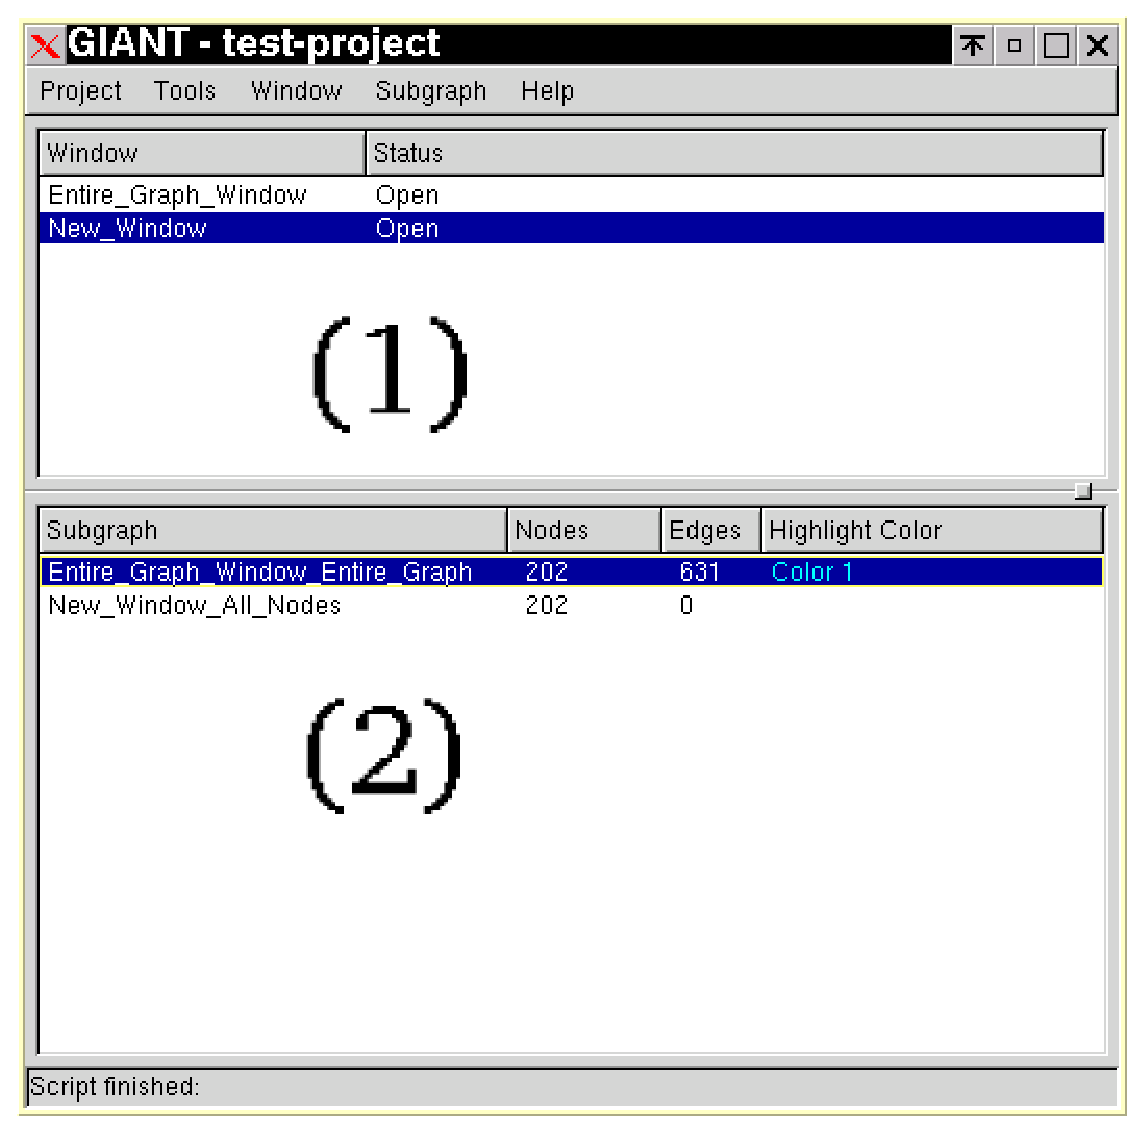
\includegraphics[scale=.75]{gui/main_window}
   \caption{Main-Window}
   \label{Main-Window-Pic}
\end{figure}

\clearpage

%Erg�nzungen by Martin
Jede Instanz von GIANT hat genau ein Hauptfenster. \index{Hauptfenster}
Im Hauptfenster (siehe Abbildung \ref{Main-Window-Pic}) werden die
Anzeigefenster und
IML-Teilgraphen des aktuell ge�ffneten Projektes (siehe  
\ref{Project Persistenz der Projekte}) in Listen angezeigt. 
�ber Popup-Men�s k�nnen IML-Teilgraphen
und Anzeigefenster manipuliert werden.

Im Fenster befinden sich zwei Listen, Window List (1) und
Subgraph List (2).


  \subsection {Titelzeile}
  In der Titelzeile wird \gq{GIANT - <Projektname>} dargestellt.
 
  \subsection {Men�leiste (Main Window)}
  In der Men�leiste befinden sich folgende Eintr�ge:

    \subsubsection {Untermen� Project} \label{Main-Window-Project}
      \begin{enumerate}
         \item {New}\\
         
         Hiermit wird ein neues Projekt angelegt. Ein eventuell bereits ge�ffnetes
         Projekt wird dabei geschlossen, wobei �nderungen auf Nachfrage 
         vorher gespeichert werden.

         \begin{itemize}
         
    \item{GIANT zeigt den Standard-Filechooser-Dialog und fordert den
    Benutzer auf, eine vorhandene IML-Graph Datei auszuw�hlen.}
    
    \item{GIANT zeigt erneut den Standard-Filechooser-Dialog und fordert den
    Benutzer zur Eingabe des Namens der Projektdatei auf. Die Dateiendung wird sp�ter
    von GIANT automatisch gesetzt.}
    
    \item {Der Name der Projektdatei ist
    automatisch auch der Name f�r das Projekt. Das Verzeichnis der
    Projektdatei wird automatisch zum Projektverzeichnis. Existiert die eingegebene Projektdatei bereits, 
    erscheint eine Fehlermeldung.
    Existiert in dem Projektverzeichnis bereits eine andere Projektdatei, so 
    erscheint ebenfalls eine Fehlermeldung.}
        \end{itemize}
    
         \item {Open}\\
         
         �ffnet ein GIANT Projekt. Ein eventuell bereits ge�ffnetes
         Projekt wird dabei geschlossen, wobei �nderungen auf Nachfrage 
         vorher gespeichert werden.
         \begin{itemize}
           \item {War vorher bereits ein Projekt offen, erscheint vorher eine
           Abfrage, ob dieses gespeichert werden soll.}
           \item {GIANT zeigt den Standard-Filechooser-Dialog und fordert
           den Benutzer zur Auswahl einer vorhandenen GIANT-Projektdatei auf.}
         \end{itemize}
         \item {Save}
         
         Speichert ein Projekt in die Verwaltungsdateien im Projektverzeichnis
         der neuen Projektdatei.
         
         \item {Save As...}
         
         Speichert ein Projekt in die Verwaltungsdateien im Projektverzeichnis
         der neuen Projektdatei unter neuem Namen.
         
         \begin{itemize}
          \item{Der Benutzer gibt im Standard-Filechooser-Dialog 
             das neue Projektverzeichnis 
             und den Namen f�r die neue Projektdatei ein, die Dateiendung 
             wird sp�ter von GIANT automatisch gesetzt.}
         \end{itemize}
         
         \item {Info}
         
         Zeigt einen Informationsdialog �ber den Graphen an.
         
         \item {Quit}
         
         Beendet das Programm GIANT.
         
      \end{enumerate}    
      
     \subsubsection {Untermen� Tools}  \label{Main-Window-Tools}
       \begin{enumerate}

          \item {GSL Editor...}
          
          Mit diesem Men�punkt kann ein GSL Script ausgef�hrt werden.
          Es erscheint der Skriptdialog, in den das Skript eingegeben
          werden kann. Es ist auch m�glich, Skripte zu laden oder zu
          speichern. Details hierzu finden sich unter \ref{GUI Anfragedialog}.
          
        \end{enumerate}
        
        
    \subsubsection {Untermen� Window}  
        \begin{enumerate}
          \item {New}\\
          Mit diesem Men�punkt kann ein neues leeres Fenster ge�ffnet werden.
        \end{enumerate}
    \subsubsection {Untermen� Subgraph}  
        \begin{enumerate}
          \item {New}\\
          Mit diesem Men�punkt kann ein neuer leerer IML-Teilgraph erstellt werden.
         \item {Set Operation}\\
          Mit diesem Men�punkt kann eine Mengenoperation auf IML-Teilgraphen
          durchgef�hrt werden, GIANT zeigt dazu den \gq{Set Operation Dialog},
          siehe Abschnitt \ref{Common-Set-Operation-Dialog}.
        \end{enumerate}
        

    \subsubsection {Untermen� Help}  \label{Main-Window-Info}     
       \begin{enumerate}
          \item {About..}\\
          Dieser Men�punkt gibt ein Fenster mit Informationen zur
          GIANT Programmversion und zu den Autoren aus.
        \end{enumerate}
     

  \subsection {Statuszeile}
  \label{Statuszeile}
  \index{Statuszeile}
  Die Statuszeile befindet sich ganz unten im Hauptfenster. In der
  Statuszeile werden Informationen zum aktuellen Zustand von GIANT
  dargestellt.

   \subsection {Window List (1)}
  
   Im Hauptfenster befindet sich zuoberst eine Liste \gq{Window List}, welche
   alle Anzeigefenster des Projektes (offen und geschlossen anzeigt).
   Eine Beschreibung, was alles mit einem Fenster gespeichert wird,
   befindet sich in Abschnitt \ref{Project Persistenz der Projekte}.
   
   \subsubsection {Inhalt Window List}
   \label{WINDOW-LIST}
   
   Window List hat die Spalten \gq{Window} und \gq{Status}. In
   \gq{Window} wird der Name aller Anzeigefenster dargestellt, in
   \gq{Status} befindet sich der Text "Open", wenn das Fenster
   ge�ffnet ist.
    
    \subsubsection {Popup-Men� Window List}
    
    
        Beim Rechtsklick auf Window List �ffnet sich ein 
        Popup-Men� mit folgenden Men�punkten:
        \label{WINDOW-LIST-POPUP}

        \begin{enumerate}
          \item Open\\
             �ffnet ein im Speicher vorhandenes, momentan geschlossenes Fenster.
          \item Close\\
             Schlie�t ein vorhandenes Fenster, es kann wieder ge�ffnet werden.
             Falls das Fenster noch nicht gespeichert wurde, wird eine
             Sicherheitsabfrage durchgef�hrt, ob gespeichert werden soll.
          \item Save Window\\
             Speichert ein Fenster im Projektverzeichnis.
          \item Rename Window\\
             �ndert den Namen eines Fensters, ein entsprechender Dialog erscheint.
          \item Delete Window\\
             L�scht ein Fenster aus dem Projektverzeichnis, es wird auch aus der Window List gel�scht.
        \end{enumerate}
    
  \subsection {Subgraph List (2)}
  \label{GUI Subgraph List}
    
    Unter der Window List befindet sich eine Liste \gq{Subgraph List} mit
    allen IML-Teilgraphen des Projektes.
   
    \subsubsection {Inhalt Subgraph List} 
    
      Subgraph List hat die folgenden Spalten:
      \begin{enumerate}
        \item Subgraph
        \item Nodes
        \item Edges
        \item Color
      \end{enumerate}
    
      In der Spalte Name stehen die Namen der existierenden IML-Teilgraphen,
      in Nodes die Anzahl der Graph-Knoten des jeweiligen IML-Teilgraphen, 
      in Edges die Anzahl der Graph-Kanten und in Highlighted befindet sich
      ein K�stchen in der
      Farbe, die f�r die Hervorhebung des IML-Teilgraphen verwendet wird.
      Bei nicht hervorgehobenen IML-Teilgraphen wird dieses K�stchen
      nicht angezeigt.

    
    \subsubsection {Popup-Men� Subgraph List}
    \label {Popup-Men� Subgraph List}
      Bei einem Rechtsklick auf Subgraph List �ffnet 
      sich ein Popup-Men� mit folgenden Men�punkten:
        \label{SUBGRAPH-LIST-POPUP}
        \begin{enumerate}
          \item Highlight (Men�)
            \begin{enumerate}
              \item Color 1
              \item Color 2
              \item Color 3\\
              Mit diesen drei Men�punkten kann der angew�hlte IML-Teilgraph
              in allen Fenstern in der ausgew�hlten Farbe markiert werden.
            \end{enumerate}
          \item Unhighlight In All Windows\\
             Mit diesen drei Men�punkten kann der angew�hlte IML-Teilgraph
              in allen Fenstern wieder entf�rbt werden, die Markierung also
              entfernt werden.
              
              
          \item Insert as Selection\\
             Mit diesem Men�punkt kann ein IML-Teilgraph als Selektion in ein
             Fenster kopiert werden. Nach Ausw�hlen dieser Funktion ist mit der
             Maus (linke Taste) in das Fenster zu klicken, in das der Subgraph
             eingef�gt werden soll, an eine passende Stelle zu klicken.
          \item Rename
             Mit dieser Funktion kann der Name eines IML-Teilgraphen ge�ndert werden,
             ein entsprechender Dialog erscheint nach der Auswahl dieses Punktes.
          \item Duplicate
             Mit dieser Funktion kann ein IML-Teilgraph dupliziert werden,
             ein Dialog zur Auswahl eines neuen Namens erscheint nach der
             Auswahl dieses Punktes.
          \item Delete
             Mit diesem Men�punkt kann ein IML-Teilgraph nach Sicherheitsabfrage
             gel�scht werden.
        \end{enumerate}   
        Als weitere Men�punkte im Popup-Men� erscheinen die im GIANT-Config-File
        definierten kontextsensitiven GSL-Skripte. Mehr Informationen hierzu finden
        sich in Abschnitt \ref{Config-GSL-Context-Scripts}.

\clearpage
\section {Anzeigefenster} \label{GUI Anzeigefenster}
\index{Anzeigefenster}

  \begin{figure}[!htbp]
     \centering
     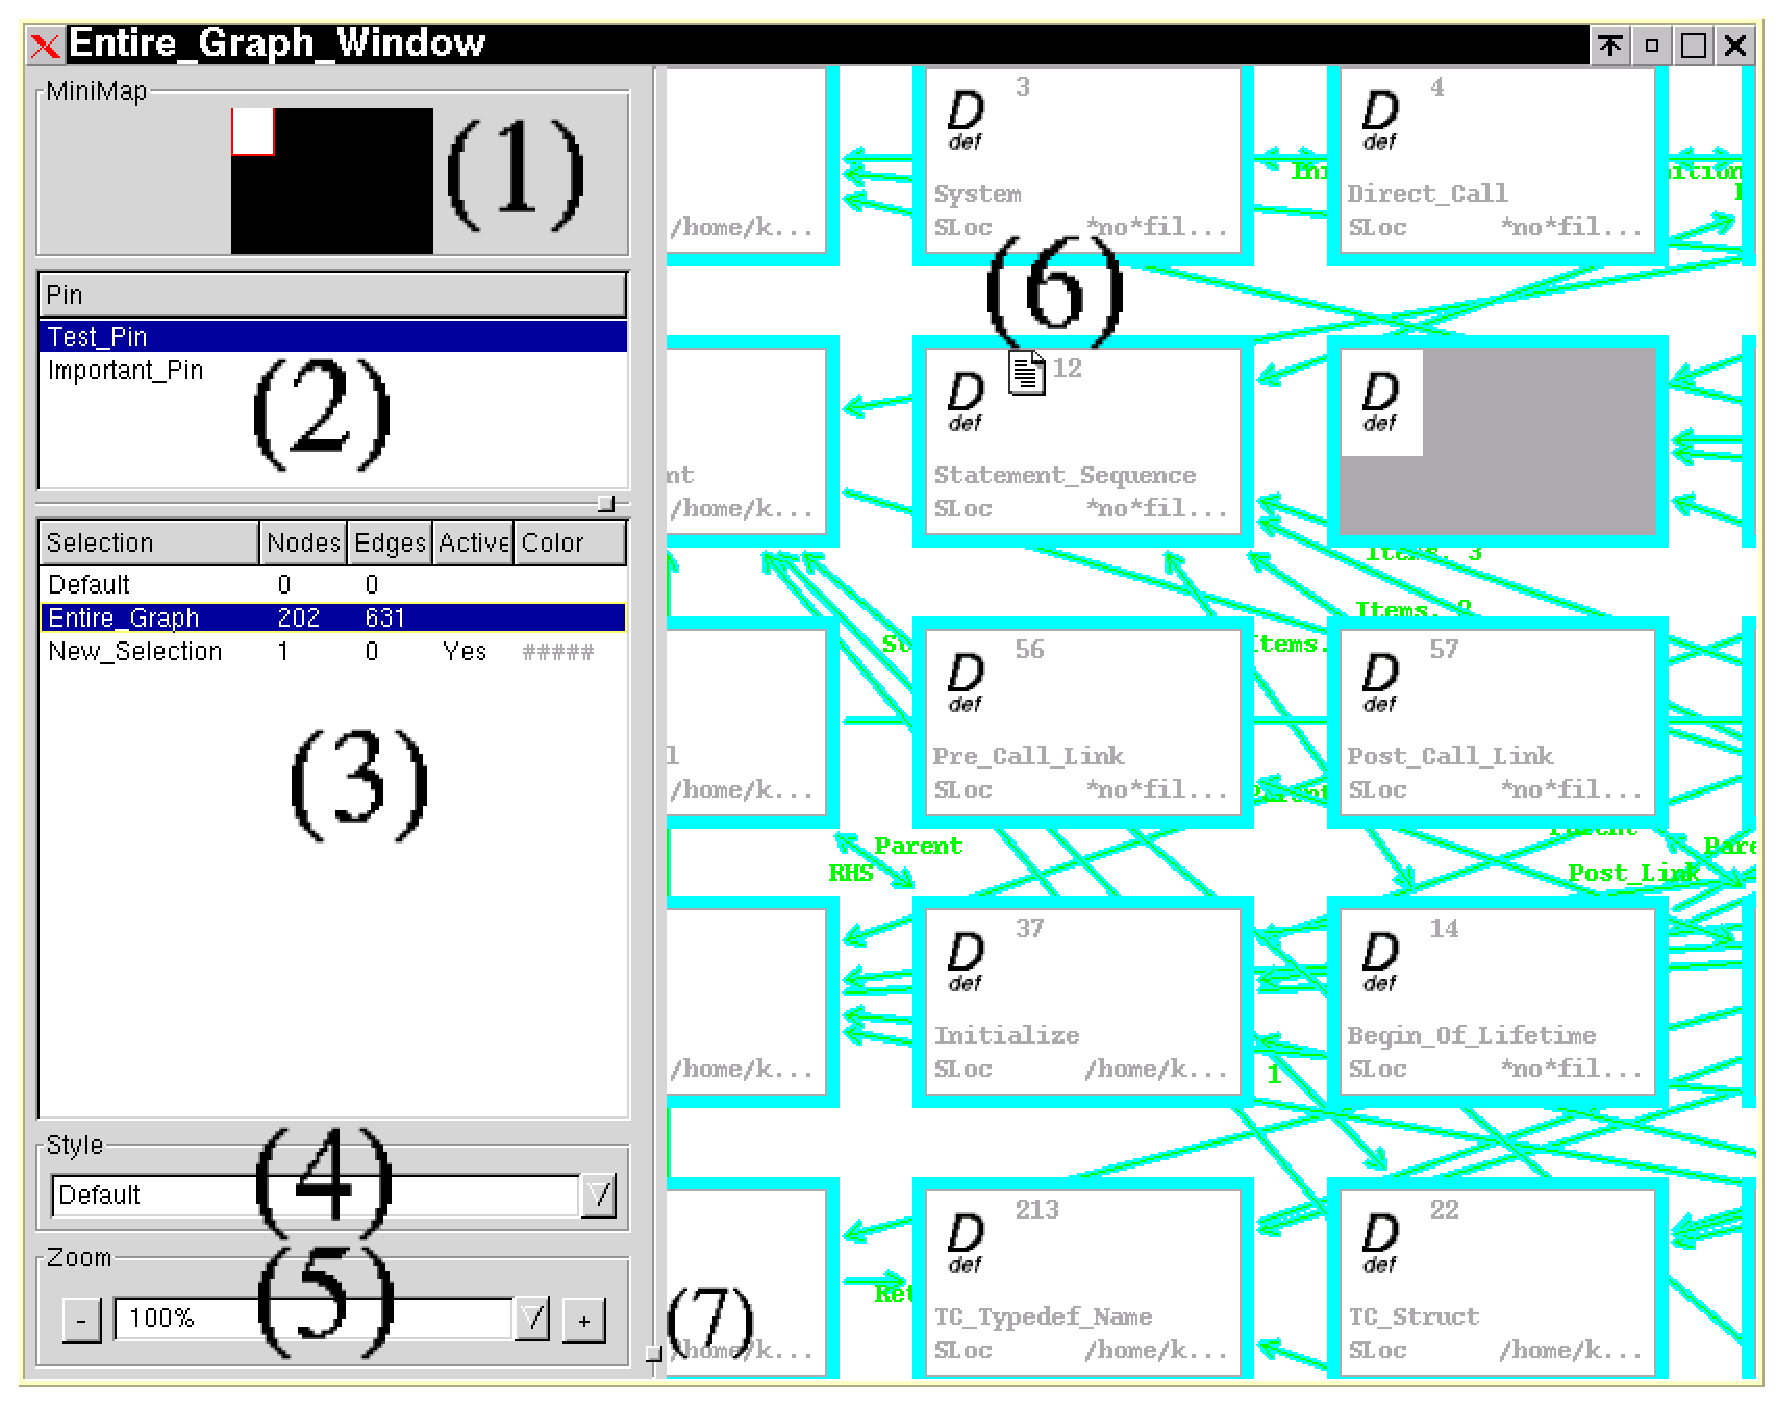
\includegraphics[width=16cm]{gui/visualization_window}
     \caption{Graph-Window}
     \label{Graph-Window-Pic}
  \end{figure}

  Im Programm kann es mehrere Anzeigefenster 
  (siehe Abbildung \ref{Graph-Window-Pic}) geben. 
  

  In Anzeigefenstern (Visualization Windows) werden Teile des IML-Graphen
  visualisiert.  Sie erscheinen im gro�en quadratischen rechten Teil
  (\gq{Vis Pane} (6)) des Fensters. Die Vis Pane enth�lt den Anzeigeinhalt
  des Fensters.  Im linken Teil des Fensters, der Toolbar
  (\gq{Vis Toolbar}) befinden sich untereinander die
  MiniMap (1), Pinliste (2), Selektionsliste (3), die Stilauswahl-Combobox (4) und die
  Zoom-Kontrolle (5). Dieser Teil kann durch Verschieben des entsprechenden
  Buttons (7) unten an der Trennleiste in der Gr��e ver�ndert werden.
  \index{Zoom-Kontrolle}
  \index{Visualisierungsstile!Stilauswahl-Combobox}

 \subsection {MiniMap (1)} \label{GUI Minimap}
 \index{Minimap} 
 
 In der MiniMap wird der Anzeigeinhalt verkleinert dargestellt,
 der Graph wird jedoch nur durch einen grauen Kasten repr�sentiert,
 Knoten sind nicht sichtbar. Die MiniMap wird von einem Rahmen
 umschlossen. Der sichtbare Anzeigeinhalt wird durch einen kleineren
 Rahmen repr�sentiert, der innerhalb der MiniMap durch Mausklicks
 versetzt werden kann. Je nach Zoomstufe ist dieser Rahmen gr��er
 oder kleiner. Wird der Rahmen versetzt, wird der sichtbare Anzeigeinhalt
 in der Vis Pane entsprechend angepasst.\\
 Vergr��ert sich die von Knoten bedeckte Fl�che im Fenster, z.B. durch
 Einf�gen von Teilgraphen, so ver�ndert sich auch die Minimap entsprechend.

  \subsection{Visualisierung der Knoten und Kanten (6)}

    In der Vis Pane werden die Fenster-Knoten und Fenster-Kanten angezeigt.
 
    \subsubsection{Node-Popup-Men�}\label{Node-Popup-Men�}
    
       Wenn auf einem Fenster-Knoten mit der rechten Maustaste geklickt wird, 
    �ffnet sich folgendes Popup-Men�:
    
    \begin{enumerate}
      \item Show Info\\
          Zeigt ein Fenster mit Informationen zum Knoten
      \item Show Source\\
          Zeigt den zum Knoten geh�renden Source Code in einem externen Editorfenster
      \item Annotate...
             Mit diesem Men�punkt l��t sich eine Annotation zu einem Knoten hinzuf�gen,
             �ndern oder l�schen.
             Der Knoten ist dann ggf. graphisch als annotiert gekennzeichnet.
             \label{Change Node Annotation}
             \label{Delete Node Annotation}
             \begin{itemize}
                \item{Der Nutzer f�hrt einen Rechtsklick auf den Knoten aus, den er
                       annotieren will und w�hlt im Popup-Men� \gq{Annotate...} an}
                \item{Im erscheinenden Knotenannotations-Dialog kann der Text der
                      Annotation eingegeben werden und mit OK best�tigt werden.
                      Mittels der Buttons Delete kann die Annotation gel�scht
                      werden, durch Cancel kann die bisherige Annotation beibehalten
                      werden.}
                \item{Nach dem n�chsten Speichern des Projektes ist die Annotation
                      dauerhaft erstellt.}
             \end{itemize}
        \end{enumerate}
        Als weitere Men�punkte im Popup-Men� erscheinen die im GIANT-Config-File
        definierten kontextsensitiven GSL-Skripte. Mehr Informationen hierzu finden
        sich in Abschnitt \ref{Config-GSL-Context-Scripts}.
              Mit diesem Men� k�nnen die GSL-Skripte im Untermen� schnell auf den
              Knoten bezogen ausgef�hrt werden, d.h. ihnen wird die ID des Knotens
              als Parameter �bergeben.
    
    \subsubsection{Background-Popup-Men�} \label{Background-Popup-Men�}
    Wenn in der Vis Pane mit der rechten Maustaste auf eine Stelle
    geklickt wird, an der kein Fenster-Knoten liegt, �ffnet sich das folgende
    Popup-Men�.

    \label{Empty Vis Pane Right click}
    \begin{enumerate}
      \item New Pin\\
         Mittels dieses Men�punktes kann ein neuer Pin (siehe \ref{VIS-PANE-Pins})angelegt werden.
         \begin{itemize} 
             \item{Der Benutzer f�hrt einen Rechtsklick auf den Anzeigeinhalt eines
                Anzeigefensters durch und w�hlt aus dem Popup-Men� 
                (siehe \ref{Empty Vis Pane Right click}) den Eintrag \gq{New Pin} aus.
                Der sp�ter erstellte Pin verweist dann auf die Stelle im Anzeigeinhalt,
                auf die der Rechtsklick durchgef�hrt wurde.}
             \item{Der Benutzer gibt im aufgehenden Texteingabedialog einen
                zul�ssigen Namen f�r den neuen Pin ein und best�tigt mit OK}
             \item{GIANT speichert die aktuelle Zoomstufe und die Position des sichtbaren
                Anzeigeinhaltes in einem neuen Pin.}
         \end{itemize}
      \item Make Room\\
        Mittels dieses Men�punktes k�nnen Knoten auseinandergeschoben werden,
        um Platz zu schaffen.
        \begin{itemize}
         \item{Der Nutzer f�hrt einen Rechtsklick auf eine leere Stelle des
         sichtbaren Anzeigeinhalts in einem Anzeigefenster durch und w�hlt im erscheinenden
         Popup-Men� \gq{Make Room} an}
         \item{GIANT zeigt in der Statuszeile im Hauptfenster 
               \gq{Select position in display window}.
                Der Benutzer gibt den Punkt um den herum die Fenster-Knoten (und damit
                automatisch auch die Fenster-Kanten) auseinander geschoben werden
                 sollen �ber den Fadenkreuzcursor vor.}
         \item{GIANT zeigt einen Dialog an, in dem der Benutzer ausw�hlt, um welchen 
               Betrag die Fenster-Knoten auseinander geschoben werden sollen.
               Der Benutzer w�hlt einen geeigneten Betrag aus und best�tigt mit OK. }    
         \item{GIANT schiebt die Knoten entsprechend auseinander.}
        \end{itemize}
        \item Select All\\
           Bei Auswahl dieses Men�punktes werden alle Knoten im Fenster selektiert.
        \item Select Nothing\\
           Bei Auswahl dieses Men�punktes wird bei allen Knoten im Fenster die
           Selektierung aufgehoben.
        Als weitere Men�punkte im Popup-Men� erscheinen die im GIANT-Config-File
        definierten kontextsensitiven GSL-Skripte. Mehr Informationen hierzu finden
        sich in Abschnitt \ref{Config-GSL-Context-Scripts}.
    \end{enumerate}
    
    \subsubsection{Kanten-Popup-Men�} \label{Kanten-Popup-Men�}
    Wenn in der Vis Pane mit der rechten Maustaste auf eine Kante
    geklickt wird, �ffnet sich ein Popup-Men�:
%*     \begin{itemize}
%*       \item Zoom to edge\\
%*         Dieser Men�punkt zoomt so, da� die gew�hlte Kante gut im Anzeigefenster
%*       sichtbar ist.
%*     \end{itemize}
        Als Men�punkte im Popup-Men� erscheinen die im GIANT-Config-File
        definierten kontextsensitiven GSL-Skripte. Mehr Informationen hierzu finden
        sich in Abschnitt \ref{Config-GSL-Context-Scripts}.
              Mit diesem Men� k�nnen die GSL-Skripte im Untermen� schnell auf die
              Kante bezogen ausgef�hrt werden, d.h. ihnen wird die ID der Kante
              als Parameter �bergeben.

  \subsection{Pins (2)} \label{VIS-PANE-Pins}
  \index{Pins}

    In der Pinliste (\gq{Pin List}) k�nnen Pins angesprungen oder ver�ndert werden.

    Im Popup-Men� der Pinliste befinden sich folgende Men�punkte:
    
    \begin{enumerate}
      \item Show\\
            Mittels dieses Men�punktes kann der sichtbare Anzeigeinhalt gem�� den im Pin gespeicherten
            Informationen gesetzt werden.
      \item Rename\\
            Mittels dieses Men�punktes kann der Name des Pins ge�ndert werden, ein
            entsprechender Dialog erscheint. 
      \item Delete\\
            Mittels dieses Men�punktes kann der Pin aus der Pinliste gel�scht werden.
    \end{enumerate}

  \subsection{Selektionsauswahlliste (3)} \label{Selektionsauswahlliste}
    Die Selektionsauswahlliste hat die Spalten \gq{Name} mit dem Namen der
    Selektion, \gq{Color} mit der Farbe der Selektion und \gq{Active}
    mit \gq{Yes} bei der aktiven Selektion.

    Im Popup-Men� der Selektionsauswahlliste (\gq{Selection List}) befinden
    sich folgende Eintr�ge:

    \begin{enumerate}
      \item Set Active\\
          Mittels dieser Funktion kann eine Selektion zur aktiven Selektion gemacht werden.
      \item Highlight (Men�)\\
        Diese Funktion dient zum Hervorheben von Selektionen innerhalb eines
        Anzeigefensters.
        War bereits eine andere Selektion mit der vom Benutzer gew�hlten
        Farbe hervorgehoben (die Farbe, welche im Popup-Men� der
        Selektionsauswahlliste unter \gq{Highlight Selection} gew�hlt wurde,
        so ist diese Selektion nicht mehr hervorgehoben.
        \begin{enumerate}
         \item Color 1\\
          Hebt in der im Config-File definierten Farbe 1 hervor
         \item Color 2\\
          Hebt in der im Config-File definierten Farbe 2 hervor
         \item Color 3\\
          Hebt in der im Config-File definierten Farbe 3 hervor
        \end{enumerate}
        Der Benutzer startet die Funktion mit einem Rechtsklick 
        auf die gew�nschte Selektion in der Selektionsauswahlliste
        und w�hlt im zugeh�rigen Popup-Men� das Untermen�
        \gq{Highlight Selection} und dort die gew�nschte Farbe aus.
        GIANT hebt die Selektion mit der ausgew�hlten Farbe hervor.
      \item Unhighlight Selection\\
        Diese Funktion dient dazu, die Hervorhebung von Selektionen innerhalb eines 
        Anzeigefensters aufzuheben.
        Der Benutzer startet die Funktion mit einem Rechtsklick 
        auf die gew�nschte Selektion in der
        Selektionsauswahlliste und w�hlt im zugeh�rigen Popup-Men� den Eintrag
        \gq{Unhighlight Selection} aus.
      \item Apply Layout\\
          Mittels dieser Funktion k�nnen Selektionen innerhalb
          eines Anzeigefensters layoutet werden.
          Die verf�gbaren Layoutalgorithmen sind in Kapitel 
          \gq{Layoutalgorithmen} beschrieben.
          \begin{itemize}
           \item{Der Benutzer w�hlt aus der Selektionsauswahlliste (siehe
            \ref{Selektionsauswahlliste}) die Selektion aus, deren
            Fenster-Knoten layoutet werden sollen. Hierzu f�hrt er einen
            Rechtsklick auf die Selektion durch und w�hlt im Popup-Men� den
            Eintrag \gq{Layout Selection} aus.}
           \item{GIANT zeigt einen Dialog zur Auswahl und Konfiguration des
            gew�nschten Layoutalgorithmus 
            (siehe \ref{Layoutalgorithmen-Dialog}). Der Benutzer w�hlt
            in diesem Dialog den gew�nschten Layoutalgorithmus aus.}
          \end{itemize}
      \item Set Operation\\
            Zus�tzlich zu den M�glichkeiten der Anfragesprache GSL (siehe Kapitel
            \ref{GIANT Scripting Language}) kann der Benutzer
            die g�ngigen Mengenoperationen, wie Mengenvereinigung, Schnitt und Differenz,
            auch direkt �ber einen entsprechenden Dialog 
            (siehe \ref{Common-Set-Operation-Dialog}) ausf�hren, welcher mit dieser
            Funktion aufgerufen werden kann.\\
      \item Insert As Subgraph\\
           Dieser Men�punkt leitet einen neuen IML-Teilgraphen aus einer
           Quell-Selektion ab.
           \begin{itemize}
             \item{Der Benutzer f�hrt einen Rechtsklick auf die Quell-Selektion in
                   der Selektionsauswahlliste aus
                   und w�hlt im Popup-Men� den Eintrag 
                   \gq{Create New IML Subgraph from This Selection} aus.}
             \item{GIANT zeigt den allgemeinen Texteingabedialog
                   an. Der Benutzer gibt einen Namen f�r den neu zu erstellenden IML-Teilgraphen
                   ein und best�tigt mit OK.
                   Gibt der Benutzer hier keinen Namen ein, so vergibt GIANT automatisch 
                   einen Namen.}
           \end{itemize}
      \item Rename\\
           Mit dieser Funktion kann der Name einer Selektion ge�ndert werden, GIANT zeigt
           einen entsprechenden Dialog.
      \item Duplicate\\
           Mit dieser Funktion kann eine Selektion dupliziert werden, GIANT fragt in einem
           entsprechenden Dialog nach dem Namen der neuen Selektion.
      \item Zoom To Selection
         Der im Fenster sichtbare Anzeigeinhalts wird durch automatisches Zoomen
         und Scrollen so ver�ndert, dass die ausgew�hlte Selektion vollst�ndig
         sichtbar ist.
      \item Delete\\
           Diese Funktion dient zum L�schen von Selektionen innerhalb eines 
           Anzeigefensters. Hierdurch bleiben die Fenster-Knoten und Fenster-Kanten
           unver�ndert. Die Standard-Selektion (siehe \ref{Standard-Selektion}) kann
           nicht gel�scht werden. Wurde die aktuelle Selektion gel�scht (siehe 
           \ref{Aktuelle Selektion vs Selektionen}), so wird die
           Standard-Selektion zur aktuellen Selektion. Die Fenster-Knoten und
           Fenster-Kanten,  die zur gel�schten Selektion geh�ren, werden nicht
           gel�scht. War die Selektion hervorgehoben, so wird die
           Hervorhebung der Fenster-Knoten und Fenster-Kanten aufgehoben.
           \begin{itemize}
            \item{Der Benutzer startet die Funktion durch Rechtsklick auf die zu
              l�schende Selektion in der Selektionsauswahlliste (siehe 
              \ref{Selektionsauswahlliste}) und w�hlt aus dem Popup-Men� den Eintrag
              \gq{Delete Selection} aus. Falls der Benutzer die Standard-Selektion 
              (siehe \ref{Standard-Selektion}) ausgew�hlt hat, ist der Eintrag
              \gq{Delete Selection} deaktiviert.}
             \item{GIANT l�scht die entsprechende Selektion.}
           \end{itemize}
      \item Delete With Content\\
           Mittels dieser Funktion k�nnen alle Fenster-Knoten und Fenster-Kanten
           einer Selektion aus einem Anzeigefenster gel�scht werden
           (siehe auch \ref{Verhalten beim Entfernen von Fenster-Knoten und 
           Fenster-Kanten}).\\
           Falls die gew�hlte Selektion nicht die Standard-Selektion war,
           ist die Selektion jetzt aus dem Anzeigefenster gel�scht und taucht nicht
           mehr in der Liste �ber die Selektionen auf.
           Wurde die Standard-Selektion (siehe \ref{Standard-Selektion}) 
           gew�hlt, so wird diese nicht aus dem Anzeigefenster gel�scht, sondern
           ist jetzt leer.
           \begin{itemize}
             \item{Der Benutzer f�hrt einen Rechtsklick auf die entsprechende Selektion in der
                   Selektionsauswahlliste durch (siehe \ref{Selektionsauswahlliste})
                   und w�hlt im Popup-Men� den Eintrag \gq{Delete Nodes and Edges
                   of Selection} aus.}
             \item{GIANT zeigt die Sicherheitsabfrage (siehe \ref{Sicherheitsabfrage}) 
                   und fragt nach, ob es die Selektion samt ihrer Fenster-Knoten und 
                   Fenster-Kanten wirklich l�schen soll (\gq{Really delete Selection 
                   from its window including Nodes and Edges?}).
                   Der Benutzer best�tigt mit Yes.}
             \item{GIANT l�scht die Selektion samt allen zugeh�rigen Fenster-Knoten und
                   Fenster-Kanten aus dem entsprechenden Anzeigefenster.
                   Wurde die Funktion f�r die Standard-Selektion
                   (siehe \ref{Standard-Selektion}) ausgef�hrt, so werden die
                   Fenster-Knoten und Fenster-Kanten aus dem Anzeigeinhalt gel�scht, 
                   die Standard-Selektion selbst wird geleert aber nicht gel�scht.} 
           \end{itemize}

            
    \end{enumerate}    


  \subsection{Stilauswahl-Combobox (4)}
  \label{GUI Stilauswahl-Combobox}   

    In der Stilauswahl-Combobox (\gq{Style Chooser}) kann ein 
    Visualisierungsstil (siehe auch \ref{Config Visualisierungsstile})
    ausgew�hlt werden.

  \subsection{Zoom-Kontrolle (5)} \label{GUI Zoom-Kontrolle}  

    Die Zoom-Kontrolle besteht aus folgenden Elementen:
    
  \begin{enumerate}
      \item Button \gq{-} % OK
      \item Combobox mit vorgefertigten Zoom-Werten und Eingabem�glichkeit und Button \gq{OK}.
      \item Button \gq{+} % OK
  \end{enumerate}    

%  In der ComboBox zur Zoom-Kontrolle befindet sich
%  neben den vorgegebenen Zoomstufen \index{Zoomstufe} noch der
%  Eintrag \gq{Whole Graph}, welcher daf�r sorgt, da� der gesamte Graph im
%  Fenster sichtbar ist.
%  Nach Auswahl einer Zoomstufe in der Combobox mu� der Button \gq{OK}
%  geklickt werden.
  
  Mittels der Buttons \gq{+}und \gq{-} kann die Zoomstufe nach oben bzw. unten
  ver�ndert werden, pro Klick ver�ndert sie sich um einen bestimmten Betrag.
 
    \subsection{Scrollen}
    \label{Scrolleisten}
    
    Der sichtbare Anzeigeinhalt kann folgendermassen gescrollt werden:
    \begin{itemize}
      \item{Durch Bewegen des sichtbaren Bereiches in der Minimap mit der Maus}
      \item{Durch Klicken mit der linken Maustaste auf eine leere Stelle des 
            sichtbaren Anzeigeinhalts, festhalten der Maustaste und Bewegen des
            Mauszeigers aus dem Fenster heraus in die entsprechende Richtung
            (oben, unten, links oder rechts).}
    \end{itemize}

\clearpage
\section{Knoten-Informationsfenster} \label{Knoten-Informationsfenster}

    \begin{figure}[!htbp]
       \centering
       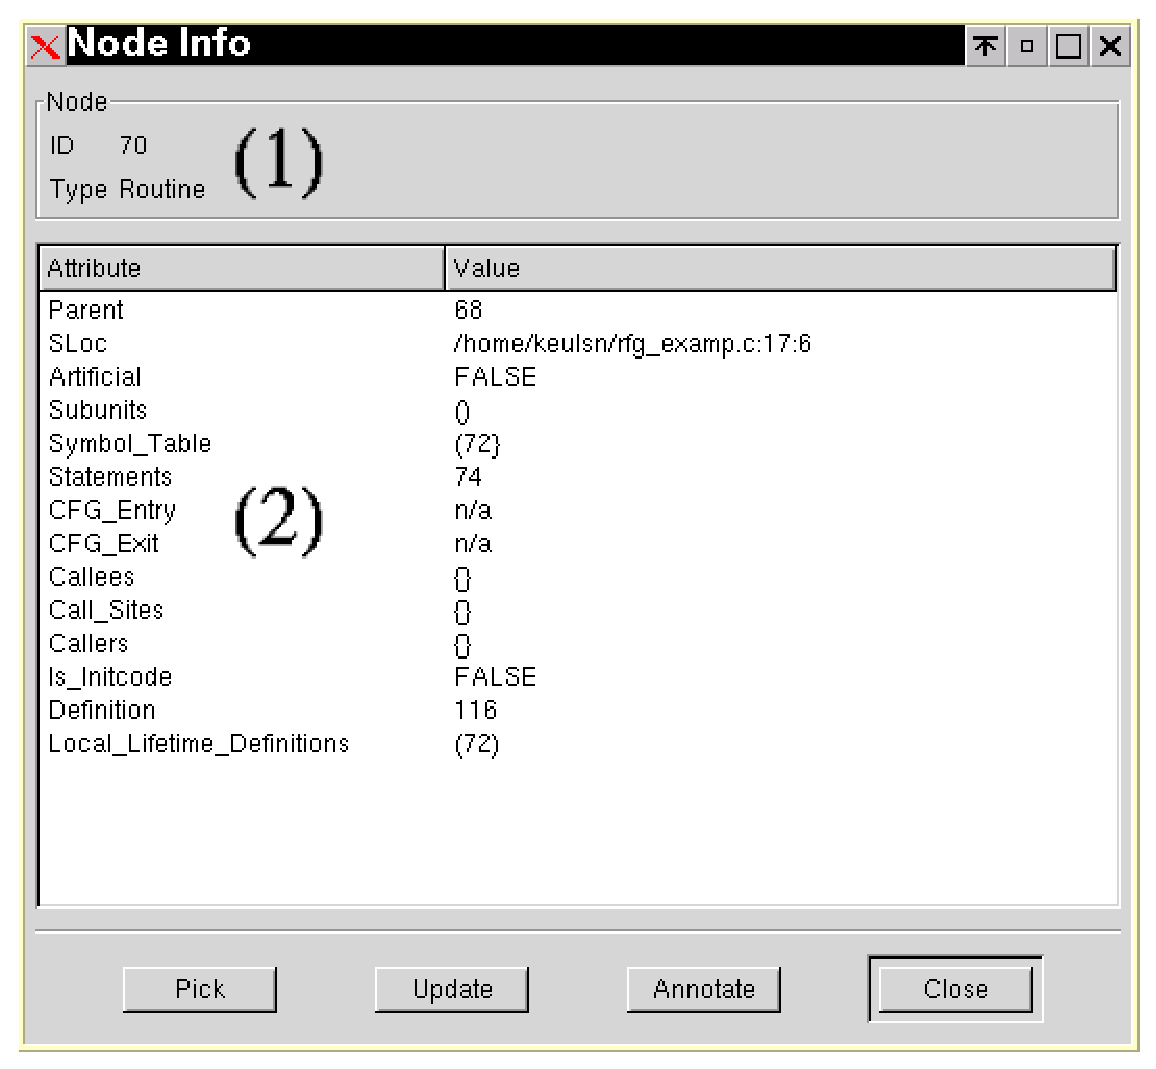
\includegraphics[scale=0.6]{gui/node_information_dialog}
       \caption{Node-Info-Window}
       \label{Node-Info-Window-Pic}
    \end{figure}

    In Knoten-Informationsfenstern (siehe Abbildung 
    \ref{Node-Info-Window-Pic}) 
    k�nnen n�here Informationen zu Fenster-Knoten angezeigt werden.\\
    
    Im Knoten-Informationsfenster wird die ID und die Knotenklasse des 
    vom Fenster-Knoten repr�sentierten IML-Knotens dargestellt (1),
    darunter befindet sich die Liste \gq{Attributes} mit den Attributen
    des Knotens (2).\\
    
    Unter der Liste (2) befinden sich nebeneinander die Buttons
    \gq{Pick}, \gq{Update}, \gq{Annotate} und \gq{Close}. 
    \gq{Pick} dient zur Auswahl eines anderen Fenster-Knotens 
    mittels des Fadenkreuzcursors, dazu wird nach Klicken von \gq{Pick}
    ein Fensterknoten angeklickt.\\
    
    \gq{Update} dient zur Aktualisierung der Liste, Annotate �ffnet das
    Knoten-Annotationsfenster (siehe Abschnitt \ref{Knoten Annotations-Dialog}).\\
    
    Die Informationen zu dem ausgew�hlten
    Fenster-Knoten werden dann im Knoten-Informationsfenster dargestellt.\\
    
    Das Knoten-Informationsfenster enth�lt, neben der Anzeige von Knoten-ID
    und Knoten-Typ, die Liste \gq{Attributes}:

    Die Liste Attributes enth�lt die Attribute des Knotens und hat
    zwei Spalten:
    
      \begin{enumerate}
        \item Name  (der Name des Attributes)
        \item Value (der Attributwert)
      \end{enumerate}
    

\clearpage
\section{Skriptdialog} \label{GUI Anfragedialog}

    \begin{figure}[!htbp]
       \centering
       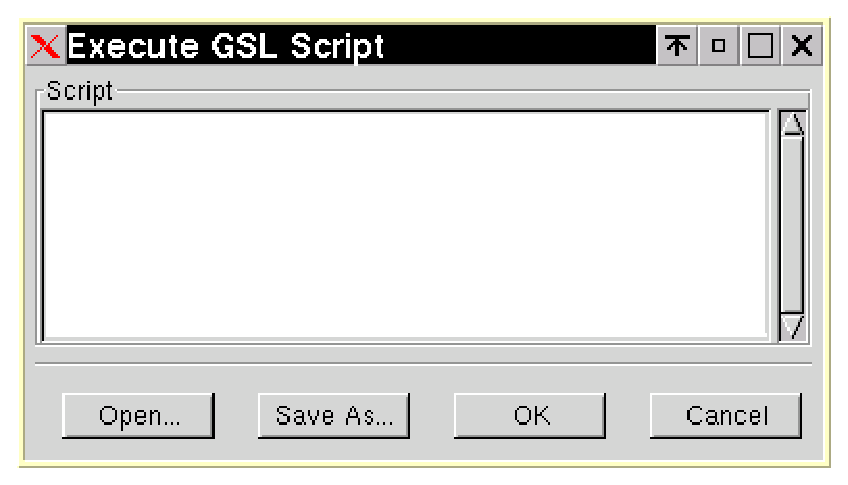
\includegraphics[scale=0.75]{gui/query_dialog}
       \caption{Skript-Dialog}
       \label{Skript-Dialog-Pic} 
    \end{figure}

Der Skriptdialog (siehe Abbildung \ref{Skript-Dialog-Pic})
hat zuoberst ein Textfeld,
in das ein GSL Skript eingegeben werden kann.

Unter Query Text befinden sich folgende Buttons:

      \begin{enumerate}
        \item Open...\\
           Mit diesem Button kann ein auf Festplatte gespeichertes Skript geladen werden.
           Nach Klick auf diesen Button erscheint ein Dateiauswahlfenster, nach Auswahl
           eines Skriptes wird dieses in das Textfeld eingef�gt.
        \item Save As...\\
           Mit diesem Button kann das im Textfeld eingetippte Skript gespeichert werden.
           Nach dem Klick auf diesen Button erscheint ein Dateiauswahlfenster, nach
           Festlegen eines Dateinamens wird das Skript unter diesem Namen gespeichert.
        \item Okay\\
           F�hrt das eingegebene Skript aus.
        \item Cancel
           Schlie�t das Fenster ohne Ausf�hrung oder Speicherung des Skriptes.
      \end{enumerate}
      
\clearpage
\section{Allgemeiner Texteingabedialog}
\label{DIALOG-WINDOW}

    \begin{figure}[!htbp]
       \centering
       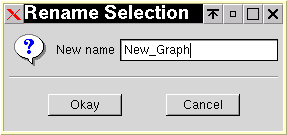
\includegraphics{gui/input_dialog}
       \caption{Dialog-Window}
       \label{Dialog-Window-Pic}
    \end{figure}

Ein allgemeiner Texteingabedialog ist ein Fenster Dialog Window 
(siehe Abbildung \ref{Dialog-Window-Pic}) mit dem
Titel \gq{Input}. Im Fenster ist ein einzeiliges Textfeld
mit einem Prompt-Text, zwei Buttons mit den Beschriftungen \gq{OK}
und \gq{Cancel}.

%\clearpage
\section{Set-Operation-Dialog}
\label{Common-Set-Operation-Dialog}

    \begin{figure}[!htbp]
       \centering
       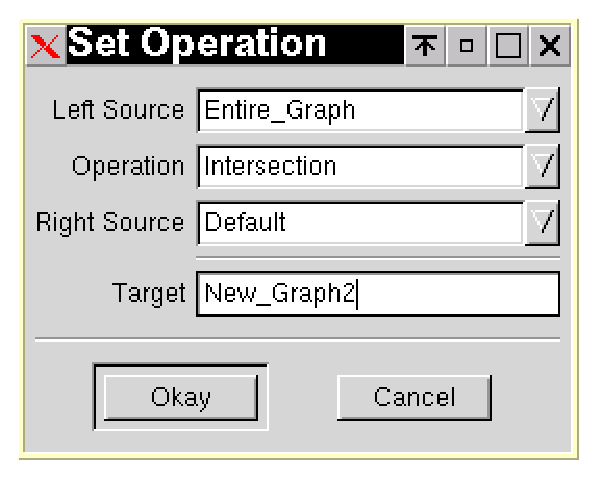
\includegraphics[scale=0.85]{gui/set_operation_dialog}
       \caption{Set-Operation-Dialog}
       \label{Set-Operation-Dialog-Pic}
    \end{figure}


Der Set-Operation-Dialog (siehe Abbildung \ref{Set-Operation-Dialog-Pic}) 
dient dazu, Mengenoperationen �ber 
Selektionen und
IML-Teilgraphen durchzuf�hren.
Die Mengenoperation l�sst sich wie folgt beschreiben:\\
TARGET := LEFT\_SOURCE <Operation> RIGHT\_SOURCE \\


Bestandteile des Dialoges sind:
\begin {enumerate}

 \item Left Source Combobox\\
 Soll eine Mengenoperation f�r Selektionen ausgef�hrt werden, so kann hier eine der
 Selektionen des entsprechenden Anzeigefensters ausgew�hlt werden.\\
 Bei einer Mengenoperation �ber IML-Teilgraphen, werden alle IML-Teilgraphen
 des Projektes angezeigt, von denen dann einer ausgew�hlt werden kann.
 
 \item Operation Combobox\\
 Mengenoperation, die ausgef�hrt werden soll; ausw�hlbar sind: Union, Difference oder Intersection.

 \item Right Source Combobox\\
 Soll eine Mengenoperation f�r Selektionen ausgef�hrt werden, so kann hier eine der
 Selektionen des entsprechenden Anzeigefensters ausgew�hlt werden.\\
 Bei einer Mengenoperation �ber IML-Teilgraphen, werden alle IML-Teilgraphen
 des Projektes angezeigt, von denen dann einer ausgew�hlt werden kann..
 
 \item Target Textfeld\\
 Name der neuen Selektion oder des neuen IML-Teilgraphen als Ergebnis
 der Mengenoperation.
 
 \item Buttons OK und Cancel\\
 Mit den beiden Buttons OK und Cancel l�sst sich die Operation starten bzw.
 der Dialog ohne Ausf�hren der Operation verlassen.
 
\end {enumerate}

 \clearpage
\section {Layoutalgorithmen Dialog}\label{Layoutalgorithmen-Dialog}

    \begin{figure}[!htbp]
       \centering
       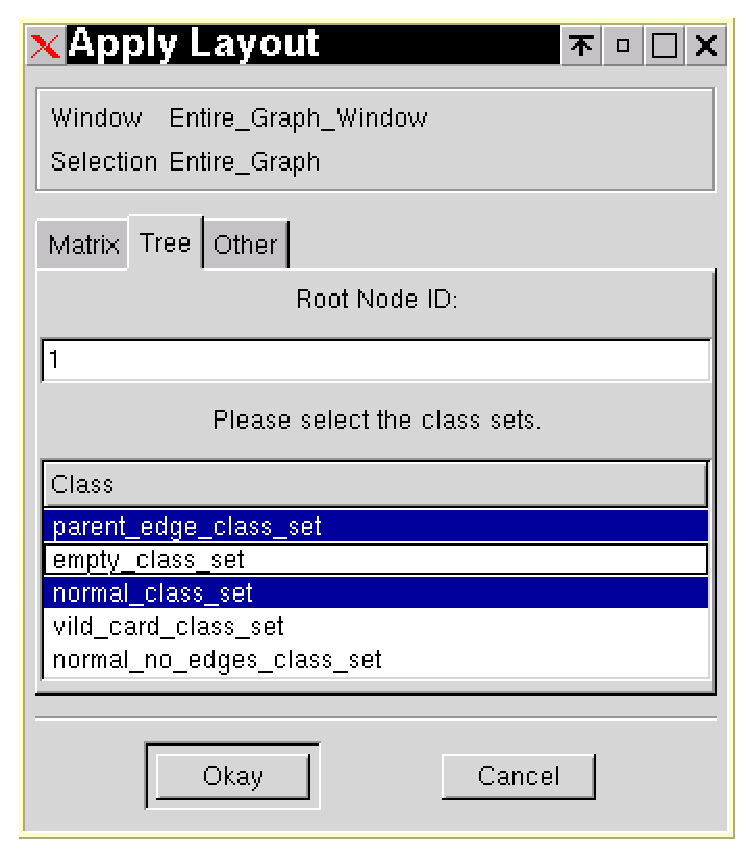
\includegraphics{gui/apply_layout_dialog}
       \caption{Layout-Algorithmen-Dialog}
       \label{Layout-Algorithm-Dialog-Pic}
    \end{figure}

Der Layoutalgorithmen Dialog (siehe Abbildung \ref{Layout-Algorithm-Dialog-Pic}) 
wird �ber Popup-Men�s auf Selektionen aufgerufen und bietet folgende M�glichkeiten:

\begin {enumerate} 
 \item Anzeige der zu layoutenden Selektion mit dem zu layoutenden Fenster (1)
 \item {Auswahl des Layoutalgorithmus}\\
       �ber die Tabs (4) im Fenster kann der Layoutalgorithmus ausgew�hlt werden,
       in der aktuellen Version stehen zur Auswahl: Matrix, Tree Layout,
       Other (f�r sp�tere Erweiterungen).\\
       Das Tree-Layout ordnet die Knoten als Baum an, dessen Wurzel anhand
       der ID des Knotens (welche u.a. mit dem Knoten-Informationsfenster, siehe
        \ref{Knoten-Informationsfenster}, festgestellt
       werden kann) festgelegt wird.\\
       Das Matrix-Layout ordnet die Knoten in einer Matrix an.\\
       
 \item Ggf.\ Eingabefeld f�r die ID des Wurzelknotens bei Treelayouts (2)
 \item {Ggf.\ Auswahl der f�r das Layout der Knoten zu ber�cksichtigenden Klassenmengen (3)
        (class sets, siehe \ref{Config-Klassenmengen} und \ref{Klassenmenge}) bei semantischen Tree-Layouts.}\\
        Nur Klassenmengen, die in der Liste per Mausklick markiert worden sind
        (Mehrfachmarkierungen sind m�glich), werden f�r das Layout
        ber�cksichtigt. Falls keine Klassenmengen angeben wurden,
        werden alle Kanten, {\em auch diejenigen, die nicht im Fenster
        sichtbar sind,} f�r das Layout verwendet.
 \item OK Button
 \item Cancel Button
\end {enumerate}

Nach dem Klicken von OK ist mit der linken Maustaste in ein Fenster auf den
dargestellten Anzeigeinhalt zu klicken (an einer leere Stelle), an dieser
Position wird dann die neu layoutete Selektion eingef�gt.

\clearpage
\section{Dateneingabe}
Beschreibung von verschiedenen GUI Elementen zur Eingabe von Daten.

\subsection{Knoten-Annotations-Dialog}
\label{Knoten Annotations-Dialog}

    \begin{figure}[!htbp]
       \centering
       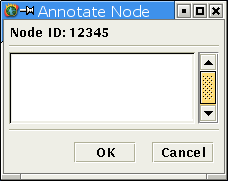
\includegraphics{gui/annotate_node}
       \caption{Node-Annotation-Dialog}
       \label{Node-Annotation-Dialog-Pic}
    \end{figure}
  
Der Knoten-Annotations-Dialog (siehe Abbildung 
\ref{Node-Annotation-Dialog-Pic}) besteht aus einem Fenster mit einem
Label, welches die ID des Knotens anzeigt, und einem Textfeld f�r den Annotationstext.
Mittels der beiden Buttons Okay und Cancel k�nnen die �nderungen im
Textfeld �bernommen oder verworfen werden. Der Button Delete kann dazu
verwendet werden, das Textfeld zu leeren.
\index{Knoten-Annotationen}


%  \clearpage
\subsection{Platz Schaffen-Dialog}
\label{Platz Schaffen-Dialog}

    \begin{figure}[!htbp]
       \centering
       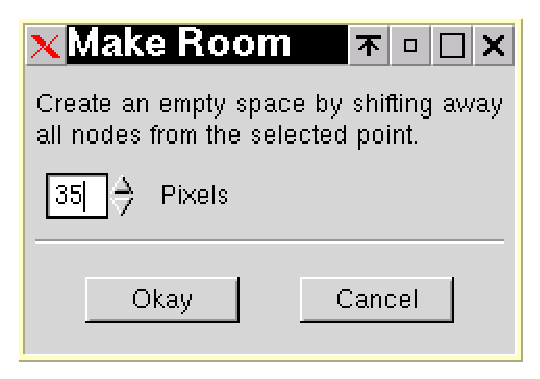
\includegraphics{gui/make_room}
       \caption{Make-Room-Dialog}
       \label{Make-Room-Dialog-Pic}
    \end{figure}

Im Dialogfenster Make Room (siehe Abbildung \ref{Make-Room-Dialog-Pic}) 
wird in einem Textfeld als Zahl 
eingegeben, um wie viel
Pixel die Fenster-Knoten an einer vorher markierten Stelle auseinandergeschoben 
werden sollen.
Mit dem Button Okay kann best�tigt werden, mit dem Button Cancel abgebrochen werden.

\clearpage
\section{Ausgabe von Fehlermeldungen}
\label {GUI Ausgabe von Fehlermeldungen}

    \begin{figure}[!htbp]
       \centering
       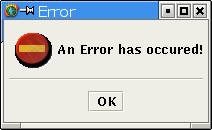
\includegraphics{gui/error_dialog}
       \caption{Error-Window}
       \label{Error-Window-Pic}
    \end{figure}

Im Fenster eines allgemeinen Fehlerdialoges (siehe Abbildung \ref{Error-Window-Pic})
befindet sich die Fehlermeldung und ein \gq{OK}-Button, mit dem das
Fenster geschlossen werden kann.. 

\section{Sicherheitsabfrage}\label{Sicherheitsabfrage}
\index{Sicherheitsabfrage}

    \begin{figure}[!htbp]
       \centering
       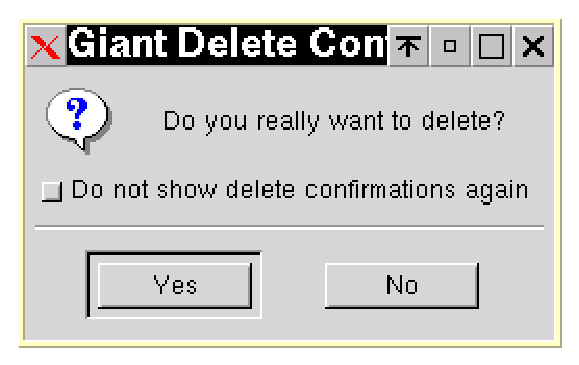
\includegraphics{gui/confirmation_dialog}
       \caption{Confirmation-Window}
       \label{Confirmation-Window-Pic}
    \end{figure}
    
Eine allgemeine Sicherheitsabfrage (siehe Abbildung \ref{Confirmation-Window-Pic}) 
besitzt einen
Fragetext und die zwei Buttons \gq{Yes} und \gq{No}.
Ggf. kann mit einem Radiobutton festgelegt werden, da� Sicherheitsabfragen
des jeweiligen Types in Zukunft nicht mehr angezeigt werden (z.B. \gq{Do not
show delete confirmations again}).

\clearpage

\section{Auswahl von Dateien}

  \subsection {Der \gq{Standard-Filechooser-Dialog}}
  \label {Standard-Filechooser-Dialog}

    \begin{figure}[!htbp]
       \centering
       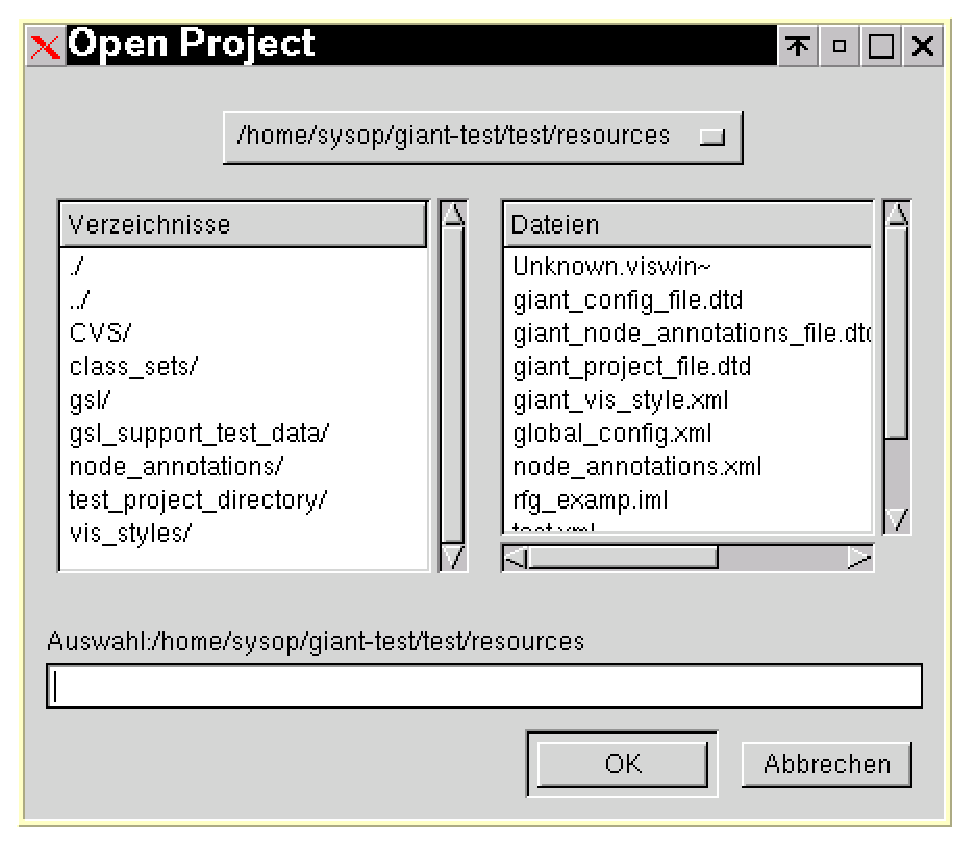
\includegraphics{gui/filechooser_dialog}
       \caption{Filechooser-Window}
       \label{Filechooser-Window-Pic}
    \end{figure}

Die Auswahl von Dateien (Laden/Speichern) passiert bei GIANT mittels
des Standard-Filechooser-Dialogs (siehe Abbildung \ref{Filechooser-Window-Pic}). 
Dieser Dialog ist Bestandteil der Widget-Bibliothek von GTK.


% ******** Gibt es den Fadenkreuz-Cursor?
\section{Fadenkreuz-Cursor}
\label{Fadenkreuzcursor}
        Der Cursor verwandelt sich nach Auswahl bestimmter
        Funktionen (siehe z.B. Funktion \ref{Platz Schaffen-Dialog}) in ein Fadenkreuz.
        Durch Linksklick auf einen Fenster-Knoten oder eine 
        Fenster-Kante in einem Anzeigefenster  
        wird diese(r) f�r die jeweilige Funktion ausgew�hlt. 
        Der Fadenkreuz-Cursor wird auch zur Vorgabe von Positionen,
        an denen dann z.B. neue Fenster-Knoten eingef�gt werden,
        verwendet.
        Nach dem Linksklick  verwandelt
        sich der Fadenkreuz-Cursor wieder in den Standard-Cursor.
        Durch einen Rechtsklick bei aktivem Fadenkreuz-Cursor l�sst sich 
        die aktuelle Funktion abbrechen.




%%% Local Variables: 
%%% TeX-master: "spec"
%%% End: 



%===============================================================================
% 
% Anfragesprache
%
\chapter{GIANT Scripting Language}
\label {GIANT Scripting Language}

Die F�higkeiten der GIANT Scripting Language (GSL) werden im Anhang 
\gq{GSL}, der Teil der GIANT Spezifikation ist, beschrieben.


%===============================================================================
% 
% Projektverwaltung
%
\chapter{GIANT Projektverwaltung}
\label{GIANT Projektverwaltung}

In diesem Kapitel wird beschrieben, wie persistente Arbeitsergebnisse
von GIANT strukturiert und gespeichert werden.
Arbeitsergebnisse sind z.B. vom Benutzer erzeugte Anzeigefenster
mit als Fenster-Knoten visualisierten IML-Knoten eines IML-Graphen.
Soweit f�r das Verst�ndnis von GIANT n�tig, sind auch Interna des
Programms festgehalten.

% ==============================================================================
%  $RCSfile: project.tex,v $, $Revision: 1.17 $
%  $Date: 2003/02/25 14:33:49 $
%  $Author: squig $
%
%  Description:
%
% ==============================================================================


%===================
\section {Persistenz �ber Projekte}

GIANT speichert persistente Informationen in so genannten Projekten.
\begin {enumerate}

  \item 
  Wird w�hrend des Betriebs von GIANT ein neues Projekt angelegt, so erh�lt 
  es automatisch eine Projektdatei.
  
  \item
  Ein Projekt besteht aus einem Verweis auf eine IML-Graph-Datei, auf die sich
  die gespeicherten Informationen beziehen, sowie aus den gespeicherten 
  Informationen f�r IML-Teilgraphen, Anzeigefenster und Knoten-Annotationen.
 
  \item
  Jedes Projekt hat einen vom Benutzer definierbaren Namen, dieser Name 
  entspricht dem Namen der Projektdatei und wird innerhalb des IML-Browsers 
  angezeigt.

  \item
  Der Name eines bereits angelegten Projektes kann mit den Mitteln von 
  GIANT nicht ge�ndert werden (au�er dadurch, dass  man das Projekt unter 
  neuem Namen neu speichert). 

  \item
  Der Benutzer kann beliebig viele Projekte anlegen.
  
  \item
  In GIANT darf immer nur ein Projekt gleichzeitig ge�ffnet sein. 
  
  \item
  W�hrend der Arbeit mit GIANT kann jederzeit ein Projekt geladen oder ein
  neues Projekt angelegt werden. 
  Voraussetzung hierf�r ist allerdings, dass dies 
  in der Reflektion zum IML-Graphen unterst�tzt wird.
  
  \item
  GIANT wei� nicht, ob ein geladenes Projekt gegen�ber den f�r das Projekt
  in der Projektdatei und in den Verwaltungssdateien gespeicherten 
  Informationen modifiziert wurde oder nicht.

\end {enumerate}


  \subsection {Das Projektverzeichnis}
  \begin {enumerate}

    \item  
    S�mtliche Dateien, die die Informationen f�r ein Projekt enthalten,
    befinden sich in diesem Verzeichnis. 

    \item
    In einem Projektverzeichnis darf nur ein Projekt abgelegt werden.
    
  \end {enumerate}    


  \subsection {Die Projektdatei}
  \begin {enumerate}

    \item
    Die Projektdatei liegt als XML-Datei vor.

    \item
    Die Projektdatei befindet sich im Projektverzeichnis und enth�lt 
    Informationen, die zur Identifikation des zu einem Projekt geh�renden 
    IML-Graphen n�tig sind. 
  
    \item
    Der Name der Projektdatei entspricht dem Namen des Projektes.

    \item
    Die Projektdatei enth�lt Referenzen zu allen Dateien, die Bestandteil
    des Projektes sind (Verwaltungsdateien f�r IML-Teilgraphen und
    Anzeigefenster und die Verwaltungsdatei f�r Knoten-Annotationen).

    \item
    Der Pfad zu der Datei, die den IML-Graphen enth�lt, ist in der Projektdatei 
    gespeichert. 
  \end {enumerate}
  
 
  \subsection {Pr�fung der IML-Graph Datei}
  Die Reflektion muss f�r jede IML-Graph Datei eine m�glichst eindeutige 
  Pr�fsumme berechnen k�nnen. Beim Laden eines Projektes wird �berpr�ft, 
  ob die in der Projektdatei gespeicherte Pr�fsumme
  der Pr�fsumme der zu ladenden IML-Graph Datei entspricht. 
  Das Verhalten von GIANT f�r den Fall, dass eine IML-Graph Datei geladen wird, 
  die zwar die passende Pr�fsumme hat, aber nicht den IML-Graphen enth�lt, 
  der dem Projekt eigentlich zu Grunde liegt, ist undefiniert.


  \subsection {Verwaltungsdateien f�r Anzeigefenster}
 
  \begin {enumerate}
  
    \item
    Zu jedem Anzeigefenster gibt es eine Verwaltungsdatei. 
    
    \item
    Diese Verwaltungsdatei enth�lt alle Informationen zur kompletten 
    Rekonstruktion eines Anzeigefensters. Alle Informationen werden
    in bin�rer Form gespeichert.
 
  \end {enumerate}
  Insbesondere werden folgende Informationen gespeichert:
 
  \begin {enumerate}
 
    \item Der komplette Anzeigeinhalt 
          (alle visualisierten Knoten und Kanten mit Position).
    \item Alle Pins (gespeicherte sichtbare Anzeigeinhalte).
    \item Alle dem Anzeigefenster bekannten Selektionen.
 
  \end {enumerate}
 
  Der f�r das Anzeigefenster gew�hlte Visualisierungsstiel wird zwar mit 
  gespeichert, da die Viualisierungsstiele v�llig unabh�ngig von den 
  Projekten �ber Konfigurationsdateien realisiert werden, 
  kann nicht gerantiert werden, dass der gew�nschte Stiel beim Laden 
  des Projektes auch wieder gefunden wird,
  in diesem Fall wird dann ein \gq{Standard-Stil} verwendet.


  \subsection {Verwaltungsdateien f�r IML-Teilgraphen}
  \begin {enumerate}

   \item
    F�r jeden IML-Teilgraphen gibt es eine eigene Verwaltungsdatei.
    
    \item
    S�mtliche erzeugten IML-Teilgraphen werden in Verwaltungsdateien in 
    bin�rer Form gespeichert. 

  \end{enumerate}
  
  
  \subsection {Die Verwaltungsdatei f�r Knoten-Annotationen}
  \begin {enumerate}

   \item
   Alle Knoten-Annotationen werden in einer Verwaltungsdatei gespeichert.
   
   \item
   Diese Datei liegt als XML Datei vor.
  \end{enumerate}
  

 
 
%===================
\section {Grundlegendes Verhalten von GIANT beim Speichern von Projekten} 
  

  \subsection{\gq{Alles Speichern}}\label{Alles Speichern}
  Diese Funktionalit�t wird von entsprechenden UseCases genutzt. 
  Hierbei werden alle Anzeigefenster, IML-Teilgraphen 
  und Knoten-Annotationen in die Verwaltungsdateien geschrieben, 
  wobei alle �nderungen an noch offenen Anzeigefenstern ber�cksichtigt 
  werden.\\
 

  %===
  \subsection {Persistenz von Anzeigefenstern}
  \begin {enumerate}

    \item
    S�mtliche dem Projekt bekannten Anzeigefenster (alle Anzeigefenster zu 
    denen es eine entsprechende Verwaltungsdatei gibt) werden auf der GUI in 
    der Liste �ber die Anzeigefenster angezeigt, egal ob sie ge�ffnet sind
    oder nicht. 

    \item 
    Zu jedem Anzeigefenster eines Projektes gibt es eine Verwaltungsdatei,
    beim �ffnen eines neuen Fensters wird diese Datei automatisch mit
    erzeugt.

    \item
    Wird ein ge�ffnetes Anzeigefenster geschlossen, 
    so fragt GIANT nach, ob es eventuelle �nderungen speichern soll
    oder nicht. Falls ja, werden eventuelle �nderungen in die f�r das 
    Anzeigefenster vorhandene Verwaltungsdatei geschrieben, 
    anderenfalls bleibt der Zustand des Anzeigefensters nach der letzten
    Speicherung vorhanden (die zugeh�rige Verwaltungsdatei wird nicht 
    ver�ndert).

    \item
    Modifikationen (z.B. das Verschieben von Knoten) 
    auf einem Anzeigefenster werden nicht automatisch
    nach deren Durchf�hrung gespeichert (so kann notfalls ein
    Undo durchgef�hrt werden).

    \item
    Ein zu einem Projekt geh�rendes Anzeigefenster kann gel�scht werden, 
    hierbei werden alle Information �ber das Anzeigefenster einschlie�lich
    der Verwaltungsdatei vernichtet.
    >>>>>>>>>>>>>>>>USE CASE - L�schen persistenter Anzeigefenster
  \end {enumerate}

  %===
  \subsection {Persistenz von IML-Teilgraphen}
  \begin {enumerate}

    \item
    Alle in einem Projekt bereits vorhandenen IML-Teilgraphen werden auf der 
    GUI angezeigt (in einer entsprechenden Liste).
  
    \item
    Neu erzeugte IML-Teilgraphen und �nderungen an bestehenden 
    IML-Teilgraphen k�nnen �ber \gq{alles Speichern} (siehe oben) 
    gespeichert werden.
       
    \item
    Wird das Programm beendet, ohne das zuvor \gq{Alles Speichern} ausgef�hrt 
    worden ist, so gehen  alle nicht gespeicherten Informationen zu den 
    IML-Teilgraphen verloren (alle zwischenzeitlich ausgef�hrten Modifikationen 
    und alle zwischenzeitlich neu erzeugten IML-Teilgraphen). 
    Der Zustand des Projektes  nach dem letzten Speichern bleibt dann erhalten.

    \item
    Modifikationen an bestehenden IML-Teilgraphen werden nicht automatisch 
    gespeichert, zu neu erzeugten IML-Teilgraphen wird nicht automatisch
    eine Verwaltungsdatei erzeugt.
    \\
    N�TIG; DA SONST ANFRAGEN EVENTUELL AUSGEBREMST.
    IM GEGENSATZ ZU ANZEIGEFENSTERN KANN MAN IML-TEILGRAPHEN NICHT �FFNEN
    IM GEGENSATZ ZU ANZEIGEFENSTERN (fliegen beim Schlie�en aus dem
    speicher raus) WERDEN ALL IML-TEILGRAPHEN pauschal im
    SPEICHER GEHALTEN.

    \item
    IML-Teilgraphen k�nnen gel�scht werden. Falls vorhanden, wird dann auch
    die entsprechende Verwaltungsdatei ebenfalls sofort gel�scht.
  \end {enumerate}
  
  
  
\subsection {Persistenz von Knoten-Annotationen}
  \begin {enumerate}
  
   \item
   �nderungen bestehender oder neu erzeugte Knoten-Annotationen werden nur
   �ber die Funktionali�t unter \gq{alles Speichern} in die 
   Verwaltungsdatei geschrieben.
   
   \item
   Einmal erzeugte Knoten-Annotationen werden jedem IML-Knoten mit der 
   entsprechenden ID zugeordnet, egal in welchem Anzeigefenster diese
   visualisiert sind. Ein Knoten kann auch annotiert sein, wenn er in keinem
   Anzeigefenster visualisiert ist. Wird ein annotierter Knoten gel�scht 
   (aus einem Anzeigefenster entfernt), so wird der dazu vorhandene 
   Eintrag f�r die Annotation in der Verwaltungsdatei nicht automatisch mit gel�scht.
   
   >>>>>>>>>>>>>>>> EVENTUELL M�SSEN WIR HIER EINEN FILTER BAUEN
   DER KNOTEN-Annotationen entfernt, die nicht mehr gebraucht werden.
   
 \end {enumerate}
  
  
  
  
  
  
  
  
  


%===============================================================================
% 
% Beschreibung aller Konfigurationsdateien
%
\chapter{Konfiguration von GIANT}
\label{Konfiguration von GIANT}

Hier wird beschrieben, wie benutzerdefinierbare Einstellungen von
GIANT gespeichert und verwaltet werden. In diesem Kapitel wird 
insbesondere beschrieben, welche Einstellungen der Benutzer
in welchen Konfigurationsdateien vornehmen kann.

% ==============================================================================
%  $RCSfile: config.tex,v $, $Revision: 1.35 $
%  $Date: 2003/04/21 01:13:30 $
%  $Author: schwiemn $
%
%  Description:
%
%  Last-Ispelled-Revision: 1.19
%
% ==============================================================================


\section {Allgemeines} \index{Konfiguration}
\begin {enumerate}

  \item
  S�mtliche konfigurierbaren Einstellungen werden in XML-Dateien vorgenommen.
  F�r die verschiedenen Dateitypen werden auch
  Dokumenttyp-Definitionen (DTDs) erstellt.
  
  \item \label{config-allgemeines-punkt2}
  \index{Konfigurationsdatei!globale}
  Es gibt genau eine \gq{globale Konfigurationsdatei}. Zudem kann es beliebig 
  viele weitere XML-Dateien zur Konfiguration der weiter unten beschriebenen 
  Visualisierungsstile geben.\\
  Diese Dateien liegen in einem von GIANT fest vorgegebenen Verzeichnis.
  
  \item \index{Konfigurationsdatei!benutzerdefinierte}
  Die unter Punkt \ref{config-allgemeines-punkt2} beschriebenen Dateien zu
  Konfiguration k�nnen vom Benutzer auch in einem separaten 
  Unterverzeichnis seines Home-Verzeichnisses abgelegt werden. Findet
  GIANT beim Start ein derartiges Verzeichnis, so werden die
  Einstellungen aus der dort vorgefundenen Konfigurationsdatei, sowie
  die dort vorgefundenen Visualisierungsstile geladen.
 
\end {enumerate}


\section {Die globale Konfigurationsdatei} \index{Konfigurationsdatei}
Diese Datei ist in XML verfasst. In Ihr k�nnen die anschlie�end beschriebenen
Einstellungen vorgenommen werden.

%EVENTUELL F�R JEDEN BENUTZER EIGENE KONFIGURATIONS-DATEI VORSEHEN.

  \subsection {Verweise auf GSL-Skripte} 
  \index{Makros}
  \index{GSL!Makros}
  Es k�nnen GSL-Skript-Makros definiert werden. Jeder Makro wird durch 
  einen eindeutigen Namen und durch einen Verweis
  auf die Datei, welche das GSL-Skript enth�lt, spezifiziert.
  Der Makro kann dann aus einem Popup-Men� heraus aufgerufen werden, wobei
  dann das in der Datei stehende GSL Skript ausgef�hrt wird.

  \subsection {Farbe von Hervorhebungen}
  \index{hervorheben!Farben konfigurieren}
  Einstellung der Farben, mittels derer Selektionen oder IML-Teilgraphen 
  hervorgehoben werden.
  \begin {enumerate}
    \item Eine beliebige Farbe f�r die aktuelle Selektion.
    \item Beliebige Farben f�r das
          Hervorheben weiterer Selektionen.
    \item Beliebige Farben f�r das 
          Hervorheben von IML-Teilgraphen.
  \end {enumerate}

  \subsection {Editor zur Anzeige des Quellcodes}
  \label{Konfig Editor zur Anzeige des Quellcodes}
  \index{Editoren!Anzeige des Quellcodes}

  Der Benutzer legt in der globalen Konfigurationsdatei fest, 
  mit welchem Editor der zu IML-Knoten korrespondierende
  Quellcode automatisch angezeigt wird (unterst�tzt werden Emacs und vi). 

\section {Visualisierungsstile} \label{Config Visualisierungsstile}
\index{Visualisierungsstile!Konfiguration}
\index{Konfiguration!Visualisierungsstile}

Der Benutzer kann beliebig viele Visualisierungsstile definieren.
Mittels dieser Visualisierungsstile kann die Darstellung von
Fenster-Knoten und Fenster-Kanten dynamisch zur Laufzeit ge�ndert werden
(siehe auch 
\ref{Den Visualisierungsstil eines Anzeigefensters �ndern}).
Weitere Informationen zur Visualisierung von Fenster-Knoten und
Fenster-Kanten sind unter den Abschnitten
\ref{Visualization Visualisierung von Kanten} und
\ref{Visualization Visualisierung von Knoten} zu finden.\\
F�r die Visualisierungsstile gelten die folgenden Konventionen:


\begin {enumerate}

  \item
  F�r jeden Visualisierungsstil muss es eine entsprechende XML-Datei geben. 

  \item
  Ein Visualisierungsstil beschreibt, wie die Knoten und Kanten des 
  IML-Graphen innerhalb eines Anzeigefensters graphisch dargestellt 
  werden k�nnen.

  \item
  In einem Visualisierungsstil k�nnen klassenspezifische Einstellungen 
  vorgenommen werden, die nur f�r Knoten und Kanten gelten, 
  die zu der entsprechenden Klasse geh�ren.
  Bei jeder klassenspezifischen Einstellung f�r Knoten und Kanten kann daher 
  eine Liste der betroffenen Knoten- und Kantenklassen angegeben werden, 
  f�r die diese Einstellungen gelten sollen.

  \item
  Wird eine Kanten- oder eine Knotenklasse innerhalb eines
  Visualisierungsstils mehreren klassenspezifischen Einstellungen zugeordnet,   
  f�hrt dies zu keinem Fehler, es bleibt aber unspezifiziert, 
  welche Einstellung tats�chlich genommen wird.

  \item
  Es gibt jeweils eine Standard-Einstellung, die f�r alle
  Knoten- und Kantenklassen genommen wird, f�r die keine
  extra klassenspezifischen Einstellungen vorgenommen wurden.

  \item \index{Visualisierungsstile!Standard-Visualisierungsstil}
  Es gibt immer einen von GIANT fest
  vorgegeben Standard-Visualisierungsstil. Dieser Visualisierungsstil
  wird f�r neu erzeugte Anzeigefenster genommen. 
  Kann GIANT den einem Anzeigefenster zugewiesenen Visualisierungsstil
  nicht finden (falls die zugeh�rige XML-Datei fehlt) wird ebenfalls
  der Standard-Visualisierungsstil genommen. 

\end {enumerate}


  \subsection {Name des Visualisierungsstils}
  Jeder Visualisierungsstil erh�lt einen Namen. Unter diesem Namen ist der 
  Visualisierungsstil f�r jedes Anzeigefenster einzeln ausw�hlbar.
 
  \subsection {Einstellungen innerhalb des Visualisierungsstils}
    \begin{enumerate}
      \item Die Hintergrundfarbe im Anzeigefenster.

     % \item Wann Kanten im sichtbaren Anzeigeinhalt angezeigt werden sollen.
 
     %  \subitem Nur falls Start- und Zielknoten ebenfalls im sichtbaren 
     %           Anzeigeinhalt.
     %  \subitem Auch anzeigen falls nur Startknoten im sichtbaren 
     %           Anzeigeinhalt.
     %  \subitem Auch anzeigen falls nur Zielknoten im sichtbaren Anzeigeinhalt.
     %  \subitem Auch anzeigen falls weder Start- und Zielknoten im sichtbaren 
     %           Anzeigeinhalt. 
    \end{enumerate}


  \subsection {Klassenspezifische Einstellungen f�r Knoten}
  \index{Visualisierungsstile!klassenspezifische Einstellungen}

  Folgende  Einstellungen k�nnen f�r Knotenklassen vorgenommen werden. 
  Es muss eine Standard-Einstellung erstellt werden, die f�r alle
  Knotenklassen angewendet wird, f�r die nichts anderes definiert ist.
  \begin{enumerate}  
  

    \item Ein Icon f�r die Knotenklasse (Verweis auf eine entsprechende 
          Bilddatei). Das Icon muss im Pixmap-Format 
          vorliegen. Die Gr��e des Icons ist beliebig, bei zu gro�en
          Icons wird abgeschnitten. Es wird garantiert, dass Icons
          bis zu einer Gr�\ss e von 32*32 Pixel komplett dargestellt werden
          k�nnen.

    \item Eine Liste der Attribute der Knotenklasse, welche direkt innerhalb 
          des Anzeigefensters in dem \gq{Rechteck} f�r den Knoten dargestellt 
          werden sollen.
    \item Die Farbe der Schrift, mit der die Informationen innerhalb
          des Knoten-Rechtecks dargestellt werden.
    \item Die F�llfarbe des \gq{Rechtecks} in welchem die Attribute zu dem 
          Knoten dargestellt werden.
    \item Die Rahmenfarbe des \gq{Rechtecks}.
    
  \end{enumerate}

  
  \subsection {Klassenspezifische Einstellungen f�r Kanten}
  Folgende Einstellungen k�nnen f�r Kantenklassen vorgenommen werden.
  Es muss eine Standard-Einstellung erstellt werden, die f�r alle
  Kantenklassen angewendet wird, f�r die nichts anderes definiert ist.
  \begin{enumerate}
    \item Die Farbe der Kante.
    \item Die Farbe der Kantenbeschriftung.
    \item Die Art der Linie der Kante (normal, gestrichelt).
    \item Ob die Kante mit ihrer Kantenklasse beschriftet werden soll oder 
          nicht.
  \end{enumerate}

  Eine Kantenklasse wird durch die Knotenklasse des Start-Knotens 
  und durch den Namen des Attributes, welches die Kante darstellt, 
  eindeutig festgelegt (siehe Begriffslexikon). 
  Will der Benutzer nun Einstellungen f�r
  Kantenklassen vornehmen, kann er sich entweder auf genau eine
  Kantenklasse \gq{Start-Knotenklasse.Attributname} beziehen oder
  mittels eines Platzhalters auch auf mehrere:

  \begin{enumerate}
    \item Der Benutzer kann mittels des Platzhalters \gq{*}
          eine klassenspezifische Einstellung f�r
          alle Kanten, deren Start-Knoten zu einer bestimmten
          Knotenklasse geh�rt, 
          vornehmen -- also \gq{Start-Knotenklasse.*}.

   \item  Der Benutzer kann mittels des Platzhalters \gq{*}
          eine klassenspezifische Einstellung f�r
          alle Kanten, bei denen das sie repr�sentierende Attribut
          den gleichen Namen hat,
          vornehmen -- also \gq{*.Attributname}.
 
  \end{enumerate}

  
\section {Skript-Dateien} 
\label {Config Anfrage-Dateien}
\index{GSL!Skriptdateien} \index{Skriptdateien}

Eine Skript-Datei ist eine Textdatei, die genau ein GSL Skript enth�lt.
Auf diese Art und Weise k�nnen komplexe Skripte gespeichert und 
wiederverwendet werden.\\
Geladen werden k�nnen solche Dateien beim Kommandozeilenaufruf 
(siehe \ref{fa Starten von GIANT})
oder im Dialog zur Eingabe eine Skripts 
(vgl.\ UseCase \ref{UC Anfrage laden}).
F�r eine exakte Spezifikation der GSL siehe Kapitel 
\ref {GIANT Scripting Language}. 



%==============================================================================
%
%  Index
%
\printindex

%==============================================================================
% 
% Anhang
%
\newpage
\appendix

\end{document}
